% Festlegung des Allgemeinen Dokumentenformats
\documentclass[a4paper,12pt,headsepline]{scrartcl}

%%%%%%%%%%%%%%%%%%%%%
\usepackage{algorithm}
\usepackage{algorithmic}
%%%%%%%%%%%%%%%%%%%%%

\usepackage[numbers]{natbib}

% Umlaute unter UTF8 nutzen
\usepackage[utf8]{inputenc}

% Variablen
%Variablen welche innerhalb der gesamten Arbeit zur Verfügung stehen sollen
\newcommand{\titleDocument}{Deep Reinforcement Learning}
\newcommand{\subjectDocument}{Wie wirkt sich die visuelle Augmentation des Environments \\ auf die Generalisierung eines RL-Agenten in Procgen aus?}
%%Variablen welche innerhalb der gesamten Arbeit zur Verfügung stehen sollen
\newcommand{\titleDocument}{Deep Reinforcement Learning}
\newcommand{\subjectDocument}{Wie wirkt sich die visuelle Augmentation des Environments \\ auf die Generalisierung eines RL-Agenten in Procgen aus?}



% weitere Pakete
% Grafiken aus PNG Dateien einbinden
\usepackage{graphicx}

% Deutsche Sonderzeichen und Silbentrennung nutzen
\usepackage[ngerman]{babel}

% Eurozeichen einbinden
\usepackage[right]{eurosym}

% Zeichenencoding
\usepackage[T1]{fontenc}

\usepackage{lmodern}

% floatende Bilder ermöglichen
%\usepackage{floatflt}

% mehrseitige Tabellen ermöglichen
\usepackage{longtable}

% Unterstützung für Schriftarten
%\newcommand{\changefont}[3]{ 
%\fontfamily{#1} \fontseries{#2} \fontshape{#3} \selectfont}

% Packet für Seitenrandabständex und Einstellung für Seitenränder
\usepackage{geometry}
\geometry{left=3.5cm, right=2cm, top=2.5cm, bottom=2cm}

% Paket für Boxen im Text
\usepackage{fancybox}

% bricht lange URLs "schön" um
\usepackage[hyphens,obeyspaces,spaces]{url}

% Paket für Textfarben
\usepackage{color}

% Mathematische Symbole importieren
\usepackage{amssymb}

% auf jeder Seite eine Überschrift (alt, zentriert)
%\pagestyle{headings}

% erzeugt Inhaltsverzeichnis mit Querverweisen zu den Abschnitten (PDF Version)
\usepackage[bookmarksnumbered,pdftitle={\titleDocument},hyperfootnotes=false]{hyperref}
%\hypersetup{colorlinks, citecolor=red, linkcolor=blue, urlcolor=black}
%\hypersetup{colorlinks, citecolor=black, linkcolor= black, urlcolor=black}

% neue Kopfzeilen mit fancypaket
\usepackage{fancyhdr} %Paket laden
\pagestyle{fancy} %eigener Seitenstil
\fancyhf{} %alle Kopf- und Fußzeilenfelder bereinigen
\fancyhead[L]{\nouppercase{\leftmark}} %Kopfzeile links
\fancyhead[C]{} %zentrierte Kopfzeile
\fancyhead[R]{\thepage} %Kopfzeile rechts
\renewcommand{\headrulewidth}{0.4pt} %obere Trennlinie
%\fancyfoot[C]{\thepage} %Seitennummer
%\renewcommand{\footrulewidth}{0.4pt} %untere Trennlinie

% für Tabellen
\usepackage{array}

% Runde Klammern für Zitate
%\usepackage[numbers,round]{natbib}

% Festlegung Art der Zitierung - Havardmethode: Abkuerzung Autor + Jahr
\bibliographystyle{alphadin}

% Schaltet den zusätzlichen Zwischenraum ab, den LaTeX normalerweise nach einem Satzzeichen einfügt.
%\frenchspacing

% Paket für Zeilenabstand
\usepackage{setspace}

% für Bildbezeichner
\usepackage{capt-of}

% für Stichwortverzeichnis
\usepackage{makeidx}

% für Listings
\usepackage{listings}
\lstset{numbers=left, numberstyle=\tiny, numbersep=5pt, keywordstyle=\color{black}\bfseries, stringstyle=\ttfamily,showstringspaces=false,basicstyle=\footnotesize,captionpos=b}
\lstset{language=java}


%%%%%%%%%%%%%%%%%%
\usepackage[font=small,labelfont=bf]{caption}



%TEST
%\usepackage{titlesec}

%\titleclass{\subsubsubsection}{straight}[\subsection]


%\titleformat{\subsubsubsection}
%  {\normalfont\normalsize\bfseries}{\thesubsubsubsection}{1em}{}
%\titlespacing*{\subsubsubsection}
%{0pt}{3.25ex plus 1ex minus .2ex}{1.5ex plus .2ex}

%\def\toclevel@subsubsubsection{4}
%\def\toclevel@paragraph{5}
%\def\toclevel@paragraph{6}
%\def\l@subsubsubsection{\@dottedtocline{4}{7em}{4em}}
%\def\l@paragraph{\@dottedtocline{5}{10em}{5em}}
%\def\l@subparagraph{\@dottedtocline{6}{14em}{6em}}
%\makeatother

%\setcounter{secnumdepth}{4}
%\setcounter{tocdepth}{4}
%%%%%%%%%%%%%%%%%%


% Indexerstellung
\makeindex

\pagestyle{empty}

% Abkürzungsverzeichnis
\usepackage[german]{nomencl}
\let\abbrev\nomenclature

% Abkürzungsverzeichnis LiveTex Version
% Titel des Abkürzungsverzeichnisses
\renewcommand{\nomname}{Abkürzungsverzeichnis}
% Abstand zwischen Abkürzung und Erläuterung
\setlength{\nomlabelwidth}{.25\textwidth}
% Zwischenraum zwischen Abkürzung und Erläuterung mit Punkten
\renewcommand{\nomlabel}[1]{#1 \dotfill}
% Variation des Abstandes der einzelnen Abkürzungen zu einander
\setlength{\nomitemsep}{-\parsep}
% Index mit Abkürzungen erzeugen
\makenomenclature
%\makeglossary

% Abkürzungsverzeichnis TeTEX Version
% \usepackage[german]{nomencl}
% \makenomenclature
% %\makeglossary
% \renewcommand{\nomname}{Abkürzungsverzeichnis}
% \AtBeginDocument{\setlength{\nomlabelwidth}{.25\columnwidth}}
% \renewcommand{\nomlabel}[1]{#1 \dotfill}
% \setlength{\nomitemsep}{-\parsep}

% Optional: Einzelne Zeilen am Anfang einer Seite unterdrücken (Schusterjungen)
% \clubpenalty = 10000
% Optional: Einzelne Zeilen am Ende einer Seite unterdrücken (Hurenkinder)
% \widowpenalty = 10000
% \displaywidowpenalty = 10000

\begin{document}
% hier werden die Trennvorschläge inkludiert
%hier müssen alle Wörter rein, welche Latex von sich auch nicht korrekt trennt bzw. bei denen man die genaue Trennung vorgeben möchte
\hyphenation{
Film-pro-du-zen-ten
Lux-em-burg
Soft-ware-bau-steins
zeit-in-ten-siv
}


% Schriftart Helvetica verwenden
%\usepackage{helvet}
%\renewcommand\familydefault{\sfdefault}

% Leere Seite am Anfang
%\thispagestyle{empty} % erzeugt Seite ohne Kopf- / Fusszeile
%\mbox{}
%\newpage

% Titelseite %
\thispagestyle{empty}


\begin{figure}[t]
\begin{center}
 
\includegraphics[scale=0.2]{abb/logo1}
\end{center}

~~~~~~~~~~
% 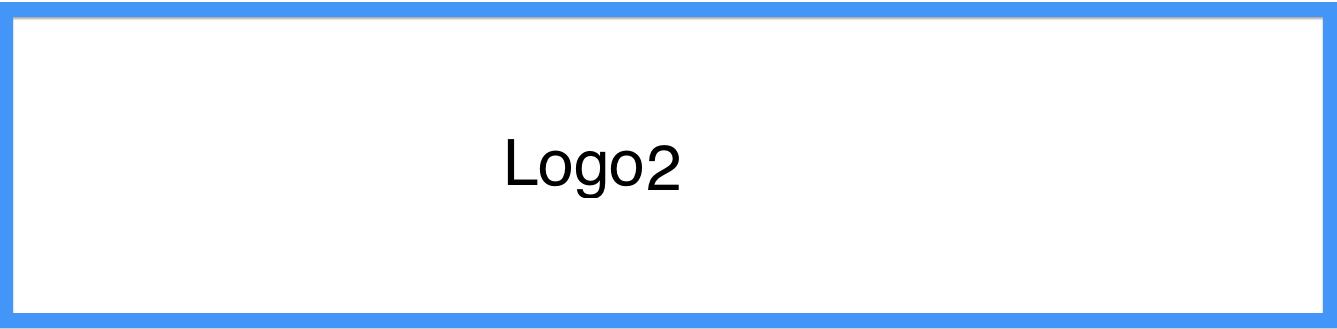
\includegraphics[width=0.3\textwidth]{abb/logo2}
\end{figure}
\vspace{-2cm}

\begin{verbatim}


\end{verbatim}

\begin{center}
\Large{Hochschule der Medien}\\
\Large{Fakultät für Druck und Medien}\\
\end{center}


\begin{center}
\Large{Medieninformatik}
\end{center}
\begin{verbatim}




\end{verbatim}
\begin{center}
\doublespacing
\textbf{\LARGE{\titleDocument}}\\
\singlespacing
\begin{verbatim}

\end{verbatim}
\textbf{{~\subjectDocument}}
\end{center}
%\begin{verbatim}\end{verbatim}
%\begin{center}\end{center}\begin{verbatim}\end{verbatim}
\begin{center}
\textbf{zur Erlangung des akademischen Grades \\ Bachelor of Science}
\end{center}
\begin{verbatim}






\end{verbatim}
\begin{flushleft}
\begin{tabular}{llll}
\textbf{Thema:} & & Deep Reinforcement Learning & \\
& &  \\
\textbf{Autor:} & & Nicolas Reinhart - nr034@hdm-stuttgart.de& \\
& & MatNr. 30038 & \\
& & \\
\textbf{Version vom:} & & \today &\\
& & \\
\textbf{1. Betreuer:} & & Prof. Dr.-Ing. Johannes Maucher &\\
\textbf{2. Betreuer:} & & M.Sc. Johannes Theodoridis &\\
\end{tabular}
\end{flushleft}


% römische Numerierung
\pagenumbering{arabic}

% 1.5 facher Zeilenabstand
\onehalfspacing

% Sperrvermerk
%\section*{Sperrvermerk}
\textcolor{red}{
Die vorliegende Arbeit beinhaltet interne und vertrauliche Informationen der Firma <Firmenname>.
Die Weitergabe des Inhalts der Arbeit im Gesamten oder in Teilen sowie das Anfertigen
von Kopien oder Abschriften - auch in digitaler Form - sind grundsätzlich untersagt.
Ausnahmen bedürfen der schriftlichen Genehmigung der Firma <Firmenname>.
}


%\newpage

% Einleitung / Abstract


%\section*{Zusammenfassung}
%&Hier steht der Text, welcher den Inhalte der Arbeit zusammenfasst...


\section*{Abstract}
\pagestyle{empty}
Heutzutage sind für viele Reinforcement Learning Benchmark-Umgebungen, wie Gym \cite{brockman2016openAI_gym} von openAI der Goldstandard. Das Team von Procgen, ebenfalls von openAI, ging noch einen Schritt weiter und implementiert für einige der Atari Spiele eine prozedurale Generierung der Level. Das allein führt bei einigen Algorithmen bereits zu besserer Sample Efficiency und einer besseren Generalisierung. 

In dieser Arbeit wird untersucht, wie sich eine visuelle Augmentation der Environments im Training oder während der Evaluation auf den allgemeinen Erfolg, den Reward und die Generalisierung auswirkt. Experimente mit maskierten Informationen oder invertierter Semantik untersuchen darüberhinaus die Relevanz bestimmter visueller Informationen und die Generalisierung von Konzepten.
Durchgeführt werden die Experimente im Chaser-Environment von Procgen. Dieses Spiel ist angelehnt an den Atari-Klassiker \dq Ms. Pac-Man\dq. Wie im Original ist es das Ziel, alle Orbs einzusammeln und auf dem Weg nicht von den Geistern gefressen zu werden.

Die Experimente der vorliegenden Arbeit zur farblichen Änderungen des Environments zeigen, dass bspw. die Existenz einer gewissen Farbe für die Erkennung eines Objekts große Relevanz besitzt, wenn das Objekt diese Farbe im Training hat. So nimmt die Performance eines Agenten rapide ab, wenn die Farbe der Orbs in der Evaluation eine andere ist, verglichen mit der zu Trainingsbedingungen. Des Weiteren zeigt sich über die Arbeit hinweg immer wieder, dass die Änderungen der Evaluationsumgebung und die daraus resultierenden Änderungen der Pixel-Verteilung, welche der Agent als Input bekommt, ebenfalls fatale Auswirkungen auf die Performance des Agenten haben. 

Experimente mit Änderung der Semantik von Objekten zwischen Training und Evaluation zeigen eindeutig, dass das der Architektur vorangestellte Convolutional Neural Network (CNN) stark auf die optische Erscheinung der Objekte fixiert ist. Das Vertauschen zweier Sprites stellt eine unüberwindbare Hürde für den Agenten dar. Die Feature Extraction des CNN scheint stark auf die Texturen und die Formen der jeweiligen Objekte angewiesen zu sein, um diese korrekt zu erkennen. So scheut sich der Agent, bei Experimenten mit invertierter Semantik der großen Orbs und der Geister, einen statischen Gegner einzusammeln - ein großen Orb, welcher ihn mit den Bewegungen eines Geistes verfolgt, wird hingegen gedankenlos eingesammelt. 


% einfacher Zeilenabstand
\singlespacing

% Inhaltsverzeichnis anzeigen
\newpage
\tableofcontents

% das Abbildungsverzeichnis
\newpage
% Abbildungsverzeichnis soll im Inhaltsverzeichnis auftauchen
\addcontentsline{toc}{section}{Abbildungsverzeichnis}
% Verion 1: Abbildungsverzeichnis MIT führender Nummberierung endgueltig anzeigen
\listoffigures

% Verion 2: Abbildungsverzeichnis OHNE führende Nummberierung endgueltig anzeigen
%\begingroup
%\renewcommand\numberline[1]{}
%\listoffigures
%\endgroup


% das Tabellenverzeichnis
%\newpage
% Tabellenverzeichnis soll im Inhaltsverzeichnis auftauchen
\addcontentsline{toc}{section}{Tabellenverzeichnis}
% \fancyhead[L]{Abbildungsverzeichnis / Abkürzungsverzeichnis} %Kopfzeile links
% Tabellenverzeichnis endgültig anzeigen
\listoftables

%% WORKAROUND für Listings
%\makeatletter% --> De-TeX-FAQ
%\renewcommand*{\lstlistoflistings}{%
%  \begingroup
%    \if@twocolumn
%      \@restonecoltrue\onecolumn
%    \else
%      \@restonecolfalse
%    \fi
%    \lol@heading
%    \setlength{\parskip}{\z@}%
%    \setlength{\parindent}{\z@}%
%    \setlength{\parfillskip}{\z@ \@plus 1fil}%
%    \@starttoc{lol}%
%    \if@restonecol\twocolumn\fi
%  \endgroup
%}
%\makeatother% --> \makeatletter
% das Listingverzeichnis
%\newpage
% Listingverzeichnis soll im Inhaltsverzeichnis auftauchen
%\addcontentsline{toc}{section}{Listingverzeichnis}
%\fancyhead[L]{Abbildungs- / Tabellen- / Listingverzeichnis} %Kopfzeile links
%\renewcommand{\lstlistlistingname}{Listingverzeichnis}
%\lstlistoflistings
%%%%

% das Abkürzungsverzeichnis
% Abkürzungsverzeichnis soll im Inhaltsverzeichnis auftauchen
\addcontentsline{toc}{section}{Abkürzungsverzeichnis}
% das Abkürzungsverzeichnis entgültige Ausgeben
\fancyhead[L]{Abkürzungsverzeichnis} %Kopfzeile links
%\nomenclature{UGC}{User Generated Content}

\nomenclature{ALE}{Atari Learning Environment}
\nomenclature{RL}{Reinforcement Learning}
\nomenclature{DRL}{Deep Reinforcement Learning}
\nomenclature{GPU}{Graphical Processing Unit}
\nomenclature{MDP}{Markov Decision Process}
\nomenclature{POMDP}{Partially Observable Markov Decision Process}
\nomenclature{SLP}{Single Layer Perceptron}
\nomenclature{MLP}{Multi Layer Perceptron}
\nomenclature{NN}{Neuronales Netzwerk}
\nomenclature{IHPfPVG}{Investigating Human Priors for Playing Video Games}
\nomenclature{SW}{Sliding Window}
\nomenclature{PCG}{Prozeduraler Content Generierung}
\nomenclature{KI}{Künstliche Intelligenz}
\nomenclature{MSE}{Mean-Squared-Error}
\nomenclature{FFN}{Feed Forward Netzwerk}
\nomenclature{CNN}{Convolutional Neural Network}
\nomenclature{SW}{Sliding Window}
\nomenclature{DNN}{Deep Neural Network}
%\nomenclature{}{}


\printnomenclature[3cm]


%%%%%%% EINLEITUNG %%%%%%%%%%%%
\newpage
\fancyhead[L]{\nouppercase{\leftmark}} %Kopfzeile links

% 1,5 facher Zeilenabstand
\onehalfspacing

% einzelne Abschnitte
\section{Einleitung \& Motivation}\label{einleitung}
\pagestyle{fancy}
%\setcounter{page}{1}
Die Forschung rund um Reinforcement Learning (RL) hat in den letzten Jahren stark an Interesse gewonnen. Eine Suche des Begriffs ‘Reinforcement Learning’ auf Google trends zeigt, dass sich die Häufigkeit der Anfragen dieses Begriffs seit 2016 knapp verdreifacht hat.
Gegenwärtige Benchmark-Umgebungen wie openAI’s Gym \cite{brockman2016openAI_gym} helfen den Fortschritt in der Forschung weiter voranzutreiben. Ein Weiterer, häufig verwendeter Simulator ist das Atari Learning Environment (ALE) \cite{bellemare2013arcade}. Das ALE bietet signifikante Forschungs-Aufgaben für RL, model-learning, model-based planning, imitation learning, transfer learning und intrinsic motivation \cite{bellemare2013arcade}. Neben den Vorteilen, die eine solche Benchmark-Umgebung und die darin befindlichen Atari Spiele mit sich bringen, haben diese Umgebungen immer noch entscheidende Nachteile: Die Level in einigen dieser Umgebungen sind händisch erstellt worden. Somit gibt es nur eine begrenzte Anzahl an Szenarien, in denen trainiert werden kann. Dieser Fakt führt bei der Arbeit mit RL-Agenten oft zu schlechterer Generalisierung und instabilen Policies \cite{zhang2018natural}.
Das Framework von Procgen adressiert das Problem der Generalisierung durch prozedurale Erstellung der Spielumgebung. Der prozedurale Anteil steuert dabei Entscheidungen wie die Logik des Levellayouts, die Position und Spawn-Zeiten von Spielelementen, die Auswahl der Game-Assets und weitere \cite{cobbe2019procgen}.

Im Paper \cite{dubey2018investigating} untersuchen die Autoren, warum Menschen im Lösen komplexer Videospiele so gut sind. Genauer untersuchen sie die Rolle von Vorwissen, welches hilfreich scheint, um eine schnelle und effiziente Exploration eines Frames oder eines Levels zu ermöglichen. Die Arbeit der Autoren dient als grundlegende Inspiration für diese Arbeit. Über den Verlauf ihrer Experimente hinweg verändern sie die visuelle Darstellung ihres Spiels bis zu einem Punkt, an dem bspw. die Ähnlichkeit von gleichen Objekten vollständig maskiert ist. Die in der Arbeit \cite{dubey2018investigating} erstellten Level werden von Menschen und einem RL-Agenten gespielt und ihre Leistungen werden verglichen. Die Level für den Agenten sind aufgrund der Komplexität des gewählten Spiels vereinfacht.

In der vorliegenden Arbeit wird untersucht, wie sich visuelle Augmentation des Environments auf die durch Procgen geförderte Generalisierung und den allgemeinen Erfolg trainierter Agenten auswirkt. Hierfür wird ein Environment von Procgen mit dem Titel \emph{Chaser} \cite{cobbe2019procgen}~[S.15 A.6] herangezogen. Dieses Spiel stellt ein Replika des Atari-Klassikers \dq Ms. Pac-Man\dq{} dar. 

Die Experimente sind in drei verschiedene Sets eingeteilt. Das erste Set überprüft die Reproduzierbarkeit der Ergebnisse aus dem Procgen-Paper und untersucht die Auswirkung prozeduraler Level-Generierung auf die Performance eines Agenten.

Das zweite Set beschäftigt sich mit visuellen Veränderungen der Farbe der Orbs und des Hintergrundes (BG), aber auch mit der Maskierung von Information, die im Training gegeben war. So werden in diesem Set z.B. Agenten in der Evaluation mit Herausforderungen konfrontiert wie: die Farbe der Orbs ist eine andere, als im Training oder die Orbs werden überhaupt nicht dargestellt.

Das dritte Set befasst sich ausschließlich mit der semantischen Invertierung von visueller Information unterschiedlicher Spielelemente. Hierbei werden bspw. in der Evaluation die Sprites von kleinen Orbs und Mauern oder großen Orbs und Gegnern vertauscht und somit die Semantik optisch invertiert. Ein Bild des Environments kann Abbildung \ref{fig:pic_chaserGros} entnommen werden. Kleine Orbs sind hier in grün und große sind gelb. Die Gegner sind die grünen Blobs mit drei Stacheln. Die Mauern sind grau. Diese Abbildung zeigt das Spiel in seiner unveränderten Form. 

Die ausgeführten Experimente finden in Anlehnung an die in \cite{dubey2018investigating} durchgeführten Experimenten statt. Besonders Änderungen der visuellen Semantik und die daraus resultierende Änderung der Erscheinung von Objekten, sollte die verwendete IMPALA-Architektur \cite{espeholt2018impala}, aufgrund des vorangeschaltenen CNN, vor komplexe Aufgaben stellen. 


\paragraph{Ziel der Arbeit}\label{ziel_der_arbeit}
Ziel dieser Arbeit ist die Untersuchung der Generalisierung des eingesetzten IMPALA-Netzwerks \ref{absch_setup_impala} im Zusammenspiel mit dem verwendeten PPO Algorithmus \ref{absch_RL_ppo},in der Procgen-Umgebung \cite{cobbe2019procgen}. Dies geschieht anhand unterschiedlicher visueller Augmentationen des Trainings- und/oder der Evaluations-Environments. Genauer wird die durch Procgen \ref{absch_EXP_procgen} geförderte Generalisierung in ungesehenen Leveln untersucht. Die Evaluation ist anhand vorab erstellter Fragen realisiert. Diese geschieht unter Verwendung zweier visueller Veränderungen des Agenten-Inputs, während des Trainings und/oder der Evaluation: farbliche Änderungen von Spielelementen wie bspw. der Orbs und visuell-semantische Invertierung von zwei unterschiedlichen Spielelementen. \\
Diese Experimente folgen drei Sets an Fragen, welche in Kapitel \ref{subsec_EXP_durch_fragen} ausführlich aufgelistet sind. 

In den Experimenten des Unterkapitels \ref{absch_EXP_durch_serie1} wird Data Augmentation in Form von farblicher Änderung oder optischer Maskierung mancher Spielelemente betrieben. Hiermit wird einerseits durch optische Maskierung untersucht, wie relevant gewisse Objekte des Environments, hier die kleinen Orbs, für einen erfolgreichen Abschluss einer Episode sind. Andererseits wird mittels farblicher Änderungen untersucht, ob während des Trainings eine Konzeptualisierung der kleinen Orbs stattfindet. Mit einem ausreichenden Konzept eines kleinen Orbs, sollten farbliche Änderungen des Orbs in der Evaluation zu keinem Verlust der Performance führen. Zudem wird untersucht, ob mehrere Level innerhalb einer kleinen Anzahl an Zeitschritten auswendig gelernt werden können, und wie relevant die visuelle Information der kleinen Orbs dabei ist.

Die Experimente in Unterkapitel \ref{absch_EXP_durch_serie2} untersuchen, wie ein trainierter Agent in der Evaluation abschneidet, wenn Spielelemente, wie die großen Orbs und die Geister, auf visuelle Weise semantisch invertiert sind. Hierbei wird untersucht, ob während der Feature Extraction auch nicht-optische Features, wie bspw. ein Bewegungsmuster, ein Indikator für ein Spielelement sein kann. Des Weiteren wird durch eine Invertierung der kleinen Orbs und der Mauern überprüft, ob ein Agent ein Grundverständnis des Spiels aufweist, oder ob er dadurch auf die Leistung eines Random-Agenten zurückfällt. 

Das erste erwähnte Set an Fragen \ref{subsec_EXP_durch_fragen} beschäftigt sich mit der Reproduktion der Ergebnisse der Arbeit \cite{cobbe2019procgen} und der generellen Auswirkung der prozeduralen Level-Generierung und schafft lediglich das Fundament der folgenden Experimente.\\



Kapitel \ref{hauptabschnitt_2} beschreibt die verwandten Arbeiten, welche für die vorliegende Arbeit als Inspiration dienen oder technisch relevant sind. Das dritte Kapitel (\ref{hauptabschnitt_3}) legt die theoretische Grundlage für die Arbeit dar. Hier wird unter anderem der PPO Algorithmus und die IMPALA-Architektur erläutert. Das Kapitel \ref{hauptabschnitt_4} befasst sich mit dem Setup der Experimente. Hier wird das Environment beschrieben und seine Eigenschaften erläutert. Kapitel \ref{hauptabschnitt_5} handelt von der Durchführung der Experimente. Wie zuvor erwähnt, sind die Experimente in Sets unterteilt. Diese Sets werden systematisch mit Experimenten untersucht. Das sechste Kapitel (\ref{ausblick}) gibt eine Ausblick über offene oder während der Bearbeitung des Themas aufgekommene Fragen und mögliche Abläufe für Experimente, um diese zu untersuchen. Kapitel \ref{konklusion} fasst die Arbeit abschließend zusammen und beschreibt die Erkenntnisse, welche aus den Experimenten gewonnen werden können. 


\newpage

\section{Verwandte Arbeiten}\label{hauptabschnitt_2}
%PROZEDURAL GEN



%AUGMENTATION
%DIESER ANFANG EVENTUELL INS ABSTERACT AUFNEHMEN
Das Problem des Overfittings ist in der Welt des Machine Learnings weit verbreitet. RL hat die generelle Problematik, dass Agenten oft schlecht  generalisieren und somit innerhalb ihrer Trainingsumgebung zwar gute Leistungen erbringen, außerhalb jedoch nicht (\cite{cobbe2019procgen}, \cite{zhang2018study}). Diese Arbeit verwendet die Ansätze der prozeduralen Generierung und der Data Augmentation, um das Problem der Generalisierung zu untersuchen.

%##########################################
%##########################################
%PROZEDURAL
%\paragraph{par:ha2_procGen} 
Die Idee von Procedural Content Generation (PCG) ist kein neuer Ansatz. Die Spieleindustrie macht sich die Eigenschaften von PCG bereits Ende der achtziger Jahre in \dq Dungeons \& Dragons\dq{} zu nutze. Durch die Anwendung von PCG in der Domäne Künstlicher Intelligenz (KI), kann die Generalisierung und Sample Efficiency in einigen Environments bereits stark verbessert werden. So war openAI mit Hilfe von PCG in der Lage, eine ausreichend große Level-Anzahl und Diversität bereitzustellen, um das Spiel \dq Capture the Flag\dq{} zu meistern. Weiter schaffen die Autoren es ebenso, dass die Spieler eines Teams in Kooperation arbeiten \cite{jaderberg2019human}. Inzwischen ist die Verwendung von PCG zur künstlichen Erweiterung der Trainingsumgebung bzw. des Trainingsdatensets eine etablierte Alternative zum händischen Erweitern. Arbeiten wie \cite{risi2019procedural} oder \cite{risi2019increasing}, beide von Sebastian Risi und Julian Togelius, zeigen die mögliche Anwendung für KI und Herrausforderungen, die dabei zu beachten sind. 
Die hier aufgeführten Arbeiten stützen die These, dass eine prozedurale Erstellung des Trainingsenvironments positive Auswirkungen auf die Generalisierung hat. Die Experimente in \ref{sec:absch_EXP_durch_reproduktion} und \ref{subsec:absch_EXP_durch_reproduktion_generalisierung}, sowie einige Experimente in Unterkapitel \ref{absch_EXP_durch_serie1} liefern empirische Beweise für die positive Auswirkung.
%##########################################
%##########################################

%##########################################
%##########################################
%DATA AUGMENTATION
%\paragraph{par:ha2_dataAug} 
Data Augmentation wird typischerweise im Supervised Learning eingesetzt. Arbeiten wie \cite{geirhos2018imagenet} zeigen, welche Erfolge mittels künstlicher visueller Erweiterung eines bereits vorhandenen Datensatzes erzielt werden können. Die Autoren erweitern das \emph{ImageNet} \cite{imagenet_cvpr09} zu ihrem eigenen \emph{Stylized ImageNet}. In ihrer Arbeit zeigen sie, dass das eingesetzte CNN, im Fall des ImageNets, Texturen mit größerem Fokus als Formen lernen. Um diese Einseitigkeit zu verbessern, fügt ihre Optimierung dem zugrunde liegenden Datensatz bspw. Bilder hinzu, bei denen Texturen anderer Bilder auf die vorhandenen Bilder multipliziert sind. Was danach vom eigentlichen Bild übrig ist, sind lediglich die Form und die Kontraststufen. Das Training auf den erweiterten Daten resultiert in einer \dq  [...] improved object detection performance and previously unseen robustness towards a wide range of image distortions, highlighting advantages of a shape-based representation\dq{}  \cite{geirhos2018imagenet}[S. 1] \footnote{\label{foot:absch_RL_mdp_ubersetzung}Übersetzung des Verfassers: verbesserten Leistungen bei Bilderkennung und bisher ungesehen Robustheit bezüglich einer weiten Spanne an verschiedenen Bildverzerrungen, was auf die Vorteile von formbasierter Repräsentation hinweist.}. Diese Arbeit ist nur ein Beispiel für die Empfindlichkeit von CNNs gegenüber optischer Änderung. Ein weiteres Beispiel liefert die Arbeit \cite{reith2019convolutional}. Hier untersuchen die Autoren anhand spezifischer, optischer Stimuli, welche Muster potentiell besser erkannt werden können, als andere. 
Auch die Verwendung von Data Augmentation in RL ist nicht neu. Die Arbeit \cite{raileanu2020automatic} untersucht die Auswirkungen verschiedener Arten von visuellen Augmentationen und erzielt mit ihrem Ansatz in den 16 Environments von Procgen eine bessere Performance um bis zu ca. 40\%.  Auch ältere Arbeiten, wie \cite{zhang2018natural}, sind ein Beleg für die Relevanz von Data Augmentation in RL. 

Die in dieser Arbeit durchgeführten Experimente sind grundlegend durch die Arbeit \cite{dubey2018investigating} und die darin behandelten Experimente inspiriert. In der Arbeit werden die Auswirkungen von Vorwissen des Menschen auf die Performance, die der Mensch in einem Spiel erbringen kann, gemessen und mit einem RL-Agenten verglichen. Darüber hinaus testen sie die Kenntnis grundlegender Interaktionen mit Gegenständen, wie bspw. einer Leiter. So wird in dieser Arbeit das Sprite der Leiter durch ein einfarbiges Bild ersetzt, welches dieselben x- und y-Dimensionen wie das Bild der Leiter hat. Hierdurch soll die Semantik und Identität des Objekts maskiert werden. Ebenso haben sie die Semantik von zwei Objekten vertauscht. Das Bild der Leiter wird dann bspw. durch ein Bild aus mehreren kleinen Flammen ersetzt. Die Herausforderungen, die dem Menschen gestellt wurden, wurden in abgewandelter Form ebenfalls dem RL-Agenten gestellt. Hier ist die These, dass visuelle Änderungen, die Menschen vor eine schwierige Aufgabe stellen, für einen RL-Agenten, welcher mit der Situation im Training konfrontiert wurde, keine Rolle spielen, da er über keinerlei Vorwissen verfügt. Die von den Autoren aufgestellte These stellt sich nach ihrer Auswertung als wahr heraus. Die Experimente der Arbeit \cite{dubey2018investigating} bieten Potential herauszufinden, wie relevant gewisse visuelle Stimuli für den Agenten sind. So lässt sich bspw. mittels visueller Maskierung mancher Spielelemente testen, wie relevant diese Information für den Abschluss eines Environments sind. 

%In einer Arbeit von Amy Zhang, Yuxin Wu und Joelle Pineau \cite{zhang2018natural} wird bspw. der Hintergrund von Atari-Spielen durch verschiedenste Videos der realen Welt ersetzt. Das Hinzufügen der natürlichen Diversität realer Umgebungen soll zur Generalisierung beitragen. 


%Arbeiten wie \cite{kostrikov2020image} bedienen sich Techniken der klassischen Augmentation, wie sie aus dem Bereich Computer Vision bekannt sind. Erweiterungen wie das Abschneiden außen liegender Teile des Bildes, rotieren, grau-skalieren oder mit Farben multiplizieren und Random Noise alleine, führen schon zu verbesserter Generalisierung und teilweise zu besserer Sample Efficiency. 
%##########################################
%##########################################



\newpage

\section{Deep Reinforcement Learning - Theorie}\label{hauptabschnitt_3}
Das wissenschaftliche Feld des maschinellen Lernens bietet viele verschiedene Ansätze einem Agenten beizubringen, wie er eine gegebene Aufgabe bewältigt. Dieses Feld lässt sich in drei Gruppen einteilen: Supervised Learning, Unsupervised Learning und \emph{Reinforcement Learning} (RL). RL differenziert sich von den anderen beiden Feldern durch die fehlenden Trainingsdaten. In diesem Feld werden die Trainingsdaten mittels Interaktionen in einem Environment gesampled. RL ist ein facettenreiches Forschungsfeld. Es vereint Anwendungen aus bspw. der Kontrolltheorie, dem maschinellen Lernen und weiteren Feldern in Einem. RL ist inspiriert durch den Ansatz des verstärkenden Lernens der Verhaltenspsychologie. Im Folgenden werden die für diese Arbeit benötigten Grundlagen eingeführt.


\subsection{Markov Decision Process}\label{absch_RL_mdp}
Der \emph{Markov Decision Process} (MDP) \cite{mdp_bellman} stellt ein mathematisches Framework für das Problem des Lernens durch Interaktion dar. 
Das Framework stellt die Rahmenbedingungen, in einem diskreten, stochastischen und sequenziellen Environment zielorientierte Entscheidungen zu treffen. Hierzu wird die gesamte Interaktion zwischen dem Agenten und dem Environment auf drei Signale reduziert. Ein \emph{State} ist hierbei der Zustand des Environments und beschreibt alle Übergangswahrscheinlichkeiten. Der Agent fällt seine Entscheidung auf Basis dieses States. Mittels \emph{Actions} kann der Agent mit dem Environment interagieren und dessen State verändern. Für die Ausführung einer Action erhält der Agent einen \emph{Reward} und den nächsten State. Der Reward stellt die Belohnung dar und kann sowohl positiv als auch negativ sein. Das Ziel des Agenten ist es, möglichst zielführende Actions auszuwählen und damit seinen Reward zu maximieren.

Dieser Prozess ist eine Erweiterung des \emph{Markov Reward Process} um die Fähigkeit Entscheidungen zu treffen. MDPs bieten die Möglichkeit Entscheidungen selbst in Situationen zu treffen, in denen der Ausgang nicht zu 100 \% von den Aktionen des Agenten abhängt, sondern durch Zufall verfälscht wird. Dem Agenten steht dabei die Teilmenge $A(s) \subset A $, die Menge aller möglichen Aktionen in State $s \in S$ zur Verfügung. Eine generelle Formulierung eines MDP deckt die meisten RL-Probleme ab und besteht aus dem folgenden Tupel $\langle S, A, P, R, \gamma \rangle$: 

\begin{itemize}
  \item $S$ ein Set aus States 
  \item $A$ ein Set aus Actions
  \item $P$ Übergangswahrscheinlichkeiten $P_{ss'}^a = \mathbb{P}[s_{t+1} = s' | s_t = S, a_t = A]$
  \item $R$ eine Reward-Funktion $R_s^a = \mathbb{E}[R_{t+1} | s_t = S, a_t = A]$
  \item $\gamma$ ein Diskontierungsfaktor $\gamma \in [0,1]$
  \begin{itemize}
     \item $\gamma$ = 0 => Monte-Carlo (Aktionswahl nur anhand des aktuellen States)
     \item $\gamma$ = 1 => $TD(1)$ (Aktionswahl anhand aller möglichen Folgestates)
  \end{itemize}
 % \item $Q(s,a)$ Action-Value Function $Q_{\pi}(s,a) = \mathbb{E}[G_t | S_t = s, A_t = a]$
  \label{lst:itemList_mdp}
\end{itemize}

\begin{figure}[htb]
 \centering
 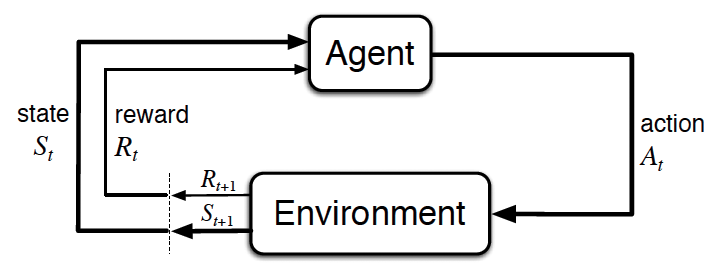
\includegraphics[width=0.3\textwidth,angle=0,scale=2.5]{abb/mdp_EnvLoop}
 \caption[Beschreibung]{Visualisierung des RL Prozesses mittels eines MDP \cite{sutton2011reinforcement}~[S.38]}
\label{fig:fig_mdpEnvLoop}
\end{figure}

Abbildung \ref{fig:fig_mdpEnvLoop} beschreibt die Interaktionen in einem MDP. Der Agent interagiert mit dem Environment für eine diskrete Anzahl an Schritten $t = 1, 2, 3, ..$. Am Anfang eines jeden Schrittes $t$ wählt der Agent eine Aktion $a_t$ und erhält daraufhin einen nummerischen Reward $R_{t+1} \in R \subset \mathbb{R}$ und den Folgestate $s_{t+1}$.

Während man im Markov Reward Prozess versucht die Action-Value Function $ Q_*(a) $ einer jeden Action zu schätzen, berechnet man in einem MDP die State-Action Value Function $ Q_*(s,a) $ einer jeden Action in jedem State oder man schätzt den Value eines States $ V_*(s) $. Bei der Berechnung des Values mittels $ V_*(s) $, wird eine optimale Auswahl der Actions vorausgesetzt. Ein Sternchen im Index steht hier repräsentativ für die optimale Policy. Der Index der Funktionen $ V_{\pi} $ und $Q_{\pi}$ referenziert folgend auf die aktuell verfolgte Policy. Die State-Value Function $V$ kann dabei als Dekomposition, in Form eines Erwartungswerts des aktuellen Rewards $ R_{t+1} $ und des diskontinuierten Values des Folge-States $ V(s_{t+1}) $, formuliert werden.


\begin{quotation}
\centering
   \( V_{\pi}(s) = \mathbb{E}_{\pi} [ R_{t+1} + \gamma V_{\pi}(S_{t+1}) | s_t = S ]  \) 
\end{quotation}


Die State-Action-Value Function $Q$ kann auf ähnliche Weise formuliert werden. Diese Funktion schätzt, wie gut eine Action $a$ unter der Prämisse ist, dass der Agent sich im State $ s_t $ befindet. 


\begin{quotation}
\centering
   \( Q_{\pi}(s,a) = \mathbb{E}_{\pi} [ R_{t+1} + \gamma Q_{\pi}(S_{t+1}, A_{t+1}) | s_t = S, a_t = A ]  \) 
   \label{eq:q_estimate}
\end{quotation}


Das Verhalten des Agenten kann, innerhalb des durch den MDP gegebenen Rahmens, als Policy $\pi(a|s)$ definiert werden, wobei $\pi $ eine Wahrscheinlichkeitsverteilung über alle States mit allen Actions darstellt. Diese Verteilung kann wie folgt definiert werden: 


\begin{quotation}
\centering
\( \pi(a|s) = \mathbb{P}_{t}[a_t = A | s_t = S] \label{eq:mdp_policy} \). %\footnote{Silver, vgl. \cite{silverCourse_mdp}~[S.26]}
\label{eq:mdp_policy}
\end{quotation}


Das beste Verhalten für ein gegebenes Problem  zu finden, bedeutet analog die Policy $\pi$ zu finden, die den Erwartungswert des akkumulierten diskontinuierten Rewards, über die Schritte $t$ hinweg, maximiert. Der Return $G_t$ ist der totale, diskontinuierte Reward und wird durch die folgende Gleichung definiert:

\begin{quotation}
\centering
   \( G_t = R_{t+1} + \gamma R_{t+2} + \gamma^{2} R_{t+3} + ... = \sum\limits_{k=0}^{\infty} \gamma^k R_{t+k+1} \) \footnote{Sutton und Barto, vgl. \cite{sutton2011reinforcement}~[S.44] } \label{eq:mdp_return}.
\end{quotation}


%$\mathbb{R} \rightarrow$ [0,1] mit $F(t) = P (X \le t)$ heißt Verteilungsfunktion von $X$



\subsection{Deep Learning}\label{absch_RL_deepL}
Im Gegensatz zu einem \emph{Single Layer Perceptron} (SLP), enthält ein \emph{Multi Layer Perceptron} (MLP) verborgene Schichten zwischen der Eingabe- und der Ausgabeschicht. Die verborgenen Schichten sind die sogenannten Hidden-Layers, von denen es beliebig viele hintereinander geben kann. Die Anordnung von mehreren Hidden-Layers von Neuronen, ist inspiriert vom biologischen Informations-Verarbeitungs-Prozess des menschlichen Gehirns. Da die verborgenen Layers nicht direkt mit der Ausgabe zusammenhängen, werden sie Hidden-Layer genannt \cite{Goodfellow-et-al-2016}[S. 164-165]. 

Ein Deep Neural Network (DNN) zielt darauf ab, Schicht für Schicht, aus einfachen Inputs wie bspw. einem Vektor aus Zahlen oder einem Pixel-Stream, informative Features zu extrahieren. Abbildung \ref{fig:maucher_dnn} zeigt eine abstrakte Darstellung eines DNN. Was ein einfaches MLP von einem vollwertigen DNN differenziert ist die Extraktion der Features (orange in Abb. \ref{fig:maucher_dnn}), die im Deep Learning dem Netzwerk überlassen ist. Diese Features müssen somit nicht manuell extrahiert werden. Der blaue Teil der Abbildung (\ref{fig:maucher_dnn}) ist applikations-spezifisch und könnte statt einem Classifier bspw. durch ein Regressionsmodell ersetzt werden. Die automatisierte Feature Extraction ermöglicht es eine Architektur auf unterschiedliche Probleme anzuwenden. Das ist möglich, da kein domänen-spezifisches Vorwissen mehr nötig ist, um dem applikations-spezifischen Teil des Netzwerks informative Features bereitzustellen. Die Verbindungen zwischen den Neuronen der jeweiligen Layer sind, wie bei einem SLP oder einem MLP, gerichtet und gewichtet. In der Feature Extraction befinden sich typischerweise Layer wie Convolutional-, Pooling-, RNN-, LSTM- und Attention-Layers. Der Teil des Classifier wird oft mit einem einfachen SLP oder einem mehrschichtigen MLP realisiert, bestehend aus Dense-Layers oder Fully-Connected-Layers.
\begin{figure}[htb!]
 \centering
 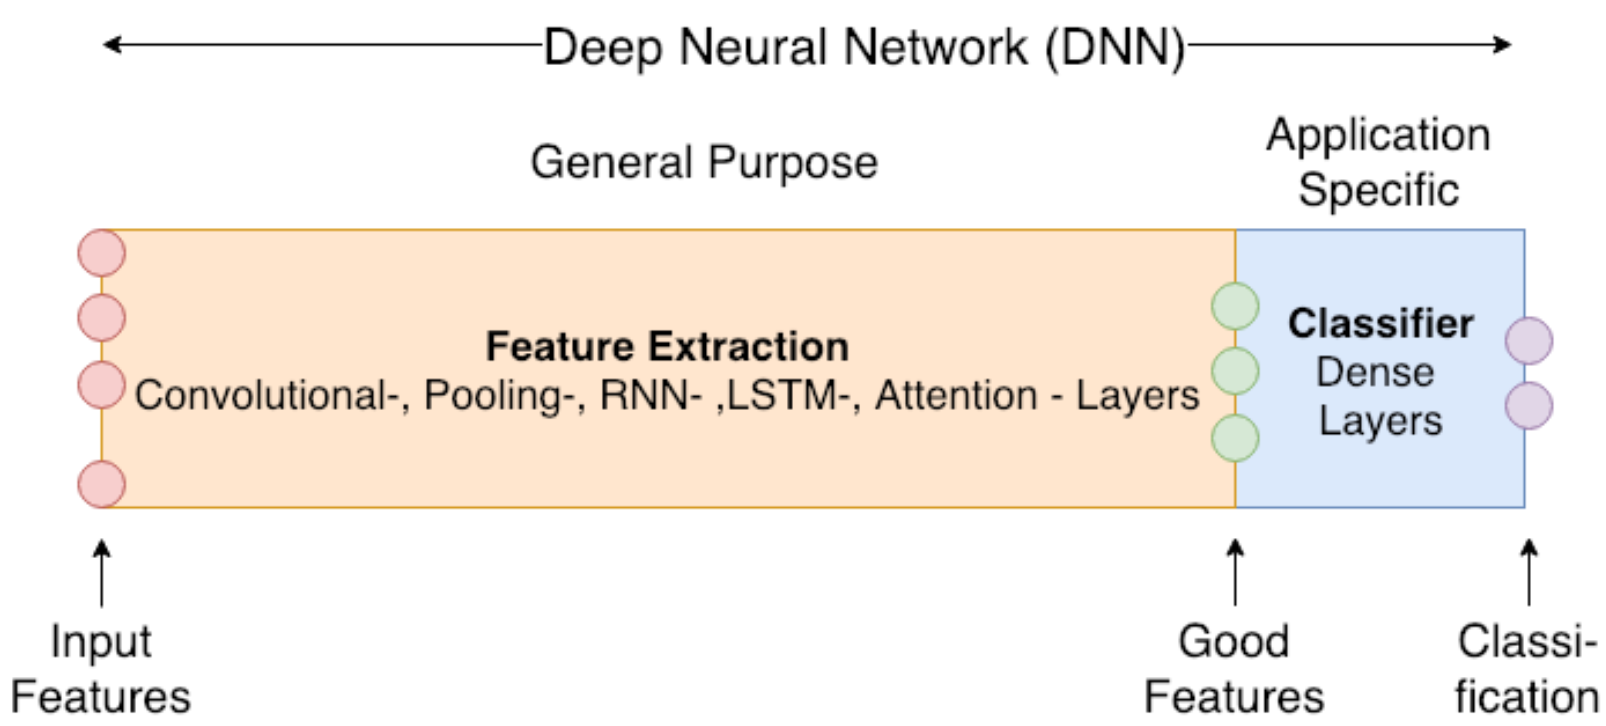
\includegraphics[scale=0.34]{abb/maucher_dnn}
 \caption[Beschreibung]{Abstrakte Darstellung eines DNN \cite{maucher_nb_cnn}. }
\label{fig:maucher_dnn}
\end{figure}
\newline

Viele Problemstellungen, wie das Verarbeiten eines Pixel-Streams, sind sehr komplex. Ein Frame eines Spiels von 60 auf 60 Pixeln, aufgeteilt in drei Farbkanäle, ergibt eine Anzahl von 10.800 Datenpunkten, die verarbeitet werden müssen. Anders als bei einem einfachem SLP oder einem MLP werden beim Deep Learning Entscheidungen nicht direkt abhängig vom Input getroffen. Hier werden über mehrere Abstraktions-Layer hinweg, nicht-lineare Anpassungen an den Daten vorgenommen. Eine ausführliche Motivation für tiefe Architekturen gibt die Arbeit \cite{bengio2009learning} von Yoshua Bengio.

Aufgrund der großen Anzahl an Neuronen sind die tiefen Neural Networks (NN) in der Lage komplexe Problemstellungen, wie aus einem Pixel-Stream eine Action abzuleiten, die in dieser Situation Reward-steigernd erscheint, auszuwählen. Im Bereich Deep Q-Learning wird bspw. die Approximation der State-Action-Value Function $Q(s,a)$, mit einem NN realisiert. Das State-Action-Value NN approximiert dann bspw. im Training den erwarteten durchschnittlichen Reward des übergebenen States-Action Tupels $(s,a)$ und wird typischerweise anhand des TD-Errors \ref{TD-Error} oder des Mean-Squared-Errors (MSE) \footnote{\label{foot:absch_RL_deepL_mse} Der MSE ist die Summe, der quadrierte Differenz zwischen tatsächlichen Wert $x(i)$ und der Vorhersage $\hat{x}(i)$ , geteilt durch die Anzahl an Datenpunkten. $MSE =  \frac{1}{n} \sum \limits_{i=1}^n ( x( i ) - \hat{x}(i))^2 $ } zum tatsächlich erhaltenen Return hin korrigiert. 



\subsubsection{Deep Feedforward Netzwerke}\label{absch_RL_deepL_FFN}
Deep \emph{Feedforward Networks} (FFN) sind die Basis des Deep Learnings. Ziel einer solch tiefen Architektur ist es, eine Funktion zu approximieren. So mapped ein solches Netzwerk, im Falle eines Classifiers, ein Eingabebild $x$ zu einem Label $y$. Das Mapping von Bild zu Label ist definiert durch $y = f(x,w)$, wobei $w$ die Gewichte darstellt, die es zu lernen gilt. Diese werden optimiert, um die bestmögliche Approximation von $f(x)$ zu ermöglichen. Der Name der FFN definiert den Informationsfluss. So haben FFNs, im Vergleich zu bspw. rekurrenten Netzwerken, ausschließlich vorwärts gerichtete Verbindungen - daher die Bezeichnung feedforward. Diese Grundarchitektur stellt die Basis vieler Anwendungen, wie CNNs dar. CNNs sind lediglich eine spezielle Form eines FFNs. Solche Netzwerke werden durch azyklische Graphen beschrieben, welche definieren, wie die approximierende Funktion zusammengesetzt ist. Hat man bspw. ein Netzwerk mit drei Schichten, so besteht dieses aus drei verschiedenen Funktionen, die wie folgt miteinander verkettet sind: 

\begin{quotation}
\centering
   \( f(x) = f^3 (f^2 ( f^1 (x))) \)
\end{quotation}

In diesem Fall stellt $f^1$ den ersten Layer dar, $f^2$ den zweiten, usw. Die gesamte Länge der Verkettung gibt die Tiefe des Netzwerks an. Der letzte Layer ist mit dem Output des Netzwerks verbunden. Ein repräsentatives Bild der Verkettung in Form eines MLP der Tiefe $L=3$ kann dem Anhang entnommen werden (\ref{anh_mlp_L3}). Die Eingabeschicht wird hierbei nicht zur Tiefe des Netzwerks gezählt. 

Während des Trainings werden die Parameter des gesamten Netzwerks so verändert, dass sich die Funktion $f(x)$ an die optimale Approximation $f_*(x)$ annähert. Jedes Element des Trainings $x$ muss also im Output-Layer möglichst genau das korrekte Label $y$ produzieren. Wie die Layer zwischen Input und Output korrigiert werden, um näher an $f_*(x)$ zu gelangen, wird über den angewandten Lernalgorithmus definiert.

Eine tiefe FFN-Architektur könnte wie folgt sein: Am Netzwerk liegt der Input, bspw. ein eindimensionaler Vektor, an. Dieser Vektor wird dann durch eine Serie an Hidden-Layers, bis hin zum Output-Layer transformiert. Jeder Hidden-Layer besteht aus mehreren Neuronen, die vollständig mit den Neuronen des vorherigen und nachfolgenden Layers verbunden sind. Neuronen in Hidden-Layers teilen hier keine Verbindungen untereinander und agieren unabhängig voneinander. Der eben beschriebene Teil der Architektur übernimmt die Feature Extraction. Der letzte vollständig verbundene Layer entspricht dem Output-Layer. Im Fall von Klassifikationen würden im Output-Layer die Scores für die jeweiligen Klassen stehen, bspw. 10 Outputs bei 10 verschiedenen Klassen. 



\subsection{Convolutional Neural Networks}\label{absch_RL_convNets}
CNNs sind seit mehreren Jahren etabliert im Einsatz für Objekt-Detektion, Objekt-Erkennung, Sprach-Erkennung und weitere. Diese Netzwerke sind eine spezialisierte Form der in Unterkapitel \ref{absch_RL_deepL_FFN} vorgestellten FFNs. Ebenso wie FFNs bestehen CNNs oft aus sehr vielen Schichten an Neuronen, mit Gewichten, die es zu lernen gilt. Der größte Unterschied zwischen FFNs und CNNs besteht in der Verwendung der Convolutional-Layer bzw. in der Anwendung von Convolutional Filtering. Diese Layer sind darauf ausgelegt lokale Informationen, bspw. aus benachbarten Pixeln aus Bildern oder umgebenden Wörtern in einem Text in ein Feature zu extrahieren. Aufbauend auf der Annahme, dass die umgebende Region für eine betrachtete Stelle relevant ist, teilen sich die Neuronen dieser Region die Gewichte zum nachfolgenden Neuron. Durch die many-to-one-Beziehung sind CNNs in der Lage, komplexe Inputs wie ein Bild zu verarbeiten. CNNs lernen damit automatisch häufig vorkommende Merkmale der Trainingsdaten, welche für den applikations-spezifischen Teil der Architektur relevant sind. 
 
Die Bilder des Datensatzes \emph{CIFAR-10} \footnote{\label{foot:absch_RL_CNN_CIFAR10} Der Datensatz von CIFAR-10 beinhaltet 60.000, $32*32$ Farbbilder, eingeteilt in 10 Klassen.} \cite{cifar10_krizhevsky} sind bspw. $32*32$ Pixel groß und haben drei Farbkanäle (RGB). Damit hat der ersten Convolutional-Layer einen Input von $32*32*3 = 3.072$ Datenpunkten. Im Fall dieser Arbeit wird bereits mit doppelt so großen Frames, ebenfalls mit drei Farbkanälen gearbeitet ($64*64*3 = 12.288$). Auch diese Größe ist noch weit von einem brauchbaren Bild entfernt, wie Abbildungen \ref{fig:pic_chaserGros} und \ref{fig:pic_chaserKlein} zeigen. Eine einfache FFN-Architektur benötigt für ein solches Bild, je nach Aufbau, sehr viele Gewichte und ist deshalb ungeeignet, um direkt mit solchem Input zu interagieren. Convolutional-Layer verbinden Regionen von Neuronen des vorangegangenen Layers mit einem Neuron des Convolutional-Layers. Diese Layer bieten durch die Feature Extraction aus Regionen eine effiziente Reduktion des vorangegangenen Layers. Eine Veranschaulichung dieses Konzepts bezüglich des Netzwerks, bei zweidimensionalem Input, ist im Anhang gegeben (\ref{anh_conv2d}).

CNNs für die Farbbild-Verarbeitung haben im Unterschied zu FFNs, ebenso wie ihr Input, einen dreidimensionalen Aufbau - die Neuronen werden in Höhe, Breite und Tiefe organisiert. Die Breite und die Höhe stehen hierbei für die räumlichen Informationen und die Tiefe für die Anzahl der Farbkanäle des anliegenden Bildes. So bestehen Convolutional-Layer in diesem Fall nicht aus einfachen Neuronen-Schicht, sondern aus einem dreidimensionalen Volumen an Neuronen. 

Typischerweise bestehen CNNs aus drei verschiedenen Layern: Convolutional-Layer, Pooling-Layer und Fully-Connected-Layer. Die einzelnen Layer sind folgend detaillierter erläutert. 


 % \item Input: Dieser ist im Fall von CIFAR-10 ein Bild der Größe $32*32$, mit drei Farbkanälen. 
\textbf{Convolutional:} Diese Layer berechnen den Output aus den lokalen Regionen des Inputs. Sei $(r \times c)$ der zweidimensionale Input, bspw. ein Schwarz-Weiß-Bild, wobei $r$ die X- und $c$ die Y-Koordinate eines Pixels angibt. So gibt $r*c$ die Größe des Bildes an. Weiter sei $(a \times b)$ ein Filter, mit der \emph{Kernel Size} $a*b$, wobei der Filter kleiner als der Input ist. Dieser Filter wird von oben links, bis unten rechts über den Input geschoben. Hierbei wird bei jeder Iteration das Skalarprodukt zwischen den jeweiligen Koeffizienten der Region des Inputs und den Koeffizienten des Filters errechnet. Dieses Skalarprodukt wird nach Anwendung der Aktivierungsfunktion $g$ in den folgenden Layer geschrieben. Ist der geschriebene Wert positiv bedeutet dies, dass das Feature, welches durch die verwendeten Filter repräsentiert wird, vorhanden ist. Ist der Wert $0$ kommt dieses Feature nicht an dieser Stelle des Inputs vor. Der \emph{Stride} entscheidet dabei wie weit der Filter nach jeder Operation bewegt wird. Bei einem Stride von $s=1$ ergeben sich $(r-a+1) * (c-b+1)$ mögliche Positionen für den Filter. Allgemein ist der Output im zweidimensionalen Fall von der Größe $[(r-a+s) \times (c-b+s)]$. Ein Bild dieses Ablaufs kann dem Anhang entnommen werden (\ref{anh_convConcept}). Dieses Bild zeigt einen Input der Größe $[10 \times 10]$ und einen Filter der Größe $[3 \times 3]$. Mit einem Stride von $s=1$ ergibt sich als Ausgabe dieser Operationen ein Layer der Größe $[8 \times 8]$ ($~[(10-3+1) \times (10-3+1)]~$). 
Der Stride des Filters kann auch größer als $1$ sein. Zudem gibt es die Option, dass man dem Bild ein sogenanntes \emph{Padding} hinzufügt oder nicht. Für das Padding gibt es wiederum selbst verschiedene Optionen für die Realisierung. Im Falle der Anwendung von Padding errechnet sich die Größe der Ausgabe bei der Größe des Padding $p$ und bei quadratischem Input und Filter wie folgt: 
\begin{quotation}
\centering
   \( p = \frac{r-a+2p}{s} + 1  \) 
\end{quotation}


\textbf{Pooling:} Ein Pooling-Layer komprimiert die Daten entlang der räumlichen Achsen. Ähnlich wie beim Convolutional-Layer gibt es beim Pooling-Layer eine Art Filter. Dieser Filter verschiebt sich um den Wert des Strides. Bei diesem Filter werden die betroffenen Elemente jedoch nicht aufsummiert, sondern die Koeffizienten, welche der Filter abdeckt, werden mit dem Max-Operator auf einen reduziert. So wird bspw. aus der Ausgabe eines Layers mit $[32 \times 32 \times 10]$, mittels eines Filters der Größe $[2 \times 2]$ und einem Stride von 2 die Ausgabe des Pooling-Layers mit $[16 \times 16 \times 10]$ erzeugt.

\textbf{Fully-Connected:} Dieser Layer errechnet die Scores für die jeweiligen Klassen. Im Fall von zehn Klassen ist das Resultat ein Volumen der Maße $[1 \times 1 \times 10]$ \footnote{Die Ausgabe des vorangehenden Layers wird typischerweise zu einem eindimensionalen Vektor gestaucht. So ergibt sich aus einen Layer der Größe $[2 \times 2]$ ein Vektor der Größe $[1 \times 4]$.}. Bis hier sind die räumlichen Informationen des Bildes vollständig transformiert und übrig bleibt ein quasi eindimensionaler Vektor mit den zehn Klassen-Scores des CIFAR-10 Datensatzes.

\textbf{Activation:} Die Funktion $g$ realisiert eine elementweise Aktivierungsfunktion auf den oben beschriebenen Skalarprodukten. 

Mögliche nicht-lineare Aktivierungsfunktionen der Neuronen: 
  \begin{itemize}
  	\item Sigmoid: $g(x) = \frac{1}{1+e^{-x}}$
  	\item Hyperbolischer Tangens: $g(x) = \frac{1- e^{-2x}}{1+e^{-2x}}$
  	\item ReLU: $g(x) = max(0,x)$ 
  	\item etc.
\end{itemize}


%\cite{krizhevsky2012ConvImageClass}
%\cite{yamashita2018convMedUse}
%CNN's s 




\subsection{Deep Reinforcement Learning}\label{absch_RL_deepRL}
In Deep Reinforcement Learning werden die Policy oder die State-Value Function oder beide zusammen mit einem tiefen NN realisiert. Das hat den Vorteil, dass bspw. das Mapping der State-Action-Value Function $Q$ beim Q-Learning nicht mehr in einer zweidimensionalen Tabelle gespeichert wird. Hier übernimmt das Mapping von State-Action Tupel zu Value ein tiefes NN. Das spart einerseits Anforderungen an die Hardware und kann andererseits schneller eine Antwort liefern, da keine mit der Problemgröße wachsende Tabelle durchsucht werden muss. 

\paragraph{on-policy vs. off-policy}\label{onVSoff-Policy}
Folgend wird der Unterschied zwischen \emph{on-policy}- und \emph{off-policy}-Verfahren erläutert. Beide Verfahren, sowohl \emph{on-policy}, wie auch \emph{off-policy} aktualisieren ihre Schätzungen der Q-Werte anhand des Tupels $(s',a')$. Der Folgestate ist $s'$ und die dann gewählte Action ist $a'$. Die Verfahren unterscheiden sich in der Annahme für die Wahl der folgenden Action $a'$ des Tupels. \newline
\textbf{on-policy:} Diese Verfahren gehen davon aus, dass die Action $a'$ mit der aktuell verfolgten Policy $\pi_t$, zum Zeitpunkt $t$ ausgewählt wird. SARSA ist bspw. ein on-policy-Verfahren.\newline
\textbf{off-policy:} Bei diesem Verfahren wird davon ausgegangen, dass die Action-Wahl \emph{greedy}\footnote{Eine greedy Wahl der Action nimmt immer die Action, welche den höchsten totalen geschätzten Reward verspricht.} getroffen wird. Aus diesem Grund ist Q-Learning ein off-policy Verfahren.

In on-policy geschehen Updates also anhand einer Action-Wahl der aktuell verfolgten Policy. In off-policy wird davon ausgegangen, dass die Action-Wahl einer greedy Policy folgt und somit nicht der aktuell verfolgten Policy entspricht.


\subsubsection{Function Approximation}\label{subsub:absch_RL_deepL_funcAppr}
Im Rahmen dieser Arbeit werden sowohl die Policy, als auch die Value Function mit einem tiefen NN approximiert. 

\paragraph{Value Function Approximation} 
Die State-Value Function $V$ mapped einen State $s$ auf einen Value. Das NN ist mit dem Vektor $w$ parametrisiert. $V(s,w)$ approximiert damit die tatsächliche State-Value Function $V_{*}(s)$. Typischerweise ist die Dimensionalität des Vektors $|w|$ geringer, als die Anzahl an möglichen States $|S|$. Die Reduktion des Problems von der Anzahl an möglichen States auf die Anzahl an verwendeten Gewichten ermöglicht das agieren in komplexen kontinuierlichen Environments. Das Netzwerk wird in Richtung des approximierten erwarteten Returns ($R_{t+1} + \gamma V(S_{t+1}$), bekannt als das \emph{TD Target}, korrigiert. Die Größe eines Updates von $V$ wird mittels des Hyperparameters $\alpha$ kontrolliert. 

\begin{quotation}
\centering
   \( V(s_t) \leftarrow V(s_t) + \alpha(R_{t+1} + \gamma V_{t+1} - V(s_t)) \) \\
\end{quotation} 
Ein Update der State-Action-Value Function $Q$ erfolgt analog. 

\begin{quotation}
\centering
   \( Q(s_t, a_t) \leftarrow Q(s_t, a_t) + \alpha(R_{t+1} + \gamma Q(s_{t+1}, a_{t+1}) - Q(s_t, a_t)) \) \\
\end{quotation}
 Der Estimator der State-Value Function ist wie folgt definiert:

\begin{quotation}
\centering
   \( V_w (s) = \mathbb{E}_{\pi} [ \sum\limits_{k = 0} \gamma^k R_{t+k+1} | s_t = S ] \) \footnote{Der Exponent k steht für die Anzahl der Episoden.}. \\
\end{quotation}
Der Iterator $k$ ist limitiert über die Anzahl an Schritten, die vorausgeschaut werden. Bei $TD(\lambda)$ gibt $\lambda$ diese Anzahl vor. Da man am Ende einer Episode den tatsächlich erhaltenen Reward vom Environment bekommt, ist dieser Teil ein Supervised Learning Problem und kann auch ebenso optimiert werden. 

\paragraph{Policy Approximation}
Policy Gradient Methoden zielen darauf ab, eine Policy direkt aus der Interaktion mit dem Environment zu modellieren und optimieren. Typischerweise wird die Policy ebenfalls als parametrisierte Funktion $\pi_{\theta}(a|s)$ mit den Parametern $\theta$ formuliert. Der resultierende Value der Objectiv Function ist somit abhängig von der verfolgten Policy $\pi$. Die Reward- bzw. Objectiv Function wird definiert durch folgende Gleichung:

\begin{quotation}
\centering
   \(\ J(\theta) = \sum\limits_{s \in S} d^{\pi_{\theta}}(s) V^{\pi_{\theta}}(s)  =  \sum\limits_{s \in S} d^{\pi_{\theta}}(s) \sum\limits_{a \in A} \pi_{\theta}(a|s) Q^{\pi_{\theta}}(s,a)   \) , \\
% Formel von 
% https://lilianweng.github.io/lil-log/2018/04/08/policy-gradient-algorithms.html#what-is-policy-gradient
\end{quotation}
wobei $d^{\pi}(s)$ die Verteilung der makrov'schen Kette für die Policy $\pi_{\theta}$ darstellt. Mittels des Gradienten Aufstiegsverfahrens wird $\theta$ in die Richtung gelenkt, die der Gradient $\bigtriangledown_{\theta}J(\theta)$ vorschlägt, um die erwarteten Rewards zu maximieren.

Das Policy Gradient Theorem legt das theoretische Fundament für die Umformung des Gradienten $ \bigtriangledown J(\theta) $ zu einem Estimator $\mathbb{E}$. \footnote{ Sutton und Barto geben in Sektion 13.2 \cite{sutton2011reinforcement}{S. 268} den Beweis für den episodischen Fall. }

\begin{quotation}
\centering
   \( \bigtriangledown J(\theta)  =  \mathbb{E}_{\pi_{\theta}} [ \bigtriangledown log \pi_{\theta}(a | s, \theta) Q^{\pi_{\theta}}(s,a) ] \) 
\end{quotation}

$ \pi_{\theta} $ ist eine stochastische Policy und $ Q^{\pi_{\theta}} $ ist der State-Action Value Funciton Estimator.


\paragraph{Advantage}\label{subsubsec_RL_advantage}
Um die Varianz im Training zu verringern, wird statt der lediglich value-based Methoden, häufig die Advantage Function eingesetzt und statt der Value Function im Policy Gradient verwendet \cite{schulman2017proximal}. 
Der Advantage ist definiert wie folgt: 

\begin{quotation}
\label{Advantage-Estimate}
\centering
   \(  A(s,a) = Q_b(s,a) - V_w(s)  \)
\end{quotation}

$ Q(s,a) $ entspricht dem Q-Value von Action $ a $ im State $s$, $ V(s) $ dem Value des States $ s $.  Ein Nachteil dieser Praxis ist, dass man $ Q $ und $ V $mit zwei unterschiedlichen Parameter-Sets trainieren muss. Dies geht aus den Indizes der vorangegangenen Gleichung hervor. Um die Notwendigkeit von zwei unterschiedlichen Parametrisierungen zu vermeiden, wird häufig die Umformung angewandt, welche den Advantage Function Estimator $ A $ durch einen Estimator des TD-Errors ersetzt. Für die tatsächliche Value Function $ V^{\pi_{\theta}}(s) $ definiert sich der TD-Error $ \delta^{\pi_{\theta}} $ folgendermaßen: 

\begin{quotation}
\label{TD-Error}
\centering
   \(  \delta^{\pi_{\theta}} = r + \gamma V^{\pi_{\theta}}(s') - V^{\pi_{\theta}}(s)  \)
\end{quotation}

Die Definition von $ Q(s) $ (\ref{eq:q_estimate}) entspricht dem aktuellen Reward, plus dem geschätzten, erwarteten und diskontinuierten Value des nächsten States $ s' $.  Der erste Teil des TD-Errors $ ( r + \gamma V^{\pi_{\theta}}(s') ) $, bedingt durch den aktuellen State $s$ und die Action $a$, entspricht somit der State-Action-Value Function $Q$. 
Ersetzt man nun die State-Action-Value Function mit dem ersten Teil des TD-Errors, für die Schätzung der Advantage Function, erhält man folgende Gleichung: 

\begin{quotation}
\centering
   \( \mathbb{E}_{\pi_{\theta}} [ \delta^{\pi_{\theta}} | s,a]  =  \mathbb{E}_{\pi_{\theta}} [ r + \gamma V^{\pi_{\theta}}(s') | s,a ] - V^{\pi_{\theta}}(s) \)
\end{quotation} 

Somit kann man den TD-Error verwenden, um den Policy-Gradienten zu schätzen und man umgeht damit die Notwendigkeit eines extra Netzwerks bzw. Parameter-Sets für $Q$. Da $V^{\pi_{\theta}}(s)$ den Value des aktuellen States repräsentiert, kann dieser Teil außerhalb des Estimators sein. Nun kann der TD-Error verwendet werden, um den Policy Gradienten zu berechnen.  

\begin{quotation}
\centering
   \(  \delta_{\theta}J(\theta)  =  \mathbb{E}_{\pi_{\theta}} [\bigtriangledown_{\theta} log \pi_{\theta}(s, a) \delta^{\pi_{\theta}}]  \)
\end{quotation}


\subsection{Actor Critic}\label{absch_RL_acModel}
Die Ansätze in model-free RL lassen sich grob in drei Gruppen einteilen.
  \begin{itemize}
  	\item Value-basierte Methoden (bspw. Q-Learning und Deep Q-Learning): In diesen Methoden lernt der Agent eine Value Function $V$, welche jedem State oder jedem State-Action Tupel einen Value zuweist. Diese funktionieren zuverlässig in einer Umgebung mit einer endlichen Menge an Actions bzw. States.
  	\item Policy-basierte Methode (bspw. REINFORCE Policy Gradient): Hier lernt der Agent direkt eine Policy $\pi$, ohne dabei eine State-Value Function zu nutzen. Diese Methoden sind besonders stark in Bereichen, in denen das Environment einen stochastischen oder kontinuierlichen Action Space aufweist.
  	\item Hybrid Methoden (Actor Critic): Diese Methodik vereint die zuvor erwähnten Ansätze zu einem, welcher sowohl eine Value Function einsetzt als auch eine Policy verwendet. Aufgeteilt auf zwei NNs approximiert der Critic eine Value Function, welche den Aktor korrigiert. Diese Methodik vereint die Vorteile der beiden vorherigen Ansätze. Das Training eines Actor Critic Modells generiert seine Samples typischerweise on-policy (\ref{onVSoff-Policy}). Im Fall einer synchronisierten Batched \emph{Advantage Actor Critic} (A2C) Implementierung generiert der Aktor eine Anzahl an Samples $T$, wobei $T$ deutlich kleiner als die Episodenlänge ist. Daraufhin evaluiert der Critic die Samples, aktualisiert seine Schätzungen für die Values der jeweiligen States und aktualisiert die Policy des Aktors.
  \end{itemize}
In dieser Arbeit wird das Actor Critic Modell verwendet. 

%\subsubsection{Advantage}\label{subsubsec_RL_advantage}




\subsection{Proximal Policy Optimization}\label{absch_RL_ppo}
Der Proximal Policy Optimization (PPO) \cite{schulman2017proximal} Algorithmus ist ein on-policy (\ref{onVSoff-Policy}) Policy Gradient Algorithmus. Im folgenden Unterkapitel wird der in dieser Arbeit verwendete Algorithmus zur Optimierung der Policy vorgestellt. 

Unabhängig von den in dieser Arbeit erwähnten Problemen in RL (\ref{absch_EXP_procgen} Overfitting auf große Datensätze, \ref{par:durch_EXP_vgl_200_unbeschr} Sparse-Reward-Problem), haben on-policy Policy Gradient Methoden oft zwei weitere generelle Probleme. Einerseits besteht das Problem, dass generierte Samples bzw. Batches immer abhängig von der aktuell verfolgten Policy sind. Dadurch erlebt der Agent sich konstant ändernde State- und Reward-Verteilungen, was zu Instabilität im Training führen kann.
Andererseits besteht in RL eine große Sensitivität gegenüber Hyperparameter Tuning. 

Darüberhinaus besteht in RL allgemein die Gefahr zu großer Policy-Updates. Wird bspw. ein Batch, anhand dessen die Policy optimiert werden soll, unter einer zufällig schlechten Policy gesampled, so kann es passieren, dass sich die Policy mit einem Update sehr weit von der aktuell verfolgten Policy $ \pi_{\theta} $ entfernt. Auch wenn die Policy bisher zu keinen schlechten Ergebnissen geführt hat, werden nun ggf. sehr viele gute Eigenschaften der bestehenden Policy revidiert. Daraufhin wird der nächste Batch unter noch schlechteren Umständen gesampled. Solch eine falsche Korrektur der Policy zu kompensieren, kann viele Zeitschritte im Training kosten und ggf. erholt sich die Policy nicht mehr vom ersten Batch, der die Policy in diese Richtung verbessert bzw. verschlechtert hat. Das PPO-Paper \cite{schulman2017proximal} zeigt in Abschnitt $6.1$ Experimente mit unbeschränkten Policies. Diese Experimente liefern einen empirischen Beweis für Schwierigkeiten mit unbeschränkten Updates.

\subsubsection{Hintergrund}\label{absch_RL_PPO_hintergrund}
Der PPO Algorithmus ist maßgeblich durch den Trust Region Policy Optimization (TRPO) Algorithmus \cite{schulman2015trust} inspiriert. 

\paragraph{Trust Region Policy Optimization}\label{par:absch_RL_PPO_hintergrund_TRPO}
Um die Stabilität im Training zu verbessern, verhindert TRPO unter anderem die zuvor erwähnten, zu großen Policy Updates. TRPO löst dieses Problem mittels eines sogenannten \emph{KL-Divergence Constraint}, in der Objectiv Function. Grundsätzlich versucht der Algorithmus Folgendes zu maximieren: 

\begin{quotation}
\centering
   \( L^{TRPO}(\theta) =  \mathbb{E}_t [ \frac{ \pi_{\theta}(a_t | s_t)}{ \pi_{\theta_{old}}(a_t | s_t) } A_t  -  \beta KL [ \pi_{\theta_{old}}( \cdot | s_t), \pi_{\theta}( \cdot | s_t ) ] ] \).
\end{quotation}

Der Teil der Gleichung links ($(\pi_{\theta} / \pi_{\theta_{old}}) A_t$) ist ein Verhältnis zwischen der neuen und der alten Policy, unter Betrachtung desselben State-Action Tupels, multipliziert mit dem Advantage Estimate. Dieser Teil stellt die unbeschränkte Policy-Optimierung. Der Hyperparameter $ \beta$, stellt den sogenannten Penalty Coefficient dar. Dieser entscheidet wie stark das KL-Divergence Constraint beachtet wird. Je größer $ \beta$, desto kleiner ist das resultierende Update. Der Term $ KL [ \pi_{\theta_{old}}( \cdot | s_t), \pi_{\theta}( \cdot | s_t ) ] $  \footnote{Kullback-Leibler-Divergence: $ D_{KL}(\pi_1 || \pi_2)[s] = \sum_{a \in A} \pi_1 (a|s) log \frac{\pi_1 (a|s)}{\pi_2 (a|s)} $} errechnet die Divergenz zwischen der alten und der neuen Policy, in anderen Worten die Entfernung zwischen den zwei Policies. Dies geschieht unter Betrachtung des States $s_t$ und allen möglichen Actions.

\subsubsection{PPOs Clipped Objectiv Funciton}\label{absch_RL_qFunc}
Sei $ r_t(\theta) $ das Verhältnis der Wahrscheinlichkeitsverteilungen $ \pi_{\theta} / \pi_{\theta_{old}} $, sodass $ r_t(\theta_{old}) = 1 $, so beschreibt $ r_t(\theta) A_t $ das unbeschränkte TRPO Objectiv. 

\begin{quotation}
\centering
   \( L^{CPI}(\theta) =  \mathbb{E}_t [ \frac{ \pi_{\theta} (a_t | s_t) }{ \pi_{\theta_{old}} (a_t | s_t) } A_t ] = \mathbb{E}_t [ r_t(\theta) A_t ] \)
\end{quotation}

CPI referenziert hier auf \emph{Conservative Policy Iteration} der Arbeit \cite{kakade2002approximately}. Das unbeschränkte TRPO Objectiv wurde in dieser Arbeit erstmalig vorgestellt. Somit ist $ r_t(\theta) $ größer als $ 1 $, wenn eine Action unter der neuen Policy wahrscheinlicher ist, als unter der alten Policy. Im umgekehrten Fall ist $ r_t( \theta ) $ kleiner als 1. Wie in der letzten Problematik \ref{par:absch_RL_PPO_hintergrund_TRPO}im zweiten Absatz bereits erklärt, kann auch dieses Objectiv zu sehr großen Policy Updates führen. Das Update kann so groß sein, dass die Policy es eventuell nicht mehr kompensieren kann, falls es ein schlechtes Update war. 

PPO greift das Objectiv von TRPO auf, doch beschränkt es sich nicht auf die aufwendig zu berechnende KL-Divergence, sondern clipped es lediglich um den Wert $ 1 \pm \epsilon $. $ \epsilon $ ist ein Hyperparameter, welcher typischerweise $0,2$ ist. Zusammen mit dem Min-Operator kann nun das eigentliche PPO-Objectiv vorgestellt werden. 

\begin{quotation}
\label{PPO-clip-objective}
\centering
   \( L^{CLIP}(\theta) =  \mathbb{E}_t [ min ( r_t(\theta) A_t , clip ( r_t(\theta), 1 + \epsilon, 1 - \epsilon ) A_t ) ] \)
\end{quotation}

Diese Objectiv Function nimmt das Minimum aus zwei Termen. Der erste Term im Min-Operator ($ r_t(\theta) A_t $) ist das unbeschränkte TRPO Objectiv, wie in \ref{absch_RL_PPO_hintergrund} vorgestellt. Der zweite Term beschränkt das Verhältnis $ r_t(\theta) $ auf eine Differenz von $1 \pm \epsilon $ und multipliziert dann mit dem Advantage Estimate, wie in \ref{absch_RL_actorCriticPPO} definiert. Die daraus resultierende Policy $\pi_{\theta}$ kann sich somit, innerhalb eines Updates, nicht weiter als $ \epsilon $ von der alten Policy $ \pi_{\theta_{old}} $ entfernen. 

Der PPO Algorithmus vereinfacht somit das KL-Divergence Constraint zu einer Clip-Operation. Zudem ist eine Schwäche des TRPO, dass es kein $ \beta $ gibt, welches über mehrere Environments hinweg erfolgreich ist. Selbst in einem einzigen Environment kann ein statisches $ \beta $ zu einer schlechten Performance führen. Dieses Problem besteht bei PPO nicht. 

%EVTL INTUITION HINTER DER GLEICHUNG ERKLÄREN. AUCH DIE GRHEN IM PPO PAPER FÜR DEN ADVANTAGE...


\subsubsection{PPO Actor Critic Style}\label{absch_RL_actorCriticPPO}
In dieser Arbeit wird der PPO Algorithmus zusammen mit dem Actor Critic Model verwendet. Folgend wird der \emph{Loss}-Term vorgestellt, welche PPO einsetzt. Im PPO-Paper teilen sich die Netzwerke für die Value Function und die State-Action-Value Function einen großen Teil der Parameter. Genauer teilen sie sich die Object Detection und Feature Extraction. 

In dieser Arbeit sind die Object Detection und Feature Extraction durch das IMPALA-Netzwerk (\ref{absch_setup_impala}) gegeben. Die Architektur teilt sich im Output-Layer in zwei Heads auf. Einen für die Value Function und einen für die Policy. Aufgrund dessen, dass sich die NNs einen großen Teil der Netzwerk-Parameter teilen, kann die gesamte Architektur mittels einer Loss-Term optimiert werden. 

\begin{quotation}
\centering
   \( L_t ^{CLIP+VF+S}(\theta) =  \mathbb{E}_t [L_t ^{CLIP}(\theta) - c_1 L_t ^{VF}(\theta) + c_2 S[\pi_{\theta}](s_t) ] \)
\end{quotation}

Der Term $ L_t ^{CLIP}(\theta) $ stellt dabei das Clipped Objectiv dar, wie in \ref{PPO-clip-objective} definiert. $ L_t ^{VF}(\theta) $ stellt einen Loss-Term dar, welche wie folgt definiert ist:
\begin{quotation}
\centering
   \(  L_t ^{VF}(\theta) = (V_{\theta}(s_t) - V_t ^{targ})^2  \) .
\end{quotation}

$V_{\theta}(s_t)$ ist eine Value Function, wie sie im Abschnitt \ref{subsub:absch_RL_deepL_funcAppr} definiert ist. $V_t ^{targ}$ ist der tatsächliche Return eines Batches. Dieser Term $ L_t ^{VF}(\theta) $ ist somit ein Squared-Error Loss. 

$ S[\pi_{\theta}](s_t) $ ist ein Term, welcher die Entropie der Gleichung erhöht. Durch den Entropie-Term betreibt der Agent im Training anfänglich viel Exploration, bis die anderen Terme der Gleichung ausreichend Gewicht erlangen. Die Koeffizienten $c_1$ und $c_2$ sind Hyperparameter zur Gewichtung der jeweiligen Terme. Optimiert wird dann mit einem stochastischen Gradienten-Abstiegsverfahren.

Der PPO Algorithmus nutzt eine Implementierung, wie sie in \cite{mnih2016asynchronous} dargestellt ist. In dieser Implementierung sampled die Policy für $ T $ Schritte, wobei $T$ deutlich kleiner als die Episodenlänge ist. Anhand dieses Segments wird der Agent aktualisiert. Diese Art des Samplings benötigt jedoch eine Anpassung des Advantage Estimators, da dieser ansonsten Teile der \emph{Trajectory}. Eine Trajectory $\tau_H$ ist ein Pfad des Agenten durch den State Space des Environments bis zum Horizont $H$ beachten würde, welche über T hinaus liegen. Das kleine $t$ spezifiziert hier den aktuellen Zeitschritt in $[0,T]$ und das große $T$ spezifiziert die Länge des Segments. 

\begin{quotation}
\centering
   \( A_t = -V(s_t) + r_t + \gamma r_{t+1} + ... + \gamma^{T-t+1} r_{T-1} + \gamma^{T-t} V(s_T) \)
\end{quotation}

Im Fall von $\lambda = 1$ kann die vorangegangene Gleichung zur folgenden Gleichung vereinfacht werden. $\delta_{t}$ entspricht hierbei dem TD-Error zum Zeitpunkt $t$, wie in \ref{TD-Error} definiert.

\begin{quotation}
\centering
   \( A_t = \delta_t + (\gamma \lambda)\delta_{t+1} + ... + (\gamma \lambda)^{T-t+1} \delta_{T-1} \)
\end{quotation}

\paragraph{Pseudocode PPO}
Die Implementierung des PPO, welcher mit Segmenten von Trajectories konstanter Länge arbeitet, ist folgend als Pseudocode gegeben. Dieser Code geht von einem Fall aus, in welchem man mehrere Aktoren parallel laufen lässt und dann über die Segmente aller Aktoren optimiert. In dieser Arbeit wird jedoch nur mit einem Aktor gearbeitet ($N=1$). 


\begin{algorithm}
\caption{Pseudocode Implementierung des PPO, Actor Critic }
\begin{algorithmic}

\WHILE{$i < iterations $}
	\WHILE{$actor < N$}
		\STATE  run policy $ \pi_{\theta_{old}} $ in environment for T steps 
		\STATE compute advantage estimates $ A_1, ..., A_T$
	\ENDWHILE
	\STATE optimize surrogate objectiv $ L(\theta) $ with K epochs and minibatches of size $ M \leq NT $
	\STATE $ \theta_{old} \leftarrow \theta $
\ENDWHILE

\end{algorithmic}
\end{algorithm}


\subsection{IMPALA Architektur}\label{absch_setup_impala}
Die IMPALA-Architektur wird im Paper \cite{espeholt2018impala} erstmalig vorgestellt. Die Abkürzung IMPALA steht für \textbf{Imp}ortance Weighted \textbf{A}ctor-\textbf{L}earner \textbf{A}rchitecture. Der wichtigste theoretische Beitrag dieses Papers besteht in der Vorstellung einer Möglichkeit zur asynchronen Separation von Aktoren und Lernern. Das ermöglicht es mehreren Aktoren simultan auf unterschiedlichen Maschinen, mit unterschiedlichen Versionen derselben Policy zu trainieren. Nach einer gewissen Anzahl von Episoden schickt der Aktor seine Samples an den Lerner. Der Lerner muss daraufhin, während des Updates, in Betracht ziehen, dass die Samples der Aktoren (ggf. alle) mit unterschiedlichen Policies generiert wurden. Aus dieser Asynchronität folgt, dass der Aktor einen Batch mit einer Policy generiert, welche seit mehreren Versionen obsolet ist. Da ein Update nicht notwendigerweise anhand der aktuellsten Policy geschieht, handelt es sich um ein off-policy Verfahren (\ref{onVSoff-Policy}). Das in der Arbeit \cite{espeholt2018impala} beschriebene off-policy Actor-Critic Verfahren wird von den Autoren \emph{V-trace} genannt. Eine genaue Definition ist in Kapitel 4 der Arbeit \cite{espeholt2018impala} gegeben.

Wie bereits in \ref{absch_RL_actorCriticPPO} erwähnt, wird in dieser Arbeit nur mit einem Aktor trainiert. Was aus der Arbeit \cite{espeholt2018impala} übernommen wird, ist die Netzwerk-Architektur mit geteiltem Object Recognition Layer und der Trennung in zwei unterschiedliche Heads. Im Vergleich zum Paper ist die Architektur für diese Arbeit mit dem Faktor $4$ skaliert. Das bedeutet, dass die Architektur vier mal breiter ist, als die im Paper. Die Tiefe des Netzwerks wird durch die Skalierung nicht verändert. Ein Bild des Object Recognition Layers kann dem Anhang entnommen werden (\ref{anh_impala_arch}).



%\cite{espeholt2018impala}
%Dieses Paper enthält eine brauchbare Grafik zum erläutern der Impala architektur
%\cite{espeholt2019seed}











\newpage

\section{Experimente - Setup}\label{hauptabschnitt_4}

Alle Experimente wurden mit der Implementierung von baselines (openAI \cite{openai_baselines_code}) realisiert. Das eingesetzte Set an Hyperparametern und die verwendete Hardware kann dem Anhang entnommen werden (Hyperparameter \ref{hyperparameter}, Hardware \ref{hardware})

\subsection{Procgen Benchmark Umgebung}\label{absch_EXP_procgen}
Ein generelles Problem in RL sind die zugrunde liegenden Daten bzw. die verwendeten Environments. Eine Studie von Zhan, Vinyal, Munos und Bengio \cite{zhang2018study} zeigt, dass Agenten selbst auf großen Trainings-Sets overfitten können. Dieses Problem wird durch die prozedurale Generierung in Procgen \cite{cobbe2019procgen} adressiert. So wird die Fähigkeit des Agenten zu Generalisieren ein wichtiger Bestandteil einer erfolgreichen Policy, wobei dieser durch den theoretisch endlosen, prozedural erzeugten Level-Stream gefördert wird. Weiter fördert Procgen durch die hohe Diversität der einzelnen Level ebenfalls die Sample Efficiency. Aus den zuvor beschriebenen Umständen sind die Environments gut geeignet, um Sample Efficiency und Generalisierung zu messen.

Die Procgen Benchmark Umgebung von openAI bietet 16 verschiedene Spiele. Inspiriert von Gym\cite{brockman2016openAI_gym}, ebenfalls von openAI, sind alle Spiele im Retro-Stil. Insgesamt zielt Procgen auf die folgenden Punkte ab: experimenteller Komfort, hohe Diversität innerhalb von Environments und hohe Diversität zwischen Environments \cite{openAI_procgen_blog}. Procgen steht open source zur Verfügung und wurde im Dezember 2019 veröffentlicht. 

\subsection{Chaser}\label{absch_RL_chaser}

\begin{figure}[bp!]

   \captionsetup{width=0.45\linewidth} 
    \centering
    \begin{minipage}{0.45\linewidth}
        \centering
        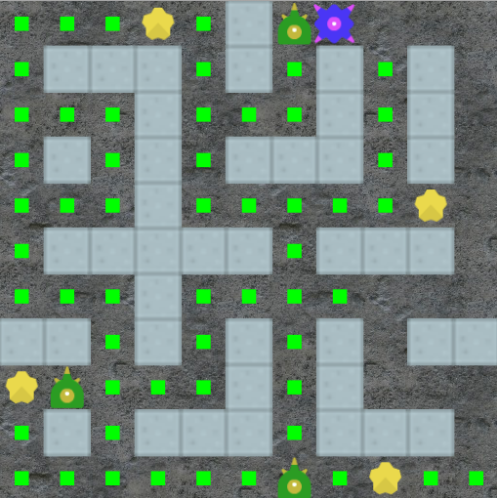
\includegraphics[scale=0.3]{abb/ss_chaser_gros}
        \caption{Chaser - unskaliert.}
        \label{fig:pic_chaserGros}
    \end{minipage}
    %\hfill
    \begin{minipage}{0.45\linewidth}
        \centering
        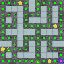
\includegraphics[scale=2.35]{abb/ss_chaser_klein}
        \caption{Chaser - herunterskaliert.}
        \label{fig:pic_chaserKlein}
    \end{minipage}
    %\caption{Chaser Environment - links unskaliert, rechts skaliert}
\end{figure}


Folgend wird das gewählte Spiel Chaser für die Experimente vorgestellt. Ein Bild des Spiels kann Abbildung \ref{fig:pic_chaserGros} entnommen werden. Ein Blick auf den Input des Agenten bietet die Abbildung \ref{fig:pic_chaserKlein}. Dieser ist auf $64 * 64$ Pixel herunter skaliert. 
Das Spiel Chaser ist von dem Atari-Klassier \dq Ms. Pac-Man\dq{} inspiriert. Der Agent spielt den \emph{Jäger}. Ziel des Jägers ist es, alle auf der Karte befindlichen grünen Orbs einzusammeln. Bei Erfüllung des Ziels bekommt der Agent einen hohen extra Reward von 10 Punkten. Zum Vergleich: ein normaler grüner Orb gibt nur einen Reward von 0.04. Unterdessen muss der Agent den drei Geistern ausweichen, die sich im Spiel befinden.

Die Geister können sich in vier verschiedenen States befinden. Diese werden folgend erläutert.
  \begin{itemize}
    	\item \emph{idle-State}: Dieser State ist ein Übergangsstate, in welchem die Geister auf dem Spielfeld erscheinen. Nach $t_1$ Sekunden wird der Geist automatisch in den tödlich-State überführt. Dieser State ist optisch durch ein eigenes Sprite differenziert. Geister in diesem State bewegen sich nicht und können dem Jäger noch nicht schade. 
  	\item \emph{tödlich-State}: Eine Berührung des Jägers mit einem Geist in diesem State beendet die Episode. Die Geister laufen in diesem State zufällig und ziellos. 
  	\item \emph{verletzlich-State}: Geister können vom Jäger in diesem State gefressen werden. Sammelt der Jäger einen großen Orb ein, überführt er die Geister damit in diesen State. Dieser State ist optisch durch ein eigenes Sprite differenziert. Dieser State führt nach $t_2$ Sekunden wieder in den tödlich-State, wenn der Geist nicht gefressen wird.
  	\item \emph{killing-State}: Ist ein Geist zwei oder weniger Felder vom Jäger entfernt, so wird der Geist in diesen State überführt. In diesem State läuft der Geist nicht mehr in zufällige Ricthungen, sondern zielstrebig auf den Jäger zu. 
  \end{itemize}

Der Action Space des Agenten ist diskret und beläuft sich auf 15 Aktionen. Dem Agenten steht dabei die folgende Menge an Actions zur Verfügung: \\ \newline
$ ~ M = \{ \leftarrow, \uparrow, \rightarrow, \downarrow,  \leftarrow + \uparrow, ~ \uparrow + \rightarrow, ~ \rightarrow + \downarrow, ~\downarrow + \leftarrow, ~'stehen~bleiben', W, A, S, D, Q, E \}$. \newline


Diese beinhalten 'stehen bleiben' und 'laufen' in vier Richtungen, mit der Option eine Richtungstaste mit einer daneben liegenden zu kombinieren ($ \leftarrow + \uparrow, ~ \uparrow + \rightarrow, ~ \rightarrow + \downarrow, ~\downarrow + \leftarrow $). Die Kombination aus zwei Richtungstasten führt jeweils zu einer eigenen Action. Bspw. führen die Richtungen 'hoch' $\uparrow$ und 'links' $\leftarrow$ zusammen zur Action 'hoch-links' $\uparrow \leftarrow$. Bewegt sich der Agent bspw. aktuell nach oben und die Action 'hoch-links' ($\leftarrow \uparrow$) wird ausgeführt, so läuft der Agent so lange 'hoch', bis sich die nächste Möglichkeit nach links zu laufen ergibt. Dann läuft er automatisch 'links'. Der Action Space beinhaltet nicht nur die vier Richtungstasten und die Kombinationen nebeneinander liegender Richtungen, sondern auch die Tasten W, A, S, D, Q und E. Hierbei sind die Tasten W, A, S und D gleich belegt wie die Tasten $\uparrow, \leftarrow, \downarrow und \rightarrow$ (in der selben Reihenfolge). Die Tasten Q und E sind gleich belegt wie die Kombinationen $\leftarrow + \uparrow, ~ \uparrow + \rightarrow$. Durch die Redundanz im Action Space mit den Buchstaben-Tasten, lässt sich die Anzahl der möglichen Aktionen von 15 auf 9 reduzieren. Dabei werden die Tasten W, A, S, D, Q und E deaktiviert. Aus Gründen der Vergleichbarkeit zu anderen Arbeiten, wird in dieser Arbeit durchweg mit 15 Actions gearbeitet.


Das Spiel kann in drei verschiedenen Modi gespielt werden. Diese States sind: Easy, Hard und Exploration

\begin{center}
 \begin{table}[htb!]
 \begin{center}
  \begin{tabular}{ l c c c c }
    \hline
     & Easy & Hard & Exploration \\ \hline \hline
     totaler Orb Reward & 0,04 & -1,04 & 1,04 \\ \hline
     extra Orb Reward & 0 & -1 & 1 \\ \hline
     Fertigstellungsbonus & 10 & 10 & 10 \\ \hline
     Spielfeldgröße & 11x11 & 13x13 & 19x19 \\ \hline
    \hline
    %\multicolumn{2}{|c|}{Info in einer Zelle} \\
    %\hline
  \end{tabular}
  \caption{Übersicht über die unterschiedlichen Reward-Settings. Vergabe der Rewards für Orbs ist abhängig vom gewählten Modus.}
  \label{tab:tab_reward_Modi}
  \end{center}
 \end{table}
\end{center} 

Diese unterscheiden sich in der Größe des Spielfelds und im Reward-Systems. Die Vergabe der Rewards durch das Environment ist abhängig vom gewählten Modus und lässt sich in Tabelle \ref{tab:tab_reward_Modi} ablesen. Diese Arbeit verwendet ausschließlich den Modus \emph{Easy}. In jedem Modus sind drei Gegner auf dem Spielfeld. Diese erscheinen jedes Spiel an einer zufälligen Position in unterschiedlichen Quadranten des Spielfeldes. Das Fressen eines Geistes bringt keinen Reward, ebensowenig wie das Gefressen werden.

Der State Space des Environments ist insofern variabel, dass die PCG nicht immer Level mit der selben Anzahl an freien Feldern hervorbringt. Bezogen auf die möglichen Pixel-Verteilungen ergibt sich ein theoretischer State Space von 68,7 Mrd. \footnote{256 Farben pro Farbkanal, drei Farbkanäle, bei einer Bildgröße von 64 auf 64 Pixel. ($256^3 * 64 * 64 = 68.719.476.736$)} möglichen States. Jedoch ist diese Zahl nicht die tatsächliche Größe des State Spaces, da die Berechnung der 68,7 Mrd. auf der Annahme stützt, dass jedes Pixel jede mögliche Farbe annehmen kann. Durch den Algorithmus der Level-Erstellung und die Verwendung von Sprites wird die Zahl deutlich reduziert. 

Das Layout des Levels wird mit prozeduraler Generierung erstellt. Mit Hilfe des Kruskal Algorithmus \cite{kruskal1956shortest}~[S.48-50] wird ein Spanning Tree über das Spielfeld gelegt, welcher alle Felder miteinander verbindet. Daraufhin werden so lange Wände entfernt, bis keine toten Enden mehr unter den Pfaden sind. Das Environment ist deterministisch, bis auf die Geister im tödlich-State. In diesem State bewegen sich die Geister zufällig durch das Level. Formal gesehen entspricht das Environment somit einem POMDP \cite{astrom1965optimal}.

Aufgrund des hohen Rewards von $10$ für den letzten eingesammelten Orb, kann davon ausgegangen werden, dass ein Agent mit einem durchschnittlichen Reward $ \geq 10$ in der Evaluation erfolgreich besteht. Erreicht ein Agent in der Evaluation eines Checkpoint bspw. einen durchschnittlichen Reward $\geq 10$, so kann man sagen, dass der Agent in der Evaluation besteht. 

%\subsubsection{Hintergrund}\label{absch_RL_hintergrund}




\newpage

\section{Experimente - Durchführung}\label{hauptabschnitt_5}
\paragraph{Motivation}\label{par_EXP_durch_motiv}

Die in Kapitel \ref{hauptabschnitt_2} erwähnten Experimente der Arbeit \cite{dubey2018investigating} bieten unausgeschöpftes Potential zur Evaluation der Generalisierung eines RL-Agenten. So kann bspw. durch die Maskierung der Information der Orbs getestet werden, wie wichtig diese Information für den erfolgreichen Abschluss eines Levels ist. Darüber hinaus kann man damit ermitteln, ob der Agent etwas über die zugrunde liegende Level-Struktur bzw. den Algorithmus der die Level erstellt, lernt oder das gesamte Konzept des Spiels verstanden hat. Darüberhinaus wird untersucht, ob die Orbs dem Agenten nach einer gewissen Trainings-Dauer keinerlei wichtige Information mehr bieten. 

Viele DRL-Agenten, die im Rahmen von Arcade-Spielen eingesetzt werden, bekommen den Bildschirm-Output des jeweiligen Spiels in Form eines ein- oder zwei-dimensionalen Arrays als Input. Somit ist alles was der Agent bisher an Stimuli erhalten hat lediglich ein Array mit ein oder zwei Dimensionen. Nimmt man nun in einer Evaluation Änderungen am Environment vor, kann das radikale Auswirkungen auf die Performance des Agenten haben. 


\subsection{Zu beantwortende Fragen}\label{subsec_EXP_durch_fragen}
Unter den bisher beschriebenen Umständen wurden für diese Arbeit folgende Sets an Fragen entwickelt, die über den Verlauf der Experimente beantwortet werden. \\
Das erste Set reproduziert die Ergebnisse aus dem Procgen-Paper \cite{cobbe2019procgen} und untersucht die Auswirkung von prozeduraler Level-Erstellung auf die Performance von Agenten. Dieses Set dient hauptsächlich der Bestätigung der Korrektheit der Implementierung.\\
Das zweite Set befasst sich mit visuellen Veränderungen der Farbe der Orbs und des Hintergrundes, aber auch mit Maskierungen gewisser visueller Information. \\
Das dritte Set befasst sich ausschließlich mit semantischen Veränderungen, wie das Tauschen von zwei Sprites.

\paragraph{Set 1 - Reproduktion und Generalisierung}\label{par_EXP_durch_fragen1}
\begin{itemize}
  \item Lassen sich die Ergebnisse aus dem Paper \cite{cobbe2019procgen} mit den eingesetzten Mitteln reproduzieren?
  \item Wie wirkt sich die prozedurale Erstellung und die daraus folgende hohe Diversität der Level auf die Generalisierung und die Sample Efficiency aus?
  \label{lst:itemList_EXP_durch_fragen1}
\end{itemize}
\paragraph{Set 2 - Farbliche Änderung}\label{par_EXP_durch_fragen2}
 \begin{itemize}
  %\item Wie wirkt sich die prozedurale Erstellung und die daraus folgende hohe Diversität der Level auf die Generalisierung und die sample efficiency aus?
  \item Wie wirkt sich das Fehlen visueller Orb-Information auf die Performance aus? 
  \item Wurde das Konzept eines Orbs verstanden? Wirken sich Änderungen der Farbe der Orbs negativ aus? 
  \item Wie viele Level können mit der verwendeten Architektur auswendig gelernt werden? Welche Rolle spielt die visuelle Orb-Information dabei? 
  \label{lst:itemList_EXP_durch_fragen2}
\end{itemize}

\paragraph{Set 3 - Semantische Invertierung}\label{par_EXP_durch_fragen3}
\begin{itemize}
  \item Wie wirkt sich das Tauschen der Sprites von kleinen Orbs und Mauern aus?
  \item Wie wirkt sich das Tauschen der Sprites von großen Orbs und Geistern aus? \\ 
  \label{lst:itemList_EXP_durch_fragen3}
\end{itemize} 

Das genau Setup bezüglich Dauer des Trainings oder Anzahl der trainierten Level etc. ist tabellarisch bei den jeweiligen Experimenten definiert. 
Generell wird die Leistung der Agenten mit einer \dq one-shot\dq -Evaluation bewertet. Das bedeutet, dass die Episode, während der Evaluation eines Levels, keine Zeitbeschränkung hat und kein Level ein zweites Mal dran kommt. Weiter wird standardmäßig auf 50 unbekannten Leveln trainiert. Änderungen an diesem Vorhaben werden in den jeweiligen Experimenten erläutert. Die Abkürzung SW steht folgend für Sliding Window. 

\paragraph{Farbliche Distanz}\label{farblicheDistanz}
Fortan definiert der Begriff der \emph{farblichen Distanz} die Entfernung zweier Farben zueinander, in einem dreidimensionalen Farbraum. Diese Distanz misst also die absolute Differenz der jeweiligen RGB-Farben. So haben die Farben Rot (r:255, g0:, b:0) und die Farbe Blau (r:0, g0:, b:255) eine farbliche Distanz von $510$. Von rot zu blau muss der Rot-Wert der Farbe auf $0$ und der Blau-Wert auf $255$ gesetzt werden ($|-255| + |255| = 510$). So ergibt sich für die Farben Schwarz und Weiß eine farbliche Distanz von $765$.

\subsection{Reproduktion der Ergebnisse von Procgen}\label{sec:absch_EXP_durch_reproduktion}
Bevor die Experimente der jeweiligen Sets evaluiert werden können, muss die Frage beantwortet sein, ob die verwendeten Implementierungen in der Lage sind, die Ergebnisse aus dem Paper zu reproduzieren, welches dem Environment zugrunde liegt. Im Paper \cite{cobbe2019procgen}~[S.7-8] wird unter dem Punkt 3.3 eine Untersuchung vorgestellt, deren RL-Agent für eine Dauer von 200 Mio. Zeitschritten in 500 Leveln trainiert wird. Dieser Agent wurde ebenfalls mit der in dieser Arbeit verwendeten IMPALA-Architektur \cite{espeholt2018impala} trainiert. 

Das beschriebene Experiment wird in einem kleineren Rahmen, unter denselben Bedingungen durchgeführt. Genauer wird ein Agent für 80 Mio. Zeitschritte in 200 Leveln trainiert. Dies entspricht einer Skalierung der ursprünglichen Dauer und Größe des Experiments von $\frac{2}{5}$. Einen Blick auf den Input des Agenten dieses Experiments liefert Abbildung \ref{fig:pic_chaserKlein}.

\begin{figure}[htp!]
   \centering
   \captionsetup{width=0.48\linewidth} 
    \begin{minipage}{0.48\linewidth}
        %\centering
        \textbf{Training}\par\medskip
        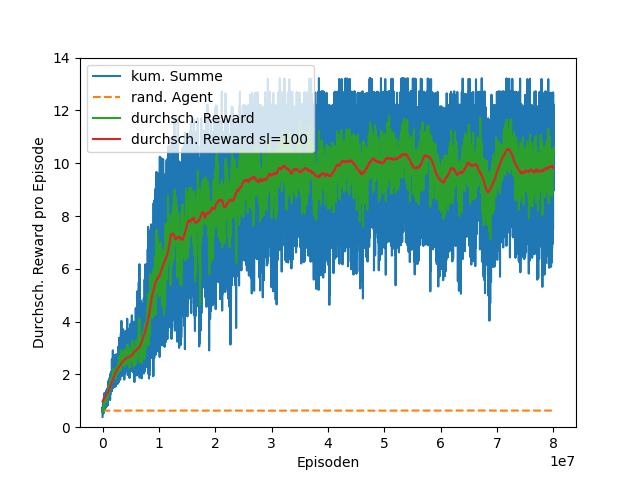
\includegraphics[scale=0.49]{abb/_graphen/floor_80Mio_200lvl_15act_Training}
        \caption{Blau: kumulierter Reward; Grün: durchschnittlicher kumulierter Reward; Rot: Grün mit SW 100; Orange: rand. Agent.}
        \label{fig:grph_floor_80Mio_200lvl_15act_Training}
    \end{minipage}
    \centering
    \begin{minipage}{0.48\linewidth}
        %\centering
        \textbf{Evaluation}\par\medskip
        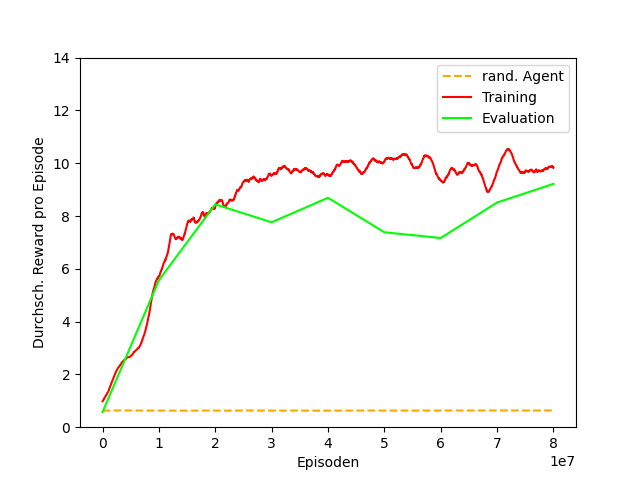
\includegraphics[scale=0.5]{abb/_graphen/floor_80Mio_200lvl_15act_Training_evalAsTraining}
        \caption{Evaluation: one-shot, 50 Level, 8 Checkpoints des Trainings.}
        \label{fig:grph_floor_80Mio_200lvl_15act_evalAsTraining}
        \hfil
    \end{minipage}
\end{figure}

\begin{center}
 \begin{table}[htb!]
 \begin{center}
  \begin{tabular}{ l c c c c }
    \hline
		      & Zeitschritte & Anzahl Level & Hintergrund & Farbe Orb \\ \hline \hline
     Training     & 80 Mio       & 200		 & 	    normal & r:0, g:255, b:0 \\ \hline
     Evaluation & - 	           & 50		 & 	    normal & r:0, g:255, b:0 \\ \hline
    \hline
  \end{tabular}
  \caption{Übersicht über geltende Rahmenbedingungen in Training und Evaluation - 1.}
  \label{tab:tab_durch_EXP_trainSetting1}
  \end{center}
 \end{table}
\end{center} 

Tabelle \ref{tab:tab_durch_EXP_trainSetting1} zeigt die geltenden Rahmenbedingungen während des Trainings. Die linke Abbildung (\ref{fig:grph_floor_80Mio_200lvl_15act_Training}) zeigt eine detaillierte Übersicht über das Training des Agenten. In blau wird der kumulierte Reward angegeben. Der grüne Graph gibt den durchschnittlichen kumulierten Reward an und der rote Graph zeigt den durchschnittlichen kumulierten Reward mit einem SW von 100. Die rechte Abbildung (\ref{fig:grph_floor_80Mio_200lvl_15act_evalAsTraining}) zeigt eine Evaluation von acht Checkpoints über den Verlauf des Trainings. Gemessen wird die one-shot Performance des Agenten in 50 ungesehenen Leveln pro Checkpoint. Jeder Checkpoint wird in denselben 50 Leveln evaluiert. Die Evaluation findet, abgesehen von den ungesehenen Leveln, unter Trainingsbedingungen statt. 

\begin{figure}[htb!]
    \begin{minipage}{\linewidth}
        \centering
        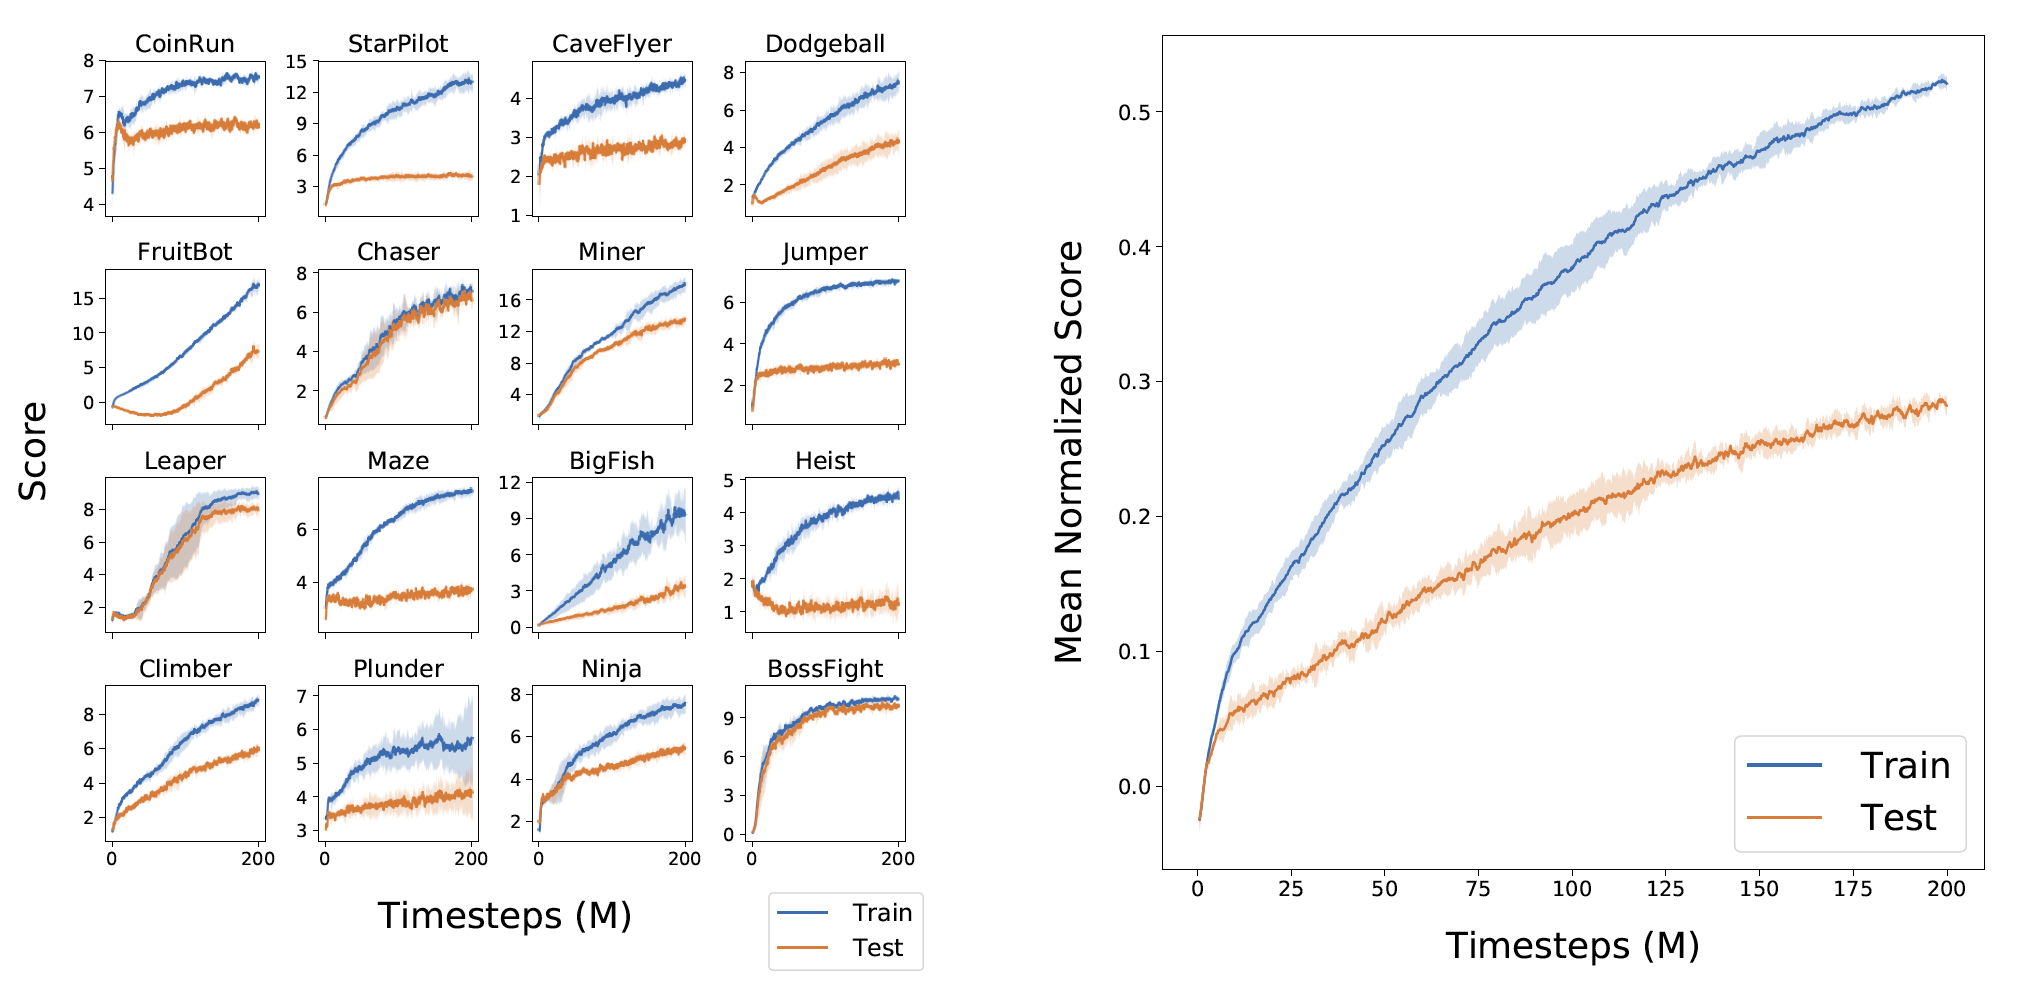
\includegraphics[scale=0.4]{abb/_graphen/procgen_fig4}
        \caption{Experiment zur Generalisierung des Procgen-Papers für 200 Mio. Zeitschritte, in 500 Leveln \cite{cobbe2019procgen}.}
        \label{generalization_500lvl_procgen}
    \end{minipage}
\end{figure}



\textbf{Diskussion:} Ein Vergleich zwischen der Abbildung \ref{fig:grph_floor_80Mio_200lvl_15act_evalAsTraining} und der Abbildung \ref{generalization_500lvl_procgen} zeigt, dass die Ergebnisse nicht nur reproduzierbar sind, sondern mit den eingesetzten Mitteln sogar übertroffen werden können. Im Paper von Procgen endet der Trainingsgraph von Chaser nach 500 Leveln, bei 200 Mio. Zeitschritten, bei einem Reward von etwa $7,2$ (vgl. \ref{generalization_500lvl_procgen}). Beim Reproduktions-Experiment wird nach 200 Leveln bei 80 Mio. Zeitschritten, ein Reward von etwa $9,8$ erreicht. Eine mögliche Erklärung für diese Diskrepanz ist die fehlende Angabe zum eingesetzten Skalierungsfaktor der IMPALA-Architektur für dieses Experiment. Der Vergleich der Ergebnisse in Abbildung \ref{fig:grph_floor_80Mio_200lvl_15act_evalAsTraining} mit der Abbildung \ref{generalization_500lvl_procgen} suggeriert jedoch, dass die Autoren an dieser Stelle eventuell einen kleineren Skalierungsfaktor, bspw. 2 statt 4, für die Architektur verwenden. Eine weitere mögliche Erklärung für die niedrigere Performance im Procgen-Paper könnte sein, dass über mehrere Seeds hinweg evaluiert wird und dass die Seeds der Autoren schwieriger sind, als der Seed, welcher in dieser Arbeit verwendet wird. Hierzu bietet die Arbeit \cite{cobbe2019procgen} jedoch ebenso keinen Hinweis. Die Abbildung Chaser im Procgen-Paper (\ref{generalization_500lvl_procgen}) zeigt auf, dass nahezu keine Generalisierungslücke zwischen Training und Evaluation besteht. Das bedeutet, dass der Agent über den Verlauf dieses Trainings generalisieren kann. Dieser Fakt kann ebenfalls reproduziert werden. Abbildung \ref{fig:grph_floor_80Mio_200lvl_15act_evalAsTraining} zeigt, dass wie im Paper fast keine Generalisierungslücke besteht. Der Leistungseinbruch bei den Checkpoints 50 Mio. und 60 Mio. ist im Rahmen der erwarteten Varianz von DRL. 

\paragraph{Antwort: Set 1, Punkt 1}
Somit kann in $\frac{2}{5}$ der Zeit und Level-Anzahl eine zufriedenstellende Reproduktion realisiert werden. Die erste Frage aus Set 1, kann also mit \dq Ja\dq{} beantwortet werden. Dadurch ist die Grundlage geschaffen, um weitere Experimente mit den eingesetzten Implementierungen durchzuführen. 


\subsubsection{Untersuchung zum Beitrag von prozeduraler Generierung bei DRL}\label{subsec:absch_EXP_durch_reproduktion_generalisierung}
\paragraph{Vergleich Level-Anzahl: 200, 1}\label{par:durch_EXP_vgl_200_1}
Der folgende Paragraph vergleicht zwei Agenten, welche sich einzig in der Anzahl der im Training verwendeten Levels unterscheiden.
Abbildung \ref{fig:grph_floor_80Mio_200lvl_15act_evalAsTraining_1} zeigt Training und Evaluation des Agenten, welcher mit einer fixen Anzahl von 200 Leveln trainiert ist. Dies ist derselbe Agent, wie in Abbildung \ref{fig:grph_floor_80Mio_200lvl_15act_Training}. Auf der rechten Seite ist ein weiterer Agent gezeigt. Der neue Agent ist unter denselben Umständen wie der Agent auf der linken Seite trainiert, mit dem Unterschied, dass der rechte Agent auf ein einziges Level im Training beschränkt ist.
\begin{figure}[htp!]
   \centering
   \captionsetup{width=0.45\linewidth} 
    \begin{minipage}{0.48\linewidth}
        \centering\
        \textbf{Level-Anzahl: 200}\par\medskip
        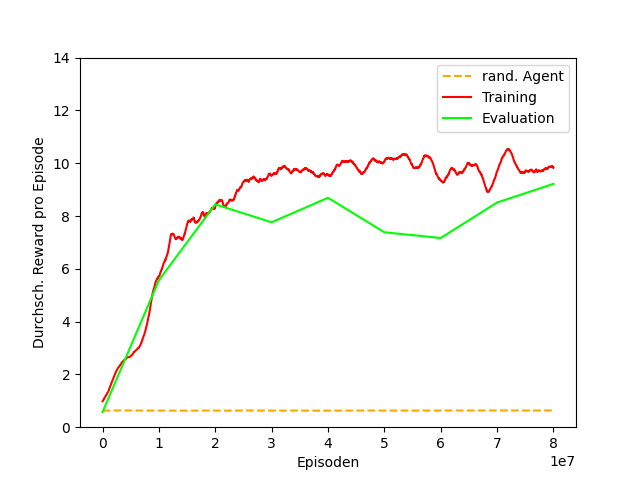
\includegraphics[scale=0.5]{abb/_graphen/floor_80Mio_200lvl_15act_Training_evalAsTraining}
        \caption{Evaluation: one-shot, Training mit fixer Level-Anzahl.}
        \label{fig:grph_floor_80Mio_200lvl_15act_evalAsTraining_1}
    \end{minipage}
    \centering
    \begin{minipage}{0.48\linewidth}
        \centering
        \textbf{Level-Anzahl: 1}\par\medskip
        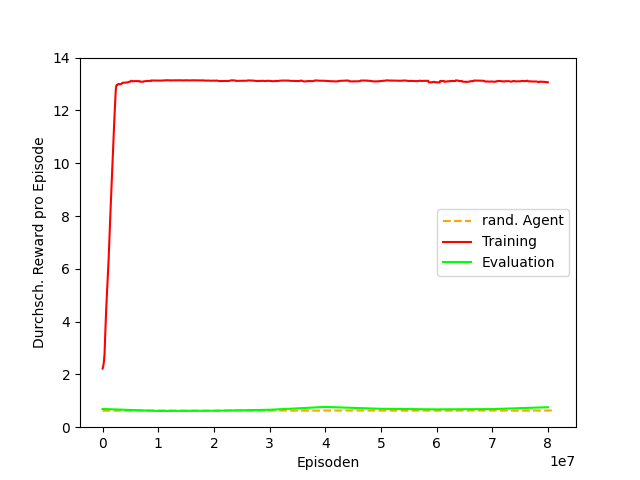
\includegraphics[scale=0.5]{abb/_graphen/floor_80Mio_1lvl_15act_Training_evalAsTraining}
        \caption{Evaluation: one-shot, Training mit unbeschr. Level-Anzahl.}
        \label{fig:grph_floor_80Mio_1lvl_15act_evalAsTraining}
    \end{minipage}
\end{figure}

\begin{center}
 \begin{table}[htb!]
 \begin{center}
  \begin{tabular}{ l c c c c }
    \hline
			       	& Zeitschritte 	& Anzahl Level 	& Hintergrund 	& Farbe Orb \\ \hline \hline
     Level-Anzahl 200 	& 80 Mio       	& 200		& 	    normal 	& r:0, g:255, b:0 \\ \hline
     Level-Anzahl 1     	& 80 Mio       	& 1			& 	    normal 	& r:0, g:255, b:0 \\ \hline
     Evaluation 		& - 	           	& 50			& 	    normal 	& r:0, g:255, b:0 \\ \hline
    \hline
  \end{tabular}
  \caption{Übersicht über geltende Rahmenbedingungen in Training und Evaluation - 2.}
  \label{tab:tab_durch_EXP_trainSetting2}
  \end{center}
 \end{table}
\end{center} 

\textbf{Diskussion:} Es ist eindeutig ersichtlich, dass der Agent, der nur auf einem Level trainiert wurde, im Training weitaus stabiler ist und allgemein mit einem höheren durchschnittlichen Reward pro Episode (hier in rot) abschneidet. Das bestätigt die Annahme des Papers von Zhan, Vinyal, Munos und Bengio \cite{zhang2018study}, dass ein RL-Agent mit Leichtigkeit auf ein kleines Trainings-Set overfitted. Die Evaluation der beiden Agenten (hier jeweils in grün) zeigt jedoch ebenso klar, dass der Agent, welcher nur auf einem Level trainiert, keinerlei Generalisierung aufweisen kann. Der Agent mit 200 Trainings-Leveln hingegen weist bereits fast keine Generalisierungslücke mehr auf. 

Um die zweite Frage des ersten Sets \ref{lst:itemList_EXP_durch_fragen1} vollständig beantworten zu können, ist ein weiteres Experiment notwendig, welches im folgenden Paragraphen erläutert wird. 


\paragraph{Vergleich Level-Anzahl: 200, unbeschränkt}\label{par:durch_EXP_vgl_200_unbeschr}
In diesem Paragraphen wird der Agent, welcher mit 200 Leveln trainiert wurde, mit einem weiteren Agenten verglichen. Procgen bietet die Möglichkeit im Training verschiedene Bedingungen für die Level-Auswahl des Trainings festzulegen. Unter anderem bietet die Umgebung die Möglichkeit eine unbeschränkte Level-Anzahl zu setzen. Somit wird im Training nach positivem oder negativem Abschluss einer Episode immer ein neues, unbekanntes Level bereitgestellt. Durch diese Umsetzung soll die prozedurale Eigenschaft der Level-Erstellung maximal ausgeschöpft werden.

Der neue Agent ist ebenfalls nahezu unter denselben Umständen trainiert, wie der Agent von Abbildung \ref{fig:grph_floor_80Mio_200lvl_15act_evalAsTraining_1}. Dieses Mal besteht der oben beschriebene Umstand, dass die Level-Anzahl im Training unbeschränkt ist. In Abbildung \ref{fig:grph_floor_80Mio_200lvl_15act_Training_1} befindet sich wieder der Agent mit beschränkter Level-Anzahl und Abbildung \ref{fig:grph_floor_80Mio_inflvl_15act_evalAsTraining} zeigt den neue Agenten mit unbeschränkter Level-Anzahl. 
\begin{figure}[htp!]
   \centering
   \captionsetup{width=0.45\linewidth} 
    \begin{minipage}{0.48\linewidth}
        \centering\
        \textbf{Level-Anzahl: 200}\par\medskip
        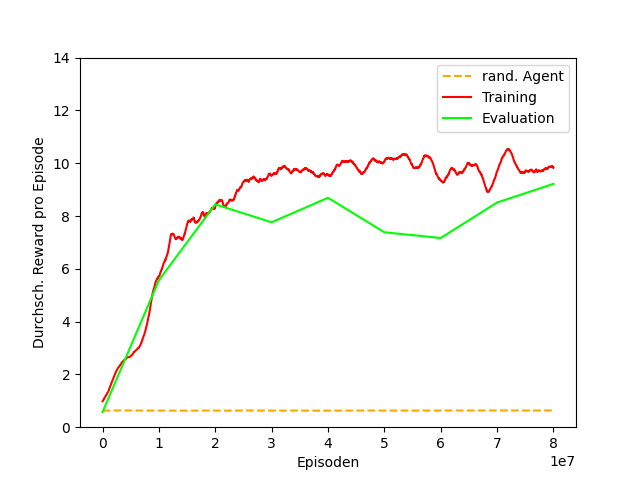
\includegraphics[scale=0.5]{abb/_graphen/floor_80Mio_200lvl_15act_Training_evalAsTraining}
        \caption{Evaluation: one-shot, auf 50 Leveln, 8 Checkpoints des Trainings}
        \label{fig:grph_floor_80Mio_200lvl_15act_Training_1}
    \end{minipage}
    \centering
    \begin{minipage}{0.48\linewidth}
        \centering
        \textbf{Unbeschränkt Level}\par\medskip
        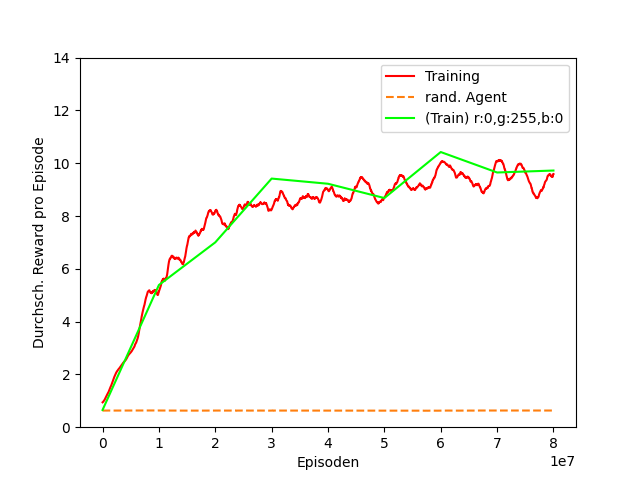
\includegraphics[scale=0.5]{abb/_graphen/floor_80Mio_inflvl_15act_Training_evalAsTraining_14}
        \caption{Evaluation: one-shot, auf 50 Leveln, 8 Checkpoints des Trainings}
        \label{fig:grph_floor_80Mio_inflvl_15act_evalAsTraining}
    \end{minipage}
\end{figure}

\begin{center}
 \begin{table}[htb!]
 \begin{center}
  \begin{tabular}{ l c c c c }
    \hline
		               & Zeitschritte & Anzahl Level & Hintergrund & Farbe Orb \\ \hline \hline
     200 Level           & 80 Mio       & 200		  & 	    normal & r:0, g:255, b:0 \\ \hline
     Unbeschr. Level & 80 Mio       & unbeschr.      & 	    normal & r:0, g:255, b:0 \\ \hline
     Evaluation 		& -	        	   & 1			  & 	    normal 	& r:0, g:255, b:0 \\ \hline
    \hline
  \end{tabular}
  \caption{Übersicht über geltende Rahmenbedingungen in Training und Evaluation - 3.}
  \label{tab:tab_durch_EXP_trainSetting3}
  \end{center}
 \end{table}
\end{center} 

\textbf{Diskussion:} Der direkte Vergleich der beiden Agenten zeigt eindeutig, dass die hohe intrinsische Diversität der Level-Distribution von Procgen \cite{cobbe2019procgen}[S.2] eine große Hilfe beim Erlernen von Generalisierung ist. Die Sample Efficiency ist von der prozeduralen Level-Generierung in diesem Fall weder positiv noch negativ beeinflusst. Das Procgen-Paper zeigt in seinem Experiment \emph{500 Level Generalization} jedoch klar, dass die Auswirkungen der Eigenschaften von Procgen nicht in allen Atari-Environments so drastisch sind (vgl. siehe Abbildung \ref{generalization_500lvl_procgen}). 

Das Spiel Chaser ist durch die Anwesenheit der Orbs eine einfache Umgebung für einen RL-Agenten, welcher auf optischen Inputs beruht. Die Orbs bieten dem Agenten dadurch, dass sie eingesammelt werden können die visuelle Information darüber, wo er schon gewesen ist und wo er noch hin muss. Darüber hinaus geben die Orbs beim einsammeln einen kleinen Reward. Auch wenn der Reward sehr klein ist (0,04 im Vergleich mit 10, implizit für den letzten Orb) leidet dieses Environment nicht unter dem bekannten \emph{Sparse-Reward-Problem}. 

Bei diesem Problem bietet das Environment des Agenten über lange Zeit keinen Reward und er ist darauf angewiesen viele Aktionen auszuführen, bevor überhaupt ein positiver Reward erwartet werden kann. Das Atari-Spiel \dq Montezuma's Revenge\dq{} stellt hierfür ein gutes Beispiel dar. Hier muss der Spieler häufig Schlüssel einsammeln, die zwar den Score erhöhen, jedoch gehören diese Schlüssel oft zu Türen, die mehrere Räume entfernt sein können.

\paragraph{Antwort: Set 1, Punkt 2}
Die zweite Frage des ersten Sets (\ref{lst:itemList_EXP_durch_fragen1}) kann nun vollständig beantwortet werden. Die aus der prozeduralen Level-Generierung resultierende unbeschränkte Anzahl an möglichen Trainings-Leveln bzw. Größe der Trainings-Sets, hilft im Chaser-Environment eindeutig die Generalisierungslücke zu schließen. Jedoch muss das Ergebnis weiter mit größeren Experimenten untersucht werden, bspw. über mehrere Seeds hinweg. Das hier durchgeführte Experiment unterstützt lediglich die Hypothese, dass die intrinsische Diversität ideal für die Evaluation von Generalisierung und Sample Efficiency ist \cite{cobbe2019procgen}[S.9]. 


%################################################################################################################
%################################################################################################################
%FARBÄNDERUNGEN
%################################################################################################################
%##################################################################################################   ##############
\subsection{Visuelle Augmentation - Farbänderungen}\label{absch_EXP_durch_serie1}
Im folgenden Unterkapitel werden Experimente durchgeführt, welche visuelle Änderungen des Trainings- bzw. Evaluations-Environments untersuchen. Die Änderungen des Environments werden in den jeweiligen Experimenten dargelegt.

\subsubsection{Maskierung der Orbs}\label{sub_absch_EXP_durch_serie1_orbsMaskieren}
Wie in Unterkapitel \ref{absch_RL_chaser} erwähnt, ist es das Ziel des Agenten in Chaser alle Orbs einzusammeln. Erst dann gilt eine Episode als erfolgreich abgeschlossen. Dadurch eignen sich die Orbs für Maskierungen und Änderungen ihre Anwesenheit bzw. Erscheinung. Zu diesem Zweck wird im Environment das Hintergrundbild durch eines derselben Größe mit der RGB-Farbe (r:0, g:255, b:0) monoton ersetzt. Die gewählte Farbe entspricht der Farbe der Orbs und maskiert ihre visuelle Anwesenheit. Ein Bild des resultierenden Inputs für den Agenten kann dem Anhang  \ref{anh_env_bilder_chaser} der Abbildung \emph{Hintergrund grün} entnommen werden. Dem Agenten fehlt damit jede visuelle Information der Orbs. Das Reward-System bleibt weiter bestehen. Betritt der Agent ein Feld, welches er zuvor noch nicht besucht hat, bekommt er den Orb-Reward von 0,04. Das aufgeführte Experiment zeigt das Training und die Evaluation eines Agenten, welcher für 5 Mio. Zeitschritte auf einem Level trainiert. Dieses Experiment weicht von der one-shot Evaluation, wie in \ref{subsec_EXP_durch_fragen} definiert ab. Hier ist jeder Checkpoint 50 Mal auf dem einen bekannten Trainings-Level evaluiert.



\begin{figure}[htp!]
   \centering
   \captionsetup{width=0.45\linewidth} 
    \begin{minipage}{0.48\linewidth}
        \centering\
        \textbf{Training - 5 Mio. Zeitschritte}\par\medskip
        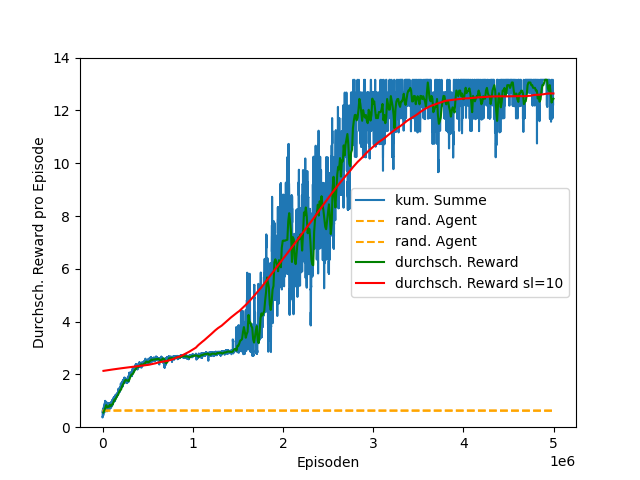
\includegraphics[scale=0.5]{abb/_graphen/green_5Mio_1lvl_15act_Training}
        \caption{Training mit monoton grünem Hintergrund.}
        \label{fig:grph_green_5Mio_1lvl_15act_Training}
    \end{minipage}
    \centering
    \begin{minipage}{0.48\linewidth}
        \centering
        \textbf{Evaluation}\par\medskip
        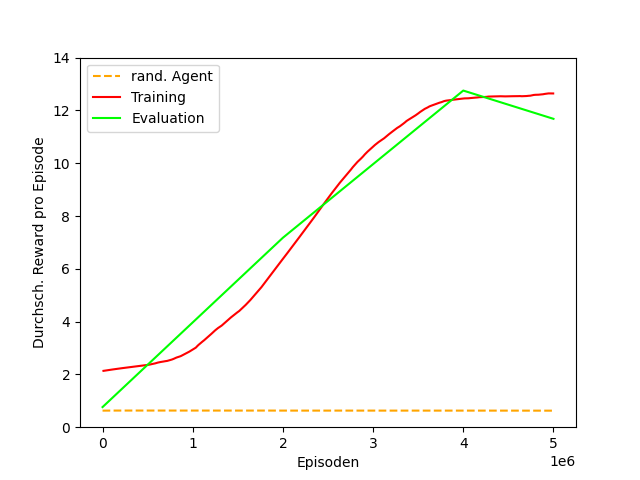
\includegraphics[scale=0.5]{abb/_graphen/green_5Mio_1lvl_15act_Training_evalAsTraining} 
        \caption{Eval: one-shot, auf bekanntem Level.}
        \label{fig:grph_green_5Mio_1lvl_15act_Training_evalAsTraining}
    \end{minipage}
\end{figure}

\begin{center}
%\vskip-0.5cm
 \begin{table}[htb!]
 \begin{center}
  \begin{tabular}{ l c c c c }
    \hline
			       	& Zeitschritte 	& Anzahl Level 	& Hintergrund 	& Farbe Orb \\ \hline \hline
     Level-Anzahl 1     	& 5 Mio       	& 1			& 	     r:0, g:255, g:0	& r:0, g:255, b:0 \\ \hline
     Evaluation 		& - 	           	& 1			& 	    r:0, g:255, g:0 	& r:0, g:255, b:0 \\ \hline
    \hline
  \end{tabular}
  \caption{Übersicht über geltende Rahmenbedingungen in Training und Evaluation - 4.}
  \label{tab:tab_durch_EXP_trainSetting4}
  \end{center}
 \end{table}
\end{center} 

\textbf{Diskussion:} Trotz des grünen Hintergrunds, welcher die visuellen Orb-Informationen maskiert, ist der Agent bereits nach 2,8 Mio. Zeitschritten in der Lage das Level im Training konsistent zu lösen. Auf die Evaluation in ungesehenen Leveln kann hier vorerst verzichtet werden, da in Unterkapitel \ref{par:durch_EXP_vgl_200_1} schon gezeigt wird, dass ein Agent mit einem einzelnen Trainings-Level nicht generalisiert. 
Der Graph von Abbildung \ref{fig:grph_green_5Mio_1lvl_15act_Training_evalAsTraining} zeigt starkes Overfitting auf dem Trainings-Level. Wie dieses Trainingsszenario mit maskierter Orb-Information in größerem Maßstab abläuft, wird im folgenden Paragraphen untersucht.

\paragraph{Vergleich Level-Anzahl: 200, unbeschr., mit grünem Hintergrund}\label{par:durch_EXP_vgl_200_unbeschr_green}
Für das folgende Experiment werden zwei Agenten, einer mit 200 Trainings-Leveln und einer mit unbeschränkter Level-Anzahl, für 80 Mio. Zeitschritte trainiert. Bei diesen Trainings ist der Hintergrund, wie im Paragraphen zuvor, monoton in derselben Farbe wie die Orbs und maskiert deren visuelle Erscheinung. Hierfür werden zwei neue Agenten trainiert.

\begin{figure}[htp!]
   \centering
   \captionsetup{width=0.45\linewidth} 
    \begin{minipage}{0.48\linewidth}
        \centering\
        \textbf{200 Level}\par\medskip
        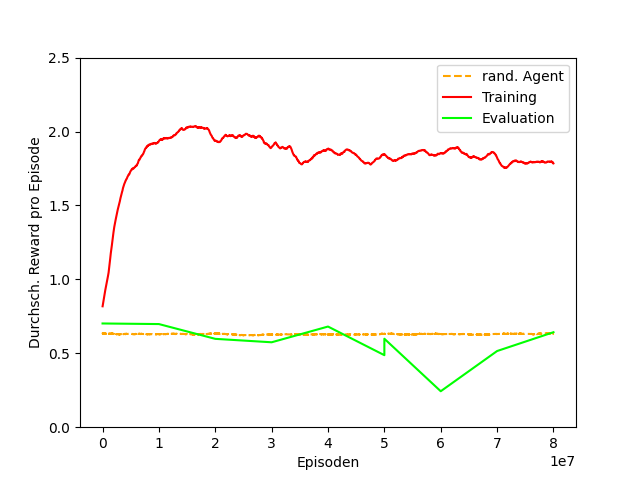
\includegraphics[scale=0.5]{abb/_graphen/green_80Mio_200lvl_15act_Training_evalAsTraining}
        \caption{Training mit grünem Hintergrund in 200 Leveln}
        \label{fig:grph_green_80Mio_200lvl_15act_Training_evalAsTraining_}
    \end{minipage}
    \centering
    \begin{minipage}{0.48\linewidth}
        \centering
        \textbf{Unbeschränkt Level}\par\medskip
        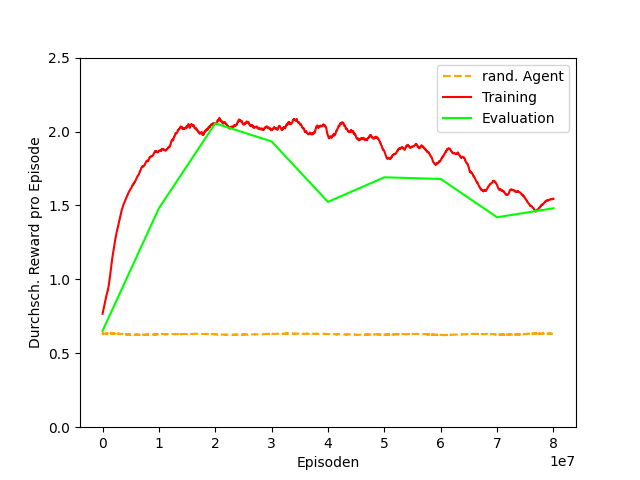
\includegraphics[scale=0.5]{abb/_graphen/green_80Mio_inflvl_15act_Training_evalAsTraining} 
        \caption{Training mit grünem Hintergrund in unbeschr. Leveln}
        \label{fig:grph_green_80Mio_inflvl_15act_Training_evalAsTraining_}
    \end{minipage}
\end{figure}

\begin{center}
%\vskip-0.5cm
 \begin{table}[htb!]
 \begin{center}
  \begin{tabular}{ l c c c c }
    \hline
			       	& Zeitschritte 	& Anzahl Level 	& Hintergrund	 	& Farbe Orb \\ \hline \hline
     200 Level     	& 80 Mio       	& 200		&  r:0, g:255, g:0	& r:0, g:255, b:0 \\ \hline
     Unbeschr. Level   	& 80 Mio       	& unbeschr.	&  r:0, g:255, g:0	& r:0, g:255, b:0 \\ \hline
     Evaluation 		& - 	           	& 50			&  r:0, g:255, g:0 	& r:0, g:255, b:0 \\ \hline
    \hline
  \end{tabular}
  \caption{Übersicht über geltende Rahmenbedingungen in Training und Evaluation - 5.}
  \label{tab:tab_durch_EXP_trainSetting5}
  \end{center}
 \end{table}
\end{center} 

Abbildung \ref{fig:grph_green_80Mio_200lvl_15act_Training_evalAsTraining_} zeigt den Agenten, welcher für 80 Mio. Zeitschritte auf 200 verschiedenen Leveln trainiert wurde. Abbildung \ref{fig:grph_green_80Mio_inflvl_15act_Training_evalAsTraining_} zeigt den Agenten, welcher ebenfalls für 80 Mio. Zeitschritte trainiert wurde, jedoch mit unbeschränkter Level-Anzahl. 

\textbf{Diskussion:} Der Agent mit 200 Leveln im Training zeigt keinerlei Generalisierung. Bei 60 Mio. Zeitschritten lernt der Agent sogar etwas, was ihn schlechter als den zufällig laufenden Agenten macht. Im Kontrast dazu schließt der Agent, welcher mit einer unbeschränkten Level-Anzahl trainiert wurde, die Generalisierungslücke. Vergleicht man hingegen diese beiden Agenten mit den Agenten, welche die Orb-Information während des Trainings haben (\ref{par:durch_EXP_vgl_200_unbeschr}), kristallisiert sich die Hypothese heraus, dass die Orbs eine notwendige visuelle Information darstellen. Beide Agenten mit grünem Hintergrund, egal in wie vielen Leveln sie trainiert wurden, erreichen keine konstanten Siege im Environment. Genauer zeigt die Evaluation, dass keiner der Agenten auch nur ein Level erfolgreich abgeschlossen hat. Diese Ergebnisse werfen die Frage auf, wie ein Agent abschneidet, welcher mit der visuellen Orb-Information trainiert ist, wenn ihm in der Evaluation diese Information entzogen wird. \\


\begin{figure}[htp!]
   \centering
   \captionsetup{width=0.45\linewidth} 
    \begin{minipage}{0.48\linewidth}
        \centering\
        \textbf{Fehlende Orb-Information}\par\medskip
        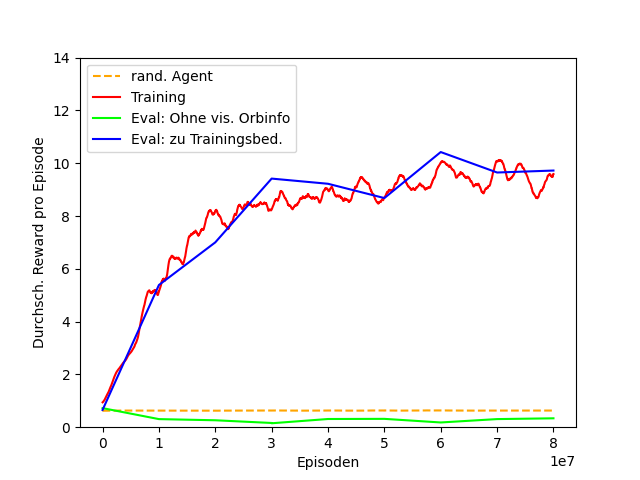
\includegraphics[scale=0.5]{abb/_graphen/floor_80Mio_inflvl_15act_Training_evalAsTraining_evalNoOrb}
        \caption{Evaluation mit und ohne visuelle Orb-Information.}
        \label{fig:floor_80Mio_inflvl_15act_Training_evalAsTraining_evalNoOrb}
    \end{minipage}
\end{figure}

\begin{center}
%\vskip-0.5cm
 \begin{table}[htp!]
 \begin{center}
  \begin{tabular}{ l c c c c }
    \hline
		               & Zeitschritte & Anzahl Level & Hintergrund & Farbe Orb \\ \hline \hline
     Training              & 80 Mio       & unbeschr.	  & 	    normal & r:0, g:255, b:0 \\ \hline
     Eval. wie Training & -              & 50	           & 	    normal & r:0, g:255, b:0 \\ \hline
     Eval. ohne Orbs 	& -	        	   & 50		  & 	    normal 	& vis. nicht vorhanden \\ \hline
    \hline
  \end{tabular}
  \caption{Übersicht über geltende Rahmenbedingungen in Training und Evaluation - 6.}
  \label{tab:tab_durch_EXP_trainSetting6}
  \end{center}
 \end{table}
\end{center} 


%\subsubsection{}

Um die Hypothese zu bestätigen, wird der Agent aus Experiment \ref{par:durch_EXP_vgl_200_unbeschr} mit unbeschränkten Trainings-Leveln wiederverwendet. Dieser Agent weist die beste Generalisierung der bisher trainierten Agenten auf und eignet sich daher am besten für dieses Experiment. Abbildung \ref{fig:floor_80Mio_inflvl_15act_Training_evalAsTraining_evalNoOrb} zeigt die Evaluation mit und ohne visuelle Information der Orbs. Die Agenten sind beide auf denselben Leveln evaluiert. 

\textbf{Diskussion:} Die beiden Graphen zeigen eindeutig, dass die visuelle Information der Orbs unentbehrlich für den Erfolg im gewählten Spiel sind. Beim Start des Trainings zeigt der Agent ohne die visuelle Information (hier grün) noch dieselbe Performance wie der Random-Agent (hier orange-gestrichelt). Bereits beim ersten Checkpoint nach 10 Mio. Zeitschritten im Training, ist seine Performance schlechter als die des Random-Agenten. Die Leistung der anderen Checkpoints oszilliert um einen Wert unterhalb dem des Random-Agenten. 

\paragraph{Antwort: Set 2, Punkt 1}
Nun kann die erste Frage des zweiten Sets (\ref{lst:itemList_EXP_durch_fragen2}) beantwortet werden. Die visuelle Information der Orbs ist notwendig, um unbekannte Level erfolgreich abzuschließen. Es ist egal, ob ein Agent mit dieser Restriktion schon im Training oder erst in der Evaluation konfrontiert wird. Die allgemeine Performance reicht kaum über die eines Random-Agentrn hinaus. Weiter zeigt Abbildung \ref{fig:grph_green_80Mio_inflvl_15act_Training_evalAsTraining_}, dass die Performance der Agenten ab ca. 20 Mio. Zeitschritten sowohl im Trainings, als auch in der Evaluation einen Abwärtstrend aufweist. 


\subsubsection{Farbänderungen der Orbs}\label{sub_absch_EXP_durch_farbÄnderungen}
Im vergangenen Unterkapitel wird gezeigt, dass die visuelle Information der Orbs  ein essenzieller Bestandteil zum erfolgreichen Abschluss unbekannter Level ist. Im folgenden Unterkapitel wird untersucht, welche Auswirkungen farbliche Änderungen der Orbs in der Evaluation auf die Performance eines Agenten haben, der keine dieser Änderungen im Training gesehen hat. Weiter wird hier untersucht, ob eine Konzeptualisierung des Orbs im Training stattfindet. Hierfür wird zunächst wieder der Agent aus Paragraph \ref{par:durch_EXP_vgl_200_unbeschr_green}, mit unbeschränkter Level-Anzahl und normalem Hintergrund, weiteren Evaluationen unterzogen. 


\paragraph{Zufälliger Wert für Grün}\label{par:durch_EXP_farbÄnd_grünZufällig}
Zuerst wird untersucht, wie die Performance in der Evaluation ausfällt, wenn dem Orb in jedem Frame ein neuer Wert für g in RGB, mitgegeben wird. Ein Frame dieser Einstellung kann dem Anhang \ref{anh_env_bilder_chaser} dem Bild \emph{Orb-Farbe: gruen, zufaellig 0-255} entnommen werden. Resultierend aus der Änderung der Orb-Farbe in jedem Frame, flackert jeder Orb in verschiedenen Grüntönen.

\begin{figure}[htp!]
   \centering
   \captionsetup{width=0.45\linewidth} 
    \begin{minipage}{0.48\linewidth}
        \centering\
        \textbf{Zufällige Grüntöne}\par\medskip
        \includegraphics[scale=0.5]{abb/_graphen/floor_80Mio_inflvl_15act_Training_evalRandomGreens}
        \caption{Evaluation mit zufälligen Grüntönen der Orbs}
        \label{fig:floor_80Mio_inflvl_15act_Training_evalRandomGreens}
    \end{minipage}
\end{figure}

\begin{center}
%\vskip-0.5cm
 \begin{table}[htp!]
 \begin{center}
  \begin{tabular}{ l c c c c }
    \hline
		               & Zeitschritte & Anzahl Level & Hintergrund & Farbe Orb \\ \hline \hline
     Training              & 80 Mio       & unbeschr.	  & 	    normal & r:0, g:255, b:0 \\ \hline
     Eval. zufälliges Grün 	& -	        	   & 50		  & 	    normal 	& r:0, g:0-255, b:0 \\ \hline
     Eval. zufälliges Grün 	& -	        	   & 50		  & 	    normal 	& r:0, g:1-255, b:0 \\ \hline
    \hline
  \end{tabular}
  \caption{Übersicht über geltende Rahmenbedingungen in Training und Evaluation - 7.}
  \label{tab:tab_durch_EXP_trainSetting7}
  \end{center}
 \end{table}
\end{center} 

Der blaue Graph zeigt die Evaluation mit einem zufälligen Grünton, ohne die Option auf schwarze Orbs - der rote Graph zeigt die Evaluation mit der Option auf schwarze Orbs. 

\textbf{Diskussion:} Die Auswertung dieser Daten legt vorerst nahe, dass keine Konzeptualisierung des Orbs stattfindet und dennoch ist der Agent bei den Checkpoints ab 60 Mio. Zeitschritte deutlich besser, als der Random-Agent. Hier muss erwähnt werden, dass die Zuweisung einer neuen, zufälligen Orb-Farbe in jedem Frame eine starke Änderung der gewohnten Pixel-Verteilung darstellt. So zeigt der Agent in beiden Evaluationen keine befriedigende Generalisierung für diese Änderungen auf. Motiviert durch dieses Experiment wird im folgenden Paragraphen untersucht, wie sich eine statische Änderung des Grün-Anteils auf die Performance auswirkt.

\paragraph{Grünabstufungen in 50er Schritten}\label{par:durch_EXP_farbÄnd_grünAbstufung}
Zur Erinnerung, die Farbe der Orbs im Training hat die RGB-Werte (r:0, g:255, b:0). Hier wird in jeder Evaluation der grün-Wert (G-Wert) um 50 verringert, angefangen bei 250 bis 0. Die Graphen der Abbildung, außer dem Trainingsgraphen, haben alle die jeweilige Farbe, die in der Evaluation verwendet wurde.

\begin{figure}[htp!]
   \centering
   \captionsetup{width=0.45\linewidth} 
    \begin{minipage}{0.48\linewidth}
        \centering\
        \textbf{50er Grüntöne - 1}\par\medskip
        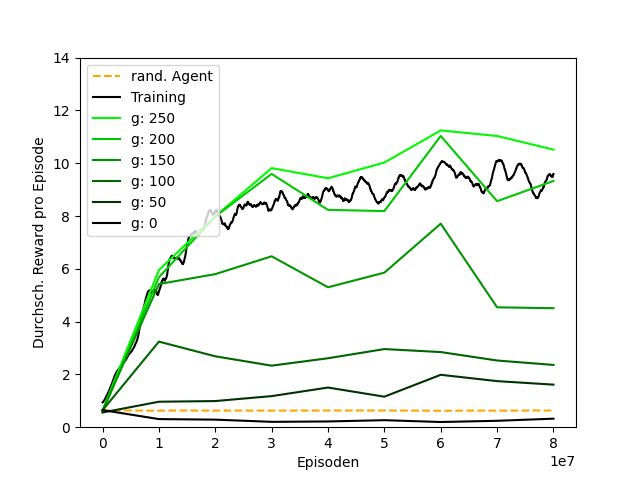
\includegraphics[scale=0.5]{abb/_graphen/floor_80mio_inflvl_Training_eval50Green}
        \caption{Evaluation von Grüntönen, schwärzer werdend.}
        \label{fig:floor_80Mio_inflvl_15act_Training_eval50Green}
    \end{minipage}
\end{figure}
\begin{center}
 \begin{table}[htp!]
 \begin{center}
  \begin{tabular}{ l c c c c }
    \hline
		               & Zeitschritte & Anzahl Level & Hintergrund & Farbe Orb \\ \hline \hline
     Training              & 80 Mio       & unbeschr.	  & 	    normal & r:0, g:255, b:0 \\ \hline
     Eval. Grün: 250 	& -	        	   & 50		  & 	    normal 	& r:0, g:250, b:0 \\ \hline
     Eval. Grün: 200 	& -	        	   & 50		  & 	    normal 	& r:0, g:200, b:0 \\ \hline
     Eval. Grün: 150 	& -	        	   & 50		  & 	    normal 	& r:0, g:150, b:0 \\ \hline
     Eval. Grün: 100 	& -	        	   & 50		  & 	    normal 	& r:0, g:100, b:0 \\ \hline
     Eval. Grün: 50 	& -	        	   & 50		  & 	    normal 	& r:0, g:50, b:0 \\ \hline
     Eval. Grün: 0 	& -	        	   & 50		  & 	    normal 	& r:0, g:0, b:0 \\ \hline
    \hline
  \end{tabular}
  \caption{Übersicht über geltende Rahmenbedingungen in Training und Evaluation - 8.}
  \label{tab:tab_durch_EXP_trainSetting8}
  \end{center}
 \end{table}
\end{center} 

\textbf{Diskussion:} Die Auswertung der Abbildung \ref{fig:floor_80Mio_inflvl_15act_Training_eval50Green} zeigt eine interessante These. Die Ergebnisse zeigen, dass die Performance stetig abnimmt, solange der G-Wert weiter abnimmt. Mit jeder weiteren Evaluation wird die Generalisierungslücke größer. So weisen die beiden Graphen mit einem G-Wert von $200$ und $250$ fast gleich gute Performance und nahezu keine Probleme bei der Generalisierung auf. Wohingegen der Graph mit einem G-Wert von $150$ kaum besser als halb so gut ist, wie die zwei Graphen zuvor. Die restlichen drei Graphen mit den G-Werten $100$, $50$ und $0$ zeigen einen stetigen Abstieg der Performance in der Evaluation. Bei einem G-Wert von 0 ist der Agent sogar schlechter als der Random-Agent.

Um die These weiter zu untersuchen, wird folgend ein ähnliches Experiment vorgestellt, in dem der G-Wert konstant bei $255$ ist und sich die Werte für rot und blau von Evaluation zu Evaluation verändern. Zuvor wurden die Orbs dunkler und dunkler, bis hin zu schwarz - folgend werden die Orbs immer heller, bis hin zu weiß. Wie zuvor haben die Graphen der Abbildung \ref{fig:floor_80Mio_inflvl_15act_Training_eval50Others} die Orb-Farbe der jeweiligen Evaluation. Die Farbe Weiß wird hier aus Gründen der Sichtbarkeit in Grau dargestellt.  \newline

\begin{figure}[htp!]
   \centering
   \captionsetup{width=0.45\linewidth} 
    \begin{minipage}{0.48\linewidth}
        \centering\
        \textbf{50er Grüntöne - 2}\par\medskip
        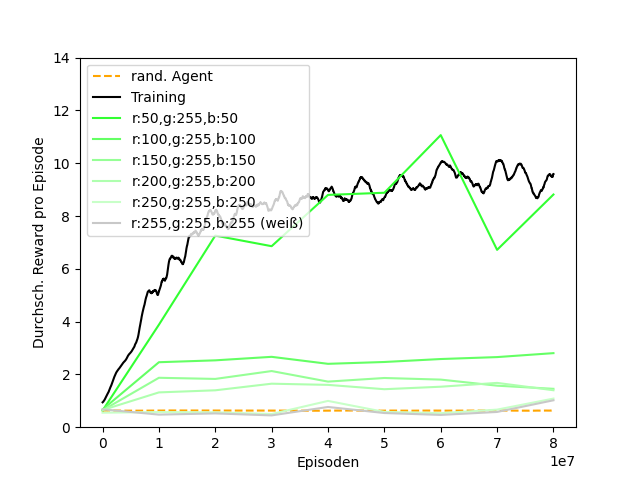
\includegraphics[scale=0.5]{abb/_graphen/floor_80mio_inflvl_Training_eval50Others}
        \caption{Evaluation von Grüntönen, weißer werdend.}
        \label{fig:floor_80Mio_inflvl_15act_Training_eval50Others}
    \end{minipage}
\end{figure}
\begin{center}
 \begin{table}[htp!]
 \begin{center}
  \begin{tabular}{ l c c c c }
    \hline
		               			& Zeitschritte & Anzahl Level & 		Hintergrund & Farbe Orb \\ \hline \hline
     Training              			& 80 Mio       & unbeschr.	  & 	    		normal & r:0, g:255, b:0 \\ \hline
     Eval. r:50, b:50	 	& -	        	   & 50		  	  &			normal & r:50, g:255, b:50 \\ \hline
     Eval. r:100, b:100	& -	        	   & 50		  & 	    				normal & r:100, g:255, b:100  \\ \hline
     Eval. r:150, b:150 	& -	        	   & 50		  & 	    			normal & r:150, g:255, b:150  \\ \hline
     Eval. r:200, b:200 	& -	        	   & 50		  & 	    			normal & r:200, g:255, b:200 \\ \hline
     Eval. r:250, b:250 	& -	        	   & 50		  & 	    			normal & r:250, g:255, b:250 \\ \hline
     Eval. r:255, b:255 	& -	        	   & 50		  & 	    			normal & r:255, g:255, b:255 \\ \hline
    \hline   
  \end{tabular}
  \caption{Übersicht über geltende Rahmenbedingungen in Training und Evaluation - 9.}
  \label{tab:tab_durch_EXP_trainSetting9}
  \end{center}
 \end{table}
\end{center} 

\textbf{Diskussion:} Die Auswertung der Abbildung \ref{fig:floor_80Mio_inflvl_15act_Training_eval50Others} liefert Ergebnisse, welche die zuvor aufgestellte These vorerst widerlegen. Verglichen mit Abbildung \ref{fig:floor_80Mio_inflvl_15act_Training_eval50Green} zeigt Abbildung \ref{fig:floor_80Mio_inflvl_15act_Training_eval50Others} keinen stetigen Abstieg der Performance mit fortlaufender Evaluation. Stattdessen schneiden die Evaluationen mit R- und B-Werten $100$ bis $255$ deutlich schlechter ab, als die Evaluation mit schwärzer werdenden Orbs. Darüber hinaus zeigen die Graphen mit den R- und B-Werten (R-Werte, B-Werte) $100$ bis $250$ eine deutlich geringere Varianz, als die korrespondierenden Graphen der Abbildung \ref{fig:floor_80Mio_inflvl_15act_Training_eval50Green}. Eine mögliche Erklärung für die generell schlechtere Leistung der Graphen mit R- und B-Werten von $100$ bis $250$ kann sein, dass die Abweichung der Orb-Farbe, verglichen zur Farbe im Training, an zwei Farbwerten der RGB-Farbe verändert wurde. Dementgegen wurde in der Evaluation von Abbildung \ref{fig:floor_80Mio_inflvl_15act_Training_eval50Green} jeweils nur der G-Wert verändert. 

Die Veränderung an zwei Stellschrauben der RGB-Farbe stellt im Kontext des gesamten Bildes eine größere Veränderung der Pixel-Verteilung dar. Aus beiden Experimenten dieses Paragraphen geht hervor, dass jene Durchläufe, bei denen die Abweichung der farblichen Distanz zu einem Input-Frame vom Training zu stark sind, generell schlecht abscheiden. So stellt eine Veränderung der Orbs um jeweils 50 in den R- und B-Werten (100 gesamt) keine Herausforderung für den Agenten aus Abbildung \ref{fig:floor_80Mio_inflvl_15act_Training_eval50Others} dar. Dagegen hat eine Änderung um 105 am G-Wert, verglichen mit dem Trainingszustand des Orbs, deutlich gravierendere Auswirkungen auf die Performance (siehe Abbildung \ref{fig:floor_80Mio_inflvl_15act_Training_eval50Green}).  
Das bestätigt die intuitive These, dass Änderungen an zwei der drei Pixel-Werte und die daraus resultierende Änderung der Pixel-Verteilung größere Auswirkungen auf die Performance hat, als Änderungen an nur einem der Werte. Weiter lässt sich aus den Ergebnissen schließen, dass der Agent stark auf die Farbe des Orbs overfitted. Diese These wird im folgenden Paragraphen genauer untersucht. 


\paragraph{Experimente mit verschiedenen Orb-Farben}
\label{par:durch_EXP_farbÄnd_rgbOrbfarben}

Für die folgenden Experimente werden zwei weitere Agenten trainiert. Einer mit roten und einer mit blauen Orbs (\emph{Agent-Rot} und \emph{Agent-Blau}), beide mit dem normalen Hintergrund. Bilder des jeweiligen Inputs der Agenten können dem Anhang entnommen werden (\ref{anh_env_bilder_chaser}, Titel: \emph{Blaue Orbs}, \emph{Rote Orbs}). Beide neuen Agenten sind für eine Dauer von 80 Mio. Zeitschritten und mit einer unbeschränkten Anzahl an Leveln trainiert. Die Agenten unterscheiden sich somit lediglich in der Farbe, welche die Orbs während des Trainings haben. 

In dieser Reihe von Experimenten werden die oben beschrieben Agenten, mit dem in Unterkapitel \ref{sec:absch_EXP_durch_reproduktion} vorgestellten Agenten mit normalem Hintergrund und grünen Orbs (\emph{Agent-Grün}) verglichen. Dieser Agent dient hier als Baseline für den Vergleich der Agenten. In der Evaluation wird jeder Agent zum Vergleich mit seiner Orb-Farbe wie im Training und den Trainingsfarben der beiden anderen Agenten konfrontiert. Alle Agenten haben den jeweiligen Farb-Channel auf 255 und die anderen beiden auf 0 gesetzt. So entspricht die Farbe Rot dem RGB-Wert $ r:255, g=0, b=0 $, die anderen Farben ergeben sich analog. Somit weisen die drei Orb-Farben eine farbliche Distanz von $510$ auf.

\begin{figure}[htp!]
   \centering
   \captionsetup{width=0.48\linewidth} 
    \begin{minipage}{0.48\linewidth}
        \centering\
        %\medskip
        \textbf{Training - Rot}\par
        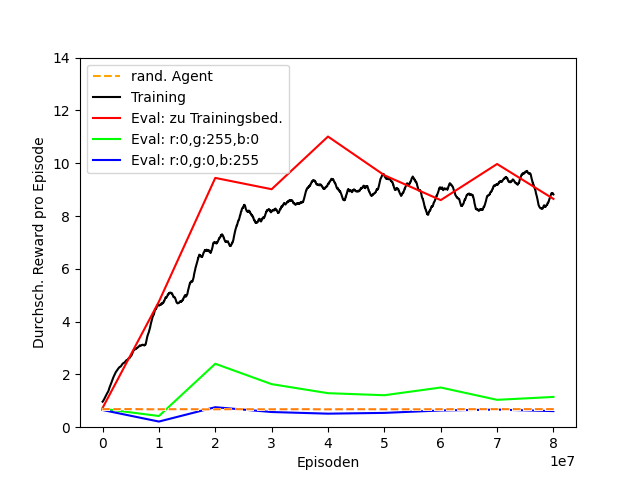
\includegraphics[scale=.358]{abb/_graphen/floor_80Mio_inflvl_15_act_TrainingRot_evalRGB}
        \caption{Training mit rotem Orb und normalem Hintergrund.}
        \label{fig:grph_red_80Mio_200lvl_15act_Training_evalAsTraining}
    \end{minipage}
    \centering
    \begin{minipage}{0.48\linewidth}
        \centering
        \textbf{Training - Grün}\par%\medskip 
        %0,49
        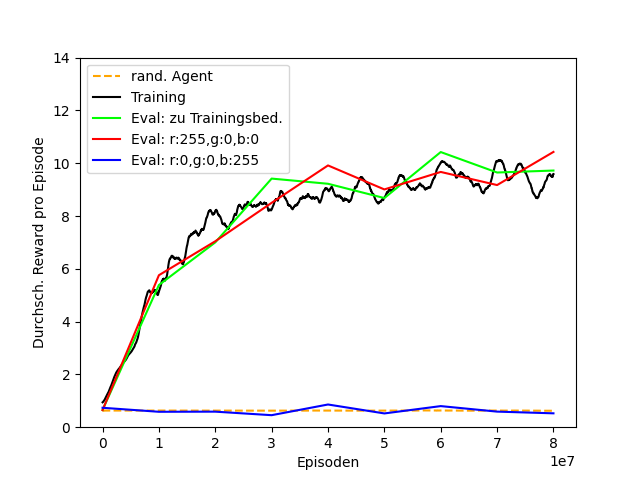
\includegraphics[scale=0.515]{abb/_graphen/floor_80Mio_inflvl_15_act_TrainingGreen_evalRGB} 
        \caption{Training mit grünem Orb und normalem Hintergrund.}
        \label{fig:grph_green_80Mio_inflvl_15act_Training_evalAsTraining}
    \end{minipage}
    \centering
    \begin{minipage}{0.48\linewidth}
    	\centering
        \textbf{Training - Blau}\par%\medskip
        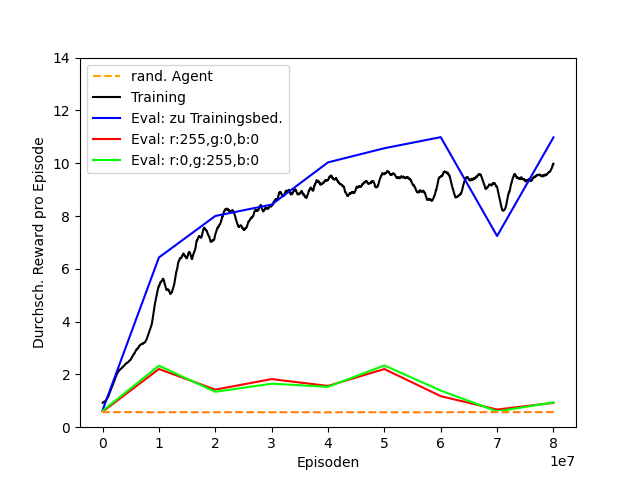
\includegraphics[scale=0.358]{abb/_graphen/floor_80Mio_inflvl_15_act_TrainingBlau_evalRGB} 
        \caption{Training mit blauem Orb und normalem Hintergrund.}
        \label{fig:grph_blue_80Mio_inflvl_15act_Training_evalAsTraining}
    \end{minipage}
\end{figure}

\begin{center}
 \begin{table}[htp!]
 \begin{center}
  \begin{tabular}{ l c c c c }
    \hline
		               			& Zeitschritte & Anzahl Level & 		Hintergrund & Farbe Orb \\ \hline \hline
     Training rot              			& 80 Mio       & unbeschr.	  & 	    		normal & r:255, g:0, b:0 \\ \hline
     Training grün              			& 80 Mio       & unbeschr.	  & 	    		normal & r:0, g:255, b:0 \\ \hline
     Training blau             			& 80 Mio       & unbeschr.	  & 	    		normal & r:0, g:0, b:255 \\ \hline
     Eval. rot	 	& -	        	   & 50		  	  &			normal & r:255, g:0, b:50 \\ \hline
     Eval. grün	& -	        	   & 50		  & 	    				normal & r:0, g:255, b:0  \\ \hline
     Eval. blau 	& -	        	   & 50		  & 	    			normal & r:0, g:0, b:255  \\ \hline
    \hline
  \end{tabular}
  \caption{Übersicht über geltende Rahmenbedingungen in Training und Evaluation - 10.}
  \label{tab:tab_durch_EXP_trainSetting10}
  \end{center}
 \end{table}
\end{center} 

\textbf{Diskussion:} Im Training zeigen die unterschiedlichen Agenten sehr ähnliche Leistungen. Keiner der trainierten Agent weist eine relevante Generalisierungslücke auf. Die Abweichungen von der Baseline Agent-Grün ist im Rahmen der erwarteten Varianz, bei der Verwendung tiefer NNs. Wie zu erwarten, ist eine Änderung der Orb-Farbe während der Evaluation eine unüberwindbare Hürde für die Agenten. Dies gilt jedoch nicht für den Agent-Grün. Dieser Agent ist in der Lage mit der unbekannten Orb-Farbe Rot, eine nahezu identische Performance während der Evaluation zu erreichen. Die Evaluationen mit unbekannten Orb-Farben der Agenten Agent-Rot und Agent-Blau ist zwar weit unter der Performance der Evaluation zu Trainingsbedingungen, dennoch sind die beiden Agenten in drei von vier Fällen besser, als der Random-Agent. In Abbildung \ref{fig:grph_red_80Mio_200lvl_15act_Training_evalAsTraining} (Agent-Rot) weist der Graph, welcher die Evaluation mit einem grünen Orb zeigt, eine deutliche Abweichung vom Random-Agenten auf. Die Abweichung wird in Abbildung \ref{fig:grph_blue_80Mio_inflvl_15act_Training_evalAsTraining} noch deutlicher. Hier ist der Agent-Blau in der Lage, mit beiden unbekannten Orb-Farben (hier rot und grün) eine noch deutlichere Abweichung zum Random-Agenten aufzuweisen. Genauer performt der Agent-Blau mit beiden unbekannten Farben nahezu gleich gut. Der Einsturz der Leistung beim Checkpoint 70 Mio. Zeitschritte spiegelt sich ebenso in der Evaluation mit der bekannten Orb-Farbe wieder und ist über ein schlechtes Update der Policy zu erklären. 

In diesem Experiment werden zwar die Orb-Farben in die drei Extreme verändert (siehe Tabelle \ref{tab:tab_durch_EXP_trainSetting10}), jedoch ist der Hintergrund weiterhin ein farbiges Bild mit Textur (siehe Abbildung \ref{fig:pic_chaserGros}). Da die jeweiligen Farben der Orbs einen Farbkanal auf $255$ und die anderen beiden auf $0$ haben, stellen diese Farben die Grundfarbtöne von RBG dar. Um eine der drei Farben weiß zu machen, müssen die beiden Farbkanäle, welche auf $0$ sind, ebenfalls auf $255$ gesetzt werden. Somit weisen alle drei Orb-Farben eine farbliche Distanz zur Farbe Weiß von $510$ RGB-Werten auf.

Um die Unterschiede in der farblichen Distanz der jeweiligen Orb-Farben zum Hintergrund auszuschließen, wird das hier aufgeführte Experiment mit einem weißen Hintergrund wiederholt. 


\paragraph{Experimente mit weißem Hintergrund}\label{par:durch_EXP_farbÄnd_weisserHintergrund}

Im folgenden Paragraphen wird das Experiment der vorangegangenen Paragraphen mit einem weißen Hintergrund wiederholt. Dies soll Unterschiede der jeweiligen Orb-Farbe zum Hintergrund bezüglich Kontrast ausschließen und stellt sicher, dass die Farben alle die selbe farbliche Distanz zum Hintergrund haben. Hierfür werden drei neue Agenten, mit der eben erwähnten Veränderung zu den selben Bedingungen, wie im vorherigen Experiment trainiert. 

Wie zuvor bezeichnet \emph{Agent-Rot} den Agenten welcher mit einem roten Orb trainiert wird. \emph{Agent-Grün} bezeichnet den Agenten mit grünen und \emph{Agent-Blau} den mit blauen Orbs im Training. Ein Bild des aktuellen Agenten-Inputs kann dem Anhang den Bildern mit dem Titel \emph{BG: weiß} entnommen werden (\ref{anh_env_bilder_chaser}).

\begin{figure}[htp!]
   \centering
   \captionsetup{width=0.48\linewidth} 
    \begin{minipage}{0.48\linewidth}
        \centering\
        %\medskip
        \textbf{Training - Rot}\par
        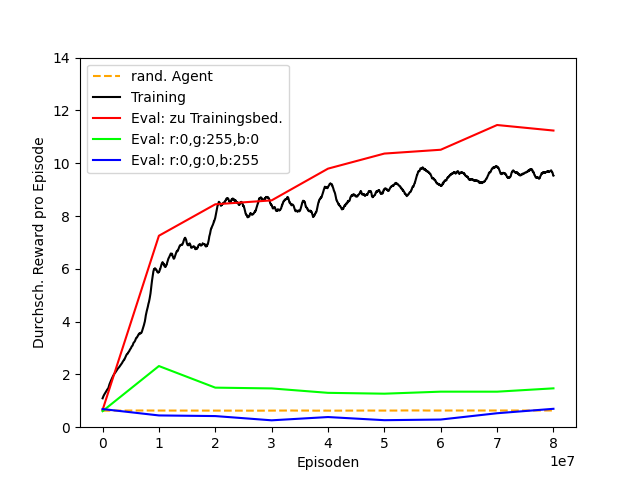
\includegraphics[scale=.5]{abb/_graphen/floor_80Mio_inflvl_15_act_TrainingRot_evalRGB_white}
        \caption{Training mit rotem Orb und weißem Hintergrund.}
        \label{fig:grph_red_80Mio_200lvl_15act_Training_evalAsTraining_white}
    \end{minipage}
    \centering
    \begin{minipage}{0.48\linewidth}
        \centering
        \textbf{Training - Grün}\par%\medskip 
        %0,49
        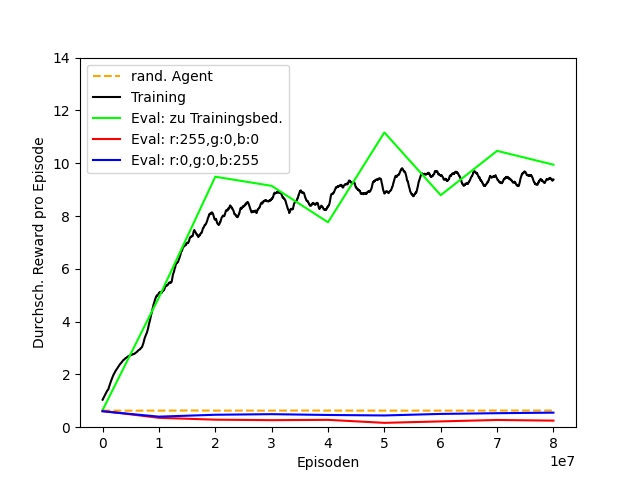
\includegraphics[scale=0.5]{abb/_graphen/floor_80Mio_inflvl_15_act_TrainingGreen_evalRGB_white} 
        \caption{Training mit grünem Orb und weißem Hintergrund.}
        \label{fig:grph_green_80Mio_inflvl_15act_Training_evalAsTraining_white}
    \end{minipage}
    \centering
    \begin{minipage}{0.48\linewidth}
\vspace*{0.5cm}
    	\centering
        \textbf{Training - Blau}\par%\medskip
        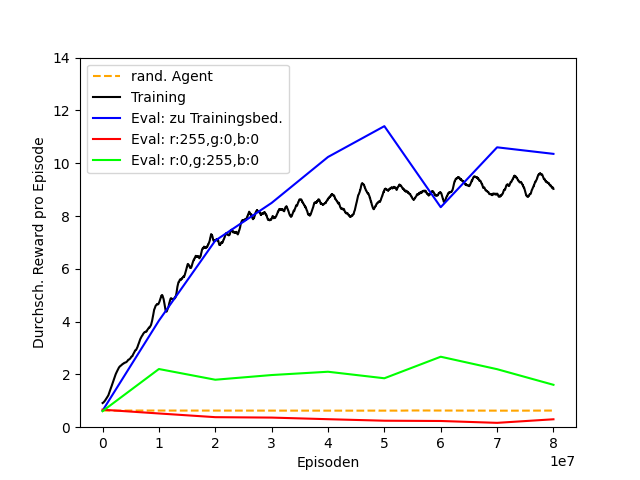
\includegraphics[scale=0.5]{abb/_graphen/floor_80Mio_inflvl_15_act_TrainingBlau_evalRGB_white} 
        \caption{Training mit blauem Orb und weißem Hintergrund.}
        \label{fig:grph_blue_80Mio_inflvl_15act_Training_evalAsTraining_white}
    \end{minipage}
\end{figure}
\begin{center}
 \begin{table}[htp!]
 \begin{center}
  \begin{tabular}{ l c c c c }
    \hline
		               			& Zeitschritte & Anzahl Level & 		Hintergrund & Farbe Orb \\ \hline \hline
     Training rot              			& 80 Mio       & unbeschr.	  & 	    		weiß & r:255, g:0, b:0 \\ \hline
     Training grün              			& 80 Mio       & unbeschr.	  & 	    		weiß & r:0, g:255, b:0 \\ \hline
     Training blau             			& 80 Mio       & unbeschr.	  & 	    		weiß & r:0, g:0, b:255 \\ \hline
     Eval. rot	 	& -	        	   & 50		  	  &			weiß & r:255, g:0, b:50 \\ \hline
     Eval. grün	& -	        	   & 50		  & 	    				weiß & r:0, g:255, b:0  \\ \hline
     Eval. blau 	& -	        	   & 50		  & 	    			weiß & r:0, g:0, b:255  \\ \hline
    \hline
  \end{tabular}
  \caption{Übersicht über geltende Rahmenbedingungen in Training und Evaluation - 11.}
  \label{tab:tab_durch_EXP_trainSetting10}
  \end{center}
 \end{table}
\end{center} 


\textbf{Diskussion:} Wie im oben aufgeführten Experiment, zeigen die Abbildungen \ref{fig:grph_red_80Mio_200lvl_15act_Training_evalAsTraining_white}, \ref{fig:grph_green_80Mio_inflvl_15act_Training_evalAsTraining_white} und \ref{fig:grph_blue_80Mio_inflvl_15act_Training_evalAsTraining_white}, dass die Evaluationen zu Trainingsbedingungen nahezu keine Generalisierungslücke aufweist. Weiter ist Agent-Grün nicht mehr in der Lage, mit den roten Orbs genauso hohe Rewards, wie mit den bekannten grünen Orbs zu erzielen, wie im Experiment zuvor. Hier ist sogar das Gegenteil der Fall. Der Graph der Evaluation mit rotem Orb (\ref{fig:grph_green_80Mio_inflvl_15act_Training_evalAsTraining_white}) ist über jeden Checkpoint hinweg unter dem des Random-Agenten und auch unter dem Graphen der Evaluation mit blauem Orb. Darüber hinaus sind nicht mehr drei von vier Graphen (unterschiedlicher Farben) der Agenten aus den Abbildungen \ref{fig:grph_red_80Mio_200lvl_15act_Training_evalAsTraining_white} und \ref{fig:grph_blue_80Mio_inflvl_15act_Training_evalAsTraining_white} besser als der Random-Agent. Lediglich die Graphen der jeweiligen Evaluation mit grünen Orbs sind besser als der Random-Agent. \\

\paragraph{Antwort: Set 2, Punkt 2}
Die zwei Fragen des zweiten Punkts vom Set zur farblichen Änderung (\ref{par_EXP_durch_fragen2}) sind mit den durchgeführten Experimenten nicht mit ausreichender Sicherheit zu beantworten. Die erste Frage kann klar beantwortet werden. Über das Training mit den geltenden Bedingungen findet keine Konzeptualisierung eines Orbs bezogen auf farbliche Änderungen statt. Die vier Experimente in Unterkapitel \ref{sub_absch_EXP_durch_farbÄnderungen} belegen empirisch, dass jede Veränderung der visuellen Darstellung des Orbs drastische Auswirkungen auf den erhaltenen Reward des Agenten haben. 

Die zweite Frage kann zwar  beantwortet werden, jedoch widersprechen die Ergebnisse der initialen Intuition und werfen wiederum selbst neue Fragen auf. Die beschriebenen Experimente bestätigen, dass sich farbliche Änderungen, nahezu jeder farblichen Distanz, negativ auswirken. Allerdings kann der Agent sein Wissen in diesem einen Fall abstrahieren. So ist der Agent aus Abbildung \ref{fig:grph_green_80Mio_inflvl_15act_Training_evalAsTraining} in der Lage, mit der unbekannten Orb-Farbe Rot, nahezu identische Rewards zu erzielen, wie in der Evaluation zu Trainingsbedingungen mit grünem Orb. Ein blauer Orb hingegen, welcher dieselbe farbliche Distanz zu einem grünen Orb hat, bricht die Generalisierung des Agenten in ungesehenen Leveln. 



\subsubsection{Untersuchung des Speichervermögens}

\paragraph{Experiment zum Speichervermögen}\label{par:durch_EXP_farbÄnd_Speichervermögen}
Folgend wird untersucht, wie viele Level ein Agent innerhalb einer begrenzten Anzahl an Zeitschritten auswendig lernen kann. Das Experiment im Anhang \ref{anh_exp_5mio} zeigt, dass ein Agent im Training bereits nach ca. 1,2 Mio. Zeitschritten in einem Level einen Reward von $ \geq 10$ erreicht. Somit overfitted der Agent bereits nach 1,2 Mio. Zeitschritten stark auf das Trainings-Level. Das Experiment mit grünem Hintergrund zu denselben Trainingsbedingungen zeigt, dass das Level nach circa 2,6 Mio. Zeitschritten ebenso problemlos bestanden werden kann, auch ohne die visuelle Information der Orbs. Diese Ergebnisse motivieren die folgenden Experimente.

Dieses Experiment untersucht mit 30 Agenten, wie viele Level ein Agent im Training innerhalb von 5 Mio. Zeitschritten auswendig lernen kann. Es wird nicht dieselbe one-shot Evaluation wie zuvor angewandt. Dieses Mal wird nach jeder Episode, eines der Trainings-Level, zufällig ausgewählt und das über 50 Iterationen hinweg. Die 30 Agenten sind in zwei Sets mit je 15 Agenten aufgeteilt. Das eine Set trainiert mit dem normalen und das andere mit dem grünem Hintergrund und somit mit maskierter, visueller Orb-Information. Der erste Agent eines Sets trainiert in einem Level, der zweite in zwei usw. Der letzte trainiert in 15 Leveln. Egal in wie vielen Leveln trainiert wird, dem Agenten stehen nur die 5 Mio. Zeitschritte zur Verfügung. Die ersten Balken von links der Abbildungen \ref{fig:grph_floor_80Mio_200lvl_15act_Training_evalAsTraining_1to15} und \ref{fig:grph_green_80Mio_inflvl_15act_Training_evalAsTraining_1to15} repräsentiert den ersten Agenten eines Sets, der Balken ganz rechts den letzten. Jeder Balken ist in vier Abschnitte unterteilt. Der unterste Teil zeigt den ersten Checkpoint (hier rot) nach dem ersten Zeitschritt und zeigt somit ebenso einen Random-Agenten. Checkpoint 2 (hier grün) den Agenten nach 2 Mio. Zeitschritten und Checkpoint 3 (hier blau) nach 4 Mio. Zeitschritten. Der letzte (hier cyan) zeigt die abschließende Evaluation nach 5 Mio. Zeitschritten. Der Anhang bietet eine tabellarische Übersicht über die Erfolgsraten der jeweiligen Agenten (\ref{anh_exp_erfolgsrate}). 

\begin{figure}[htp!]
   \centering
   \captionsetup{width=0.45\linewidth} 
    \begin{minipage}{0.48\linewidth}
        \centering\
        \textbf{Normaler Hintergrund\\0 bis 15 Level}\par\medskip
        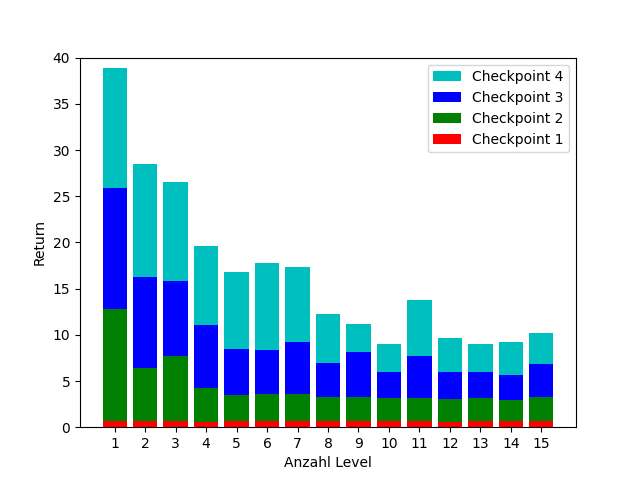
\includegraphics[scale=0.5]{abb/_graphen/serie_auswendig_floor}
        \caption{Training in 1 - 15 Leveln mit normalem Hintergrund.}
        \label{fig:grph_floor_80Mio_200lvl_15act_Training_evalAsTraining_1to15}
    \end{minipage}
    \centering
    \begin{minipage}{0.48\linewidth}
        \centering
        \textbf{Grüner Hintergrund\\0 bis 15 Level}\par\medskip
        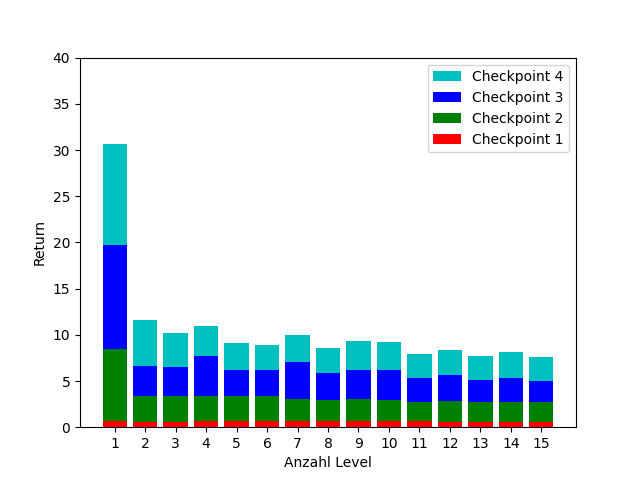
\includegraphics[scale=0.5]{abb/_graphen/serie_auswendig_green} 
        \caption{Training in 1 - 15 Leveln mit grünem Hintergrund.}
        \label{fig:grph_green_80Mio_inflvl_15act_Training_evalAsTraining_1to15}
    \end{minipage}
\end{figure}

\begin{center}
%\vskip-0.5cm
 \begin{table}[htb!]
 \begin{center}
  \begin{tabular}{ l c c c c }
    \hline
			       				& Zeitschritte 	& Anzahl Level 	& Hintergrund	 	& Farbe Orb \\ \hline \hline
     Train. normaler BG  	& 5 Mio       	& 1 - 15		&  normal			& r:0, g:255, b:0 \\ \hline
     Train. grüner BG   	& 5 Mio       	& 1 - 15 		&  r:0, g:255, g:0	& r:0, g:255, b:0 \\ \hline
     Eval. normaler BG 	& - 	           	& 1 - 15			&  normal		 	& r:0, g:255, b:0 \\ \hline
     Eval. grünem BG 	& - 	           	& 1 - 15			&  r:0, g:255, g:0 	& r:0, g:255, b:0 \\ \hline
    \hline
  \end{tabular}
  \caption{Übersicht über geltende Rahmenbedingungen in Training und Evaluation - 12.}
  \label{tab:tab_durch_EXP_trainSetting5}
  \end{center}
 \end{table}
\end{center} 

\textbf{Diskussion:} Der erste Agent von Abbildung \ref{fig:grph_floor_80Mio_200lvl_15act_Training_evalAsTraining_1to15} im direkten Vergleich mit dem ersten Agenten der Abbildung \ref{fig:grph_green_80Mio_inflvl_15act_Training_evalAsTraining_1to15} zeigt einerseits, dass die Performance der jeweiligen Checkpoints mit der visuellen Orb-Information höher ist, was auf eine bessere Sample Efficiency schließen lässt. Andererseits ist der gesamte erhaltene Reward jedes Checkpoints deutlich höher, als der des Agenten mit grünem Hintergrund. Die visuelle Anwesenheit der Orbs verhilft einem Agent also nicht nur zu verbesserter Sample Efficiency, sondern verhilft ihm auch zu einer robusteren Policy. Das lässt sich dadurch erklären, dass die Orbs, sofern sichtbar, eingesammelt werden können und nicht mehr vorhanden sind, sobald sie einmal eingesammelt sind. Das kann dem Agenten helfen eine zielführendere Strategie zu wählen. Das funktioniert jedoch nur unter der Prämisse, dass der Agent eine Vorstellung des finalen Ziels des Environments hat. Die Agenten zwei bis neun der linken Abbildung unterscheiden sich stark von denen der rechten. Die Agenten mit visueller Orb-Information sind in der Lage, bis zu drei Level innerhalb der 5 Mio. Zeitschritte auswendig zu lernen. Der Reward des vierten Checkpoints des dritten Agenten von Abbildung \ref{fig:grph_floor_80Mio_200lvl_15act_Training_evalAsTraining_1to15} liegt bei $10,71$. Dieser Agent schafft 76\% der 50 Wiederholungen seiner Trainings-Level. Im Vergleich hierzu schafft der vierte Checkpoint des ersten Agent aus Abbildung \ref{fig:grph_green_80Mio_inflvl_15act_Training_evalAsTraining_1to15} 78\% dieser Wiederholungen. Der dritte Agent derselben Abbildung schafft lediglich 8\% der Level. Der direkte Vergleich der dritten Agenten der beiden Abbildungen legt nahe, dass die visuelle Information der Orbs ein wichtiger Faktor für den erfolgreichen Abschluss unbekannter Level ist. Hier ergibt sich eine Differenz der Erfolgsrate von 68\%. Diese Ergebnisse unterstützen die des Experiments zur ersten Frage des zweiten Sets. Die Evaluation der letzten vier Agenten der beiden Sets legt nahe, dass die Performance des Agenten mit der visuellen Orb-Information weiter abnehmen wird, bis auf das Niveau der letzten Agenten aus Abbildung \ref{fig:grph_green_80Mio_inflvl_15act_Training_evalAsTraining_1to15}.\\

\paragraph{Antwort: Set 2, Punkt 3}
Nun können auch die zwei letzten Fragen des zweiten Sets beantwortet werden. Zuerst wird die erste Frage beantwortet. Innerhalb der beschränkten Anzahl an Zeitschritten im Training kann die verwendete Architektur 3 Level auswendig lernen. Der dritte Agent aus Abbildung \ref{fig:grph_floor_80Mio_200lvl_15act_Training_evalAsTraining_1to15} erreicht nach 5 Mio. Zeitschritten einen durchschnittlichen Reward von $10,71$. Nach der Definition einer bestandenen Evaluation in \ref{absch_RL_chaser} kann man sagen, dass der Agent die Evaluation mit drei Leveln besteht. Die Tabelle im Anhang (\ref{anh_exp_erfolgsrate}) zeigt, dass dieser Agent die Level zu 76\% erfolgreich besteht. 

Die zweite Frage ist eindeutig zu beantworten. Die Orbs bzw. ihre visuelle Existenz ist sehr relevant für einen erfolgreichen Abschluss der Evaluation. Dieses Experiment unterstützt damit die Hypothese des zweiten Experiments in \ref{sub_absch_EXP_durch_serie1_orbsMaskieren}, dass die kleinen Orbs eine notwendige visuelle Information darstellen. Wie am Anfang dieses Experiments erwähnt, zeigt Abbildung \ref{anh_exp_5mio} im Anhang, dass es circa 2,6 Mio. Zeitschritte benötigt, um ein Level ohne visuelle Orb-Information erfolgreich abzuschließen. Somit ist es nur logisch, dass innerhalb derselben Zeit keine zwei Level gelernt werden können. Dennoch ist die Beantwortung dieser Frage aufschlussreich. Der letzte Agent im Set mit normalem Hintergrund erreicht einen durchschnittlichen Reward, von $2,55$ über alle vier Checkpoints. Der letzte Agent des Sets mit grünem Hintergrund hat einen durchschnittlichen Reward der Checkpoints von $1,89$. Bei 15 Leveln ist der Unterschied der Performance beiden letzten Agenten der Sets nur noch bei $0,66$ ($2,55-1,89=0,66$). Die Agenten der Abbildung \ref{fig:grph_floor_80Mio_200lvl_15act_Training_evalAsTraining_1to15} zeigen alle den Trend, sich an den erhaltenen Reward der Agenten der Abbildung \ref{fig:grph_green_80Mio_inflvl_15act_Training_evalAsTraining_1to15} anzunähern. Jedoch zeigt sich auch, dass die Agenten mit visueller Orb-Information im Training über die 15 Evaluationen hinweg konstant besser sind als die Agenten, welche ohne diese Information trainiert sind. Ein Experiment mit einer größeren Anzahl an Zeitschritten und Leveln im Training könnte weiteren Aufschluss über visuelle Relevanz der Orbs geben.

%################################################################################################################
%################################################################################################################
%SEMANTISCHE INVERTIERUNG
%################################################################################################################
%################################################################################################################
\subsection{Visuelle Augmentation - Semantische Invertierung}\label{absch_EXP_durch_serie2}
Im folgenden Unterkapitel sind Experimente aufgeführt, welche sich mit visueller semantischer Invertierung beschäftigen. Das bedeutet, dass die Mechanik von optisch vertauschten Spielelementen weiterhin bestehen bleibt. Vertauscht man auf diese Weise die Semantik von bspw. der Mauer und den kleinen Orbs, kann der Agent nun, zumindest optisch, Mauern einsammeln und kleine Orbs bilden das Labyrinth. Somit sind alle Änderungen an Chaser in diesem Kapitel ausschließlich visueller Natur. Ein Bild des veränderten Environments kann dem Anhang entnommen werden (\ref{anh_env_bilder_chaser}, Titel: \emph{Default Spiel mit Orb-Sprite}). Im folgenden Kapitel wird wieder one-shot evaluiert, wie in \ref{subsec_EXP_durch_fragen} definiert. Das bedeutet, dass die beide Evaluationen auf denselben 50 Leveln stattfinden. Da die Orbs im Spiel Chaser als farbliche Quadrate ohne Textur implementiert sind, muss für dieses Experiment ein neuer Agent verwendet werden. Hierbei ist die Darstellung des Orbs durch ein Sprite ersetzt. Dies ermöglicht das Tauschen der beiden Sprites. 

\paragraph{Invertierung - Mauer und kleine Orbs}
Der folgenden Paragraph beschreibt Experimente, die sich mit der visuellen semantischen Invertierung der Mauer und der kleinen Orbs beschäftigen. Hierfür wird das optische Erscheinungsbild dieser beiden Spielelemente vertauscht. Der rote Graph der Abbildung \ref{fig:semChange_mauerklOrb_80Mio_15act_training_} zeigt die Evaluation zu Trainingsbedingungen, der schwarze zeigt das Training. In dunklem Blau ist die Evaluation mit vertauschter Semantik. Wie zuvor zeigt die orangene gestrichelte Linie den Random-Agenten. 
Ein Bild des Agenten-Inputs kann dem Anhang entnommen werden (\ref{anh_env_bilder_chaser}, Titel: \emph{Sprite-Tausch: kleiner Orb u.
Wand}). 

\begin{figure}[htp!]
   \centering
   \captionsetup{width=0.60\linewidth} 
    \begin{minipage}{0.48\linewidth}
        \centering\
        \textbf{Invertierung Mauer u. kleine Orbs}\par\medskip
        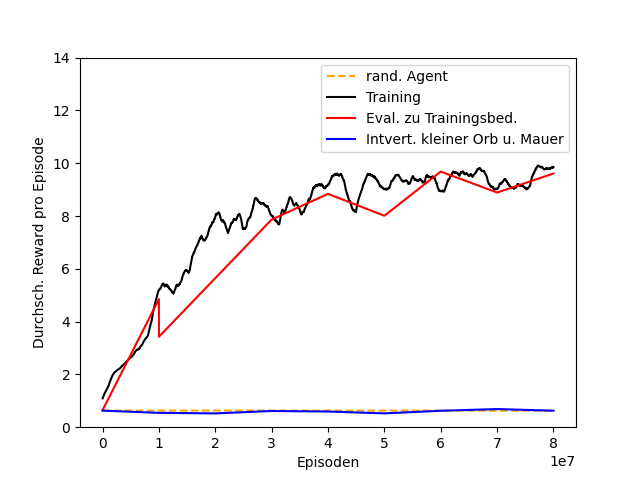
\includegraphics[scale=0.5]{abb/_graphen/semChange_mauerklOrb_80Mio_15act_training_}
        \caption{Evaluation zu Trainingsbed. und mit Invertierung der Mauer und kl. Orbs}
        \label{fig:semChange_mauerklOrb_80Mio_15act_training_}
    \end{minipage}
\end{figure}
\begin{center}
 \begin{table}[htp!]
 \begin{center}
  \begin{tabular}{ l c c c }
    \hline
		               			& Zeitschritte & Anzahl Level & 	 Invertierung\\ \hline
     Training              			& 80 Mio       & unbeschr.	    & 	 keine \\ \hline
     Eval. zu Trainingsbed.		& -	        	     & 50		    &	 keine \\ \hline
     Eval. Invertierung		 	& -	        	     & 50		    &	 Maucher u. kl. Orbs \\ \hline
    \hline
  \end{tabular}
  \caption{Übersicht über geltende Rahmenbedingungen in Training und Evaluation - 13.}
  \label{tab:tab_durch_EXP_trainSetting13}
  \end{center}
 \end{table}
\end{center} 

\textbf{Diskussion:} Die Evaluation zu Trainingsbedingungen (Abbildung \ref{fig:semChange_mauerklOrb_80Mio_15act_training_}) unterstützt die bisher gezeigten Ergebnisse. Ein Agent schafft es innerhalb von 80 Mio. Zeitschritten und einer unbeschränkten Level-Anzahl im Training die Generalisierungslücke zu schließen. Diese Evaluation bestätigt die Ergebnisse des Experiments in \ref{subsec:absch_EXP_durch_reproduktion_generalisierung}. Dagegen schafft der Graph der Evaluation mit semantischer Invertierung schafft es zu keinem Zeitpunkt über den des Random-Agenten hinaus. Eine mögliche Erklärung hierfür wäre, dass diese Änderung der Pixel-Verteilung zu stark ist. Im Verhältnis gibt es am Anfang eines Levels mehr kleine Orbs als Mauern. Vertauscht man nun diese beiden Sprites ist das Verhältnis umgedreht, wodurch sich die Pixel-Verteilung eines Frames stark verschiebt. Aufgrund dieser drastischen Änderung kann die Feature Extraction Pipeline die korrekten Features nicht mehr bereitstellen, um ein unbekanntes Level erfolgreich abzuschließen. Der folgende Paragraph beschreibt ein Experiment welches darauf aus ist, trotz semantischer Invertierung die Verschiebung der Pixel-Verteilung möglichst klein zu belassen.

\paragraph{Antwort: Set 3, Punkt 1}
Die Antwort auf diese Frage ist klar. Der Agent ist zu keinem Zeitpunkt besser als der Random-Agent. Somit ist die visuelle semantische Invertierung der Sprites des kleinen Orbs und der Mauern eine unüberwindbare Hürde für den Agenten. Der Agent ist mit seinem Grad an Generalisierung nicht in der Lage, in der Evaluation zu assimilieren. 

\paragraph{Invertierung - Geist und gr. Orbs}
Dieser Paragraph beschreibt Experimente mit der visuellen semantischen Invertierung der großen Orbs und der Geister. Hier wird derselbe Agent wie im Paragraphen zuvor verwendet. Dieses Experiment ist darauf aus die Veränderung der Pixel-Verteilung möglichst klein zu belassen. Da es sowohl drei Geister als auch drei große Orbs gibt, bieten sich diese beiden Spielelemente an, um auf diese Weise vertauscht zu werden. Wie in \ref{absch_RL_chaser} definiert haben die Geister in Chaser vier verschiedene States. Zwei dieser States (killing- und tödlich-State) haben Animation aus drei Sprites. Um die Pixel-Verteilung dieser Invertierung möglichst gering zu halten, sind die Geister auf ein einziges Sprite, während dieser beiden States, restriktiert. Die Sprites der anderen beiden States (idle-, verletzlich-State) bleiben unverändert. Somit stellt diese Invertierung keine Veränderung der Pixel-Verteilung des Agenten-Inputs dar. Wie zuvor stellt der schwarze Graph das Training dar und der rote die Evaluation zu Trainings-Bedingungen. Training und Evaluation zu Trainings-Bedingungen sind dieselben Graphen wie in Abbildung \ref{fig:semChange_mauerklOrb_80Mio_15act_training_}. 

Ein Bild des Agenten-Inputs kann dem Anhang entnommen werden (\ref{anh_env_bilder_chaser}, Titel \emph{Sprite-Tausch: großer Orb u.
Geist}). 

\begin{figure}[htp!]
   \centering
   \captionsetup{width=0.60\linewidth} 
    \begin{minipage}{0.48\linewidth}
        \centering\
        \textbf{Invertierung Mauer u. kleine Orbs}\par\medskip
        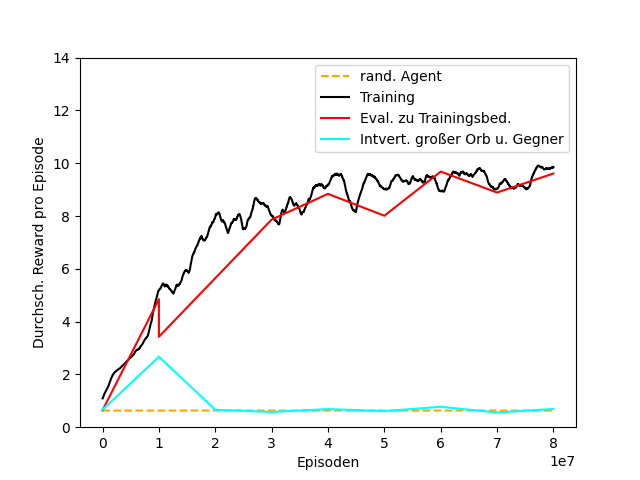
\includegraphics[scale=0.5]{abb/_graphen/semChange_geistGrOrb_80Mio_15act_training_}
        \caption{Evaluation zu Trainingsbed. und mit Invertierung der Geister und gr. Orbs}
        \label{fig:semChange_geistGrOrb_80Mio_15act_training_}
    \end{minipage}
\end{figure}
\begin{center}
 \begin{table}[htp!]
 \begin{center}
  \begin{tabular}{ l c c c }
    \hline
		               			& Zeitschritte & Anzahl Level & 	 Invertierung\\ \hline
     Training              			& 80 Mio       & unbeschr.	    & 	 keine \\ \hline
     Eval. zu Trainingsbed.		& -	        	     & 50		    &	 keine \\ \hline
     Eval. Invertierung		 	& -	        	     & 50		    &	 Geister u. gr. Orbs \\ \hline
    \hline
  \end{tabular}
  \caption{Übersicht über geltende Rahmenbedingungen in Training und Evaluation - 14.}
  \label{tab:tab_durch_EXP_trainSetting13}
  \end{center}
 \end{table}
\end{center} 

\textbf{Diskussion:} Die Evaluation mit der semantischen Invertierung der Geister und den großen Orbs (hier in cyan) entspricht der Intuition, die das vorangegangene Experiment suggeriert. Wie zuvor oszilliert die Performance des Agenten der Checkpoints 20 bis 80 Mio. eng um den Random-Agenten. Lediglich der Checkpoint bei 10 Mio. Zeitschritten weist einen Reward, höher als der des Random-Agenten, in Höhe von $2,67$ auf. Dieser Checkpoint schafft 10\% der Evaluations-Level. Diese semantische Invertierung ist in diesem Environment die mit den geringsten Veränderungen der Pixel-Verteilung und dennoch erreicht der Agent keinen durchschnittlichen Reward $\geq 10$.

\paragraph{Antwort: Set 3, Punkt 2}
Die Antwort dieses Experiments ist ebenso klar zu beantworten, wie die des vergangenen Experiments. Auch wenn der Reward des Agent beim Checkpoint bei 10 Mio. Zeitschritten überhalb dem des Random-Agenten ist, so liegen alle anderen Checkpoints nahe um den Reward des Random-Agenten. Der Agent scheitert somit eindeutig in der Evaluation. Eine mögliche Erklärung für den Ausreißer bei 10 Mio. ist, dass der Object Recognition Layer zu diesem Zeitpunkt im Training noch nicht so stark overfitted, wie bei den folgenden Checkpoints. Aufgrund dessen ist der Agent in der Lage in dieser veränderten Umgebung zu assimilieren und zielführende Entscheidungen zu treffen. 
















\newpage














%....

\section{Ausblick}\label{ausblick}

% - Set 2 Frage 1
% 	- Würde der Agent jemals ein unbekanntes Level schaffen? Er müsste verstehen, dass er sich merken muss, wo er schon war. Würde ein ausreichend langes Training dafür sorgen, dass der Agent die Level konsistent schafft? Dann vielleicht sogar besser, als ein Agent der im Training diese Information zur Verfügung hatte? 

%- Abweichungen vom Pixel-Stream  
%	- Wie wirken sich Änderungen im Pixel-Stream aus? 
%	- Wie ist die Korrelation zwischen Änderungen in der Pixel-Verteilung mit der allgemeinen Performance zusammen?
	
Über die Ausarbeitung der Experimente sind an einigen Stellen Fragen aufgekommen, welche hier aufgegriffen werden. Die Experimente in Unterkapitel \ref{subsec:absch_EXP_durch_reproduktion_generalisierung} zeigen, dass eine Generalisierungslücke entsteht, wenn man auf einer beschränkten Anzahl an Leveln trainiert. Trainiert man einen Agenten für dieselbe Dauer mit einer unbeschränkten Anzahl an Trainings-Leveln, wird diese Lücke geschlossen. Da alle Experimente dieser Arbeit lediglich mit einem Seed für die prozedurale Generierung ausgeführt sind, kann die Aussage, dass die prozedurale Generierung hilft die Lücke zu schließen nur für diesen einen Seed beantwortet werden. Ein ähnliches Experiment über mehrere Seeds hinweg würde diese Aussage bekräftigen und die Hypothese der Autoren von Procgen unterstützen, dass die Procgen-Environments gut geeignet sind, um die Generalisierung und Sample Efficiency eines Algorithmus oder einer Architektur zu evaluieren. 

In den Experimenten zur Beantwortung der Fragen aus Set 2, Punkt 2 (\ref{subsec_EXP_durch_fragen}), ist der Agent von Abbildung \ref{fig:grph_green_80Mio_inflvl_15act_Training_evalAsTraining} in der Lage mit einer ihm unbekannten Orb-Farbe nahezu identische Rewards zu erzielen, wie mit der ihm bekannten Farbe. Diese Ergebnisse werden im darauffolgenden Experiment unter Bedingungen untersucht, die diesen Fakt genauer darstellen sollen. Die Ergebnisse können jedoch nicht reproduziert werden. Das bringt die Frage auf, ob nahezu identischen Rewards mit zwei Orb-Farben lediglich Zufall sind oder ob hier eine unbekannte Korrelation zwischen den beiden Farben besteht, die dem Agenten geholfen hat. Es wäre auch denkbar, dass eine farbunabhängige Korrelation zwischen den Durchläufen besteht, die dem Agenten zu dieser Performance verhilft.

Das Experiment in \ref{par:durch_EXP_farbÄnd_Speichervermögen} untersucht, wie viele Level mit der verwendeten Architektur auswendig gelernt werden können und welche Auswirkungen die visuelle Information der Orbs dabei hat. Hierbei zeigt sich der Trend, dass die Agenten, welche mit visuellen Orb-Information trainiert sind zwar konstant mehr Rewards bekommen, sich jedoch den Rewards der Agenten ohne visuelle Orb-Information mehr und mehr anpassen. Dieses Experiment in größerem Maßstab könnte zeigen, ob sich der Reward des Agenten mit visueller Information der Orbs, asymptotisch an die Rewards der anderen Agenten annähert oder ob die visuelle Orb-Information eine höhere Untergrenze setzt. Das würde die Hypothese aus \ref{sub_absch_EXP_durch_serie1_orbsMaskieren} unterstützen, dass die Orbs eine notwendige bzw. sehr hilfreiche visuelle Information im Chaser-Environment darstellen. 

Die Experimente zur visuellen semantischen Invertierung (\ref{absch_EXP_durch_serie1}) zeigen eindeutig, dass diese Veränderung die Performance der Agenten auf die des Random-Agenten abfallen lässt. Videoanalysen der Evaluation beider Invertierungen zeigen, dass die Agenten zu keinem Zeitpunkt zielführende Entscheidungen treffen können. Daraus kann man schließen, dass die Objekt-Detektion und Objekt-Erkennung der Agenten stark auf die jeweiligen Texturen und Farben der vertauschten Sprites overfitted und die Mechanik der Spielelemente wenig bis keine Auswirkung auf Erkennung und Detektion der Spielelemente hat. Hier ist interessant, ob die Änderung der Pixel-Verteilung von Training zu Evaluation durch mindern der visuellen Komplexität des Agenten-Inputs, semantische Invertierungen in der Evaluation erlauben würde. Eine Möglichkeit die visuelle Komplexität zu mindern wäre alle Texturen in Chaser durch einfarbige, solide Farben zu ersetzten. Die Feature-Extraction-Pipeline hätte somit lediglich farbliche Unterscheidung zwischen den Objekten zur Verfügung. Das könnte der Pipeline erlauben Features aus anderen Information, wie bspw. Bewegungsmuster oder Mechaniken von Spielelementen zu extrahieren.

Des Weiteren kann man hinterfragen, ob der Agent des Experiments zur semantischen Invertierung nur scheitert, da die Änderung in der Evaluation unbekannt ist. Darauf aufbauend kann man untersuchen, ob ein Agent mit ausreichend Zeitschritten im Training jede Änderung des Environments lernen kann. Würde man in Chaser nach jeder Episode dem Orb eine zufällige andere Farbe zuweisen, kann man hiermit erneut untersuchen, ob der Agent die Evaluation mit mehreren Orb-Farben besser besteht als in dieser Arbeit. 


\newpage

\section{Konklusion}\label{konklusion}

%- optische Abweichung von Trainings- zu Evaluation-Umgebung haben fatale Auswirkungen auf die Performance 
%	- Herleitung durch Orbs maskieren 
%		- visuell nicht vorhanden 
%		
%	- Überleitung zu Abstufungen grün 
%	- Hinleitung zu RGB 
%	- !!! Eine Veränderung der Pixel-Verteilung hat starke Auswirkungen auf die allgemeine Performance 

Ziel dieser Arbeit ist die Untersuchung der Generalisierung des eingesetzten IMPALA-Netzwerks \ref{absch_setup_impala} im Zusammenspiel mit dem verwendeten PPO Algorithmus \ref{absch_RL_ppo} in der Procgen-Umgebung \cite{cobbe2019procgen}. Dies geschieht anhand unterschiedlicher visueller Augmentationen des Trainings und/oder der Evaluation. Für die Untersuchung werden drei Sets an Fragen verwendet, welche sich jeweils mit unterschiedlichen Thematiken befassen. 

Das erste Set untersucht die Auswirkung der prozeduralen Level-Generierung auf die Generalisierung des Agenten. Hier wird vorab die verwendete Implementierung auf ihre Richtigkeit überprüft und mit den Ergebnissen des Procgen-Papers (\cite{cobbe2019procgen}) verglichen. Der Vergleich zeigte, dass die Implementierung im Stande ist die Ergebnisse des Papers für das Chaser-Environment zu reproduzieren. Das beantwortet die erste Frage des ersten Sets aus \ref{par_EXP_durch_fragen1} mit "Ja". Die Untersuchung zur Auswirkung der prozeduralen Level-Generierung vergleicht zwei Agenten, wobei einer mit einer beschränkten Anzahl (von 200 Leveln) und der andere mit einer unbeschränkten Anzahl an Leveln, beide für 80 Mio. Zeitschritte, trainiert werden. Der Agent mit einer fixen Anzahl an Trainings-Leveln generalisiert zwar ausreichend, um bei der Evaluation in unbekannten Leveln zu bestehen, jedoch weist die Evaluation eine Generalisierungslücke zwischen Training und Evaluation auf. Der Agent mit unbeschränkt vielen Trainings-Leveln ist in der Lage diese Lücke zu schließen. Die Auswirkungen der prozeduralen Generierung und der daraus resultierende, theoretisch endlose Level-Stream für den Agenten, sind somit eindeutig hilfreich, um in unbekannten Leveln besser abzuschneiden. 

Das zweite Set befasst sich mit Farblichen Änderungen der kleinen Orbs und dem Hintergrund des Spiels. Hierbei wird untersucht, welche Auswirkungen die visuelle Information der kleinen Orbs auf die Performance hat und wie robust die Generalisierung eines Agenten gegenüber Farbänderungen der kleinen Orbs ist. Weiter wird in diesem Set untersucht, wie viele Level die verwendete IMPALA-Architektur (\ref{absch_setup_impala}) auswendig lernen kann und welche Rolle die visuelle Orb-Information dabei spielt. Die Beantwortung der ersten beiden Punkte im zweiten Set zeigen auf, dass die Einstellung, welche die Agenten hervorbrachte und welche am besten generalisiert haben, keine Robustheit gegenüber farblichen Änderungen der kleinen Orbs aufweisen. Des Weiteren wird hier gezeigt, dass die visuelle Information des Orbs eine notwendige Hilfe bietet um in der Evaluation erfolgreich zu bestehen. Die Experimente zum Auswendiglernen der Level zeigen, dass die verwendete Architektur in der Lage ist, in 5 Mio. Zeitschritten 3 Level erfolgreich auswendig zu lernen. Maskiert man jedoch im Training und in der Evaluation die Orbs visuell, so kann lediglich ein Leveln gelernt werden. Das und der konstant niedrigere Reward der Agenten ohne visuelle Orb-Information aus Abbildung \ref{fig:grph_green_80Mio_inflvl_15act_Training_evalAsTraining_1to15}, unterstützt die Hypothese aus \ref{sub_absch_EXP_durch_serie1_orbsMaskieren}, dass die Orbs eine notwendige visuelle Information darstellen, um das Chaser-Environment erfolgreich abzuschließen. \\
Allgemein zeigen die Ergebnisse dieses Sets, dass die eingesetzte Implementierung stark auf Farben overfitted und wenig bis garnicht robust gegenüber farblichen Änderungen ist. Die Ergebnisse der Experimente aus Unterkapitel \ref{sub_absch_EXP_durch_farbÄnderungen} untermauern diese Aussage. 

Das dritte Set untersucht die Auswirkungen visueller semantischer Invertierungen, verschiedener Spielelemente während der Evaluation. Hierfür werden in einem Experiment die Sprites von Mauer und kleinem Orb vertauscht und in einem weiteren die Sprites des großen Orbs und der Geister. Die Invertierung von Mauer und kleinem Orb stellt dabei eine größere Veränderung der Pixel-Verteilung dar, als die Invertierung von großen Orbs und Geistern. Die prozedurale Level-Generierung bringt immer mehr kleine Orbs als Mauern auf das Spielfeld. Eine Invertierung dieser beiden Sprites vertauscht somit auch das Verhältnis, wie oft jedes Spielelemente auf dem Spielfeld vorkommt. Die Invertierung von großen Orbs und Geistern stellt im Gegensatz zu der anderen Invertierung keine Veränderung der Pixel-Verteilung dar, da Geister und große Orbs im Verhältnis 1:1 vorkommen. Von beiden gibt es jeweils drei. Jedoch zeigen die Ergebnisse der Experimente, dass die Einstellung, die die Agenten hervorbringt, welche die beste Generalisierung aufweisen, bei dieser Art der Invertierung versagen. Eine Videoanalyse der Evaluation beider Invertierung zeigt ein interessantes Verhalten. In beiden Experimenten hingen die Agenten die meiste Zeit einer Episode in einem Eck des Labyrinths und sind kaum von der Stelle weggekommen, an der sie in der Episode erscheinen sind. Das erklärt die Rewards ähnlich dem Random-Agent. Bei der Analyse der Evaluation wird jedoch ersichtlich, dass sich der Agent aus dem Experiment zur Invertierung von großen Orbs und Geistern nicht davor scheut einen großen Orb alias einen Geist, welcher sich mit dem Bewegungsmuster der Geister auf ihn zubewegt, entgegen zu gehen. Wohingegen ein Geist alias ein großer Orb, welcher stationär an einer Stelle ist, potentiell gemieden wird. \\
Zusammen mit den Ergebnissen des vorangegangenen Sets kann man davon ausgehen, dass die Feature-Extraction-Pipeline stark auf die Texturen der jeweiligen Spielelemente overfitted und eine Invertierung zweier Sprites, selbst wenn sie im Verhältnis 1:1 vorkommen, eine unüberwindbare Hürde darstellen. \newline

Wie in Kapitel \ref{hauptabschnitt_2} bereits erwähnt, besteht in RL generell das Problem des Overfittings und die daraus resultierende schlechte Generalisierung. Die prozedurale Generierung von Procgen schafft es im Chaser-Environment die Generalisierungslücke zu schließen \ref{subsec:absch_EXP_durch_reproduktion_generalisierung}. Der Agent mit unbeschränkter Level-Anzahl im Training zeigt zu seinen bekannten Trainingsbedingungen, dass nahezu jedes unbekannte Level beim ersten Versuch geschafft wird. Verändert man jedoch die Farbe eine Spielelements bspw. der Orbs, fällt die Performance auf die des Random-Agenten herab. Diese Generalisierung findet somit nahezu ausschließlich innerhalb der ihm bekannten Pixel-Verteilung des Trainings statt. Das stellt eine weitere Problematik in Simulatoren dar. Arbeiten wie \cite{raileanu2020automatic} bieten die Möglichkeit die Pixel-Verteilung im Training, durch verschiedene visuelle Augmentationen mit einer höheren Diversität zu versehen. Somit kann die Problematik der Generalisierung in Procgen von zwei unterschiedlichen Aspekten angegangen werden. Einerseits mit der prozeduralen Generierung, welche theoretisch unendlich viele Versionen des gleichen Levels bereitstellen kann. Andererseits würde mit einem Ansatz wie in \cite{raileanu2020automatic} oder \cite{zhang2018natural} die visuelle Diversität des Environments erhöht werden. Diese beiden Ansätze schaffen Grundlagen für systematische Generalisierung.




%% Beispiel für Bild mit Fußnote
\begin{figure}[htb]
 \centering
 
\includegraphics[width=0.4\textwidth,angle=45]{abb/logo1}
 \caption[Beispiel einer Bildbeschreibung]{Beispiel einer Bildbeschreibung\footnotemark}
\label{fig:beispiel1}
\end{figure}
\footnotetext{Bildquelle: Beispiel einer Bildquelle}

% Beispiel für Bildintegration
\begin{figure}[htb]
 \centering
 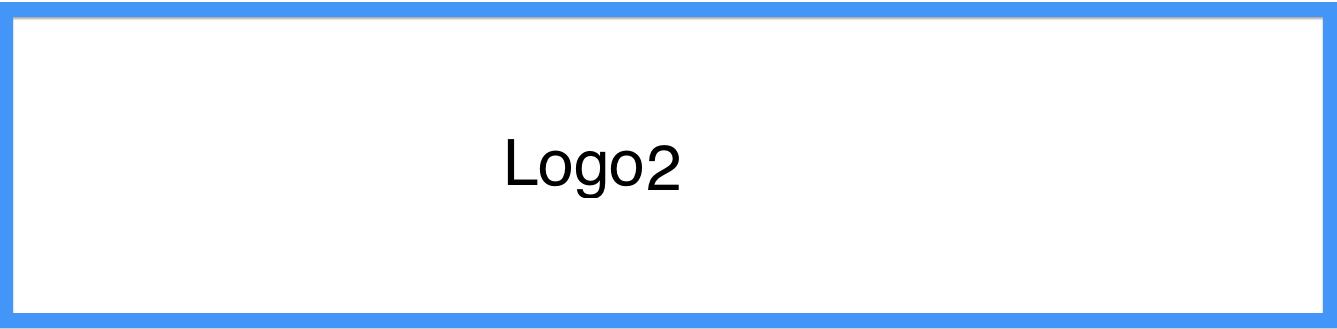
\includegraphics[width=0.3\textwidth,angle=0]{abb/logo2}
 \caption[Beschreibung]{Beschreibung}
\label{fig:Beschreibung}
\end{figure}

% Beispiel: Referenz auf Abbildung
Abbildung~\ref{fig:Beschreibung} [S.\pageref{fig:Beschreibung}]

% Beispiel: Tabelle
\begin{center}
  \begin{tabular}{ | l | c | }
    \hline
    Überschrift 1 & Überschrift 2 \\ \hline \hline
    Info 1 & Info 2 \\ \hline
    Info 3 & Info 4 \\ \hline
    \hline
    \multicolumn{2}{|c|}{Info in einer Zelle} \\
    \hline
  \end{tabular}
\end{center}


% Beispiel für Quellcode Listings
\lstset{language=xml}
\begin{lstlisting}[frame=htrbl, caption={Die Datei {\normalfont \ttfamily  data-config.xml} dient als Beispiel für XML Quellcode}, label={lst:dataconfigxml}]
<dataConfig>
  <dataSource type="JdbcDataSource"
              driver="com.mysql.jdbc.Driver"
              url="jdbc:mysql://localhost/bms_db"
              user="root"
              password=""/>
  <document>
    <entity name="id"
        query="select id, htmlBody, sentDate, sentFrom, subject, textBody
        from mail">
    <field column="id" name="id"/>
    <field column="htmlBody" name="text"/>
    <field column="sentDate" name="sentDate"/>
    <field column="sentFrom" name="sentFrom"/>
    <field column="subject"  name="subject"/>
    <field column="textBody" name="text"/>
    </entity>
  </document>
</dataConfig>
\end{lstlisting}

\lstset{language=java}
\begin{lstlisting}[frame=htrbl, caption={Das Listing zeigt Java Quellcode}, label={lst:result2}]
/* generate TagCloud */
Cloud cloud = new Cloud();
cloud.setMaxWeight(_maxSizeOfText);
cloud.setMinWeight(_minSizeOfText);
cloud.setTagCase(Case.LOWER);

/* evaluate context and find additional stopwords */
String query = getContextQuery(_context);
List<String> contextStoplist = new ArrayList<String>();
contextStoplist = getStopwordsFromDB(query);

/* append context stoplist */
while(contextStoplist != null && !contextStoplist.isEmpty())
  _stoplist.add(contextStoplist.remove(0));

/* add cloud filters */
if (_stoplist != null) {
  DictionaryFilter df = new DictionaryFilter(_stoplist);
  cloud.addInputFilter(df);
}
/* remove empty tags */
NonNullFilter<Tag> nnf = new NonNullFilter<Tag>();
cloud.addInputFilter(nnf);

/* set minimum tag length */
MinLengthFilter mlf = new MinLengthFilter(_minTagLength);
cloud.addInputFilter(mlf);

/* add taglist to tagcloud */
cloud.addText(_taglist);

/* set number of shown tags */
cloud.setMaxTagsToDisplay(_tagsToDisplay);
\end{lstlisting}


% Beispiel für Formeln
Die Zuordnung aller möglichen Werte, welche eine Zufallsvariable annehmen kann nennt man \emph{Verteilungsfunktion} von $X$.

\begin{quotation}
Die Funktion F: $\mathbb{R} \rightarrow$ [0,1] mit $F(t) = P (X \le t)$ heißt Verteilungsfunktion von $X$.\footnote{Mustermann, vgl.~\cite{mm2009}~[S.55]}
\end{quotation}

\begin{quotation}
Für eine stetige Zufallsvariable $X: \Omega \rightarrow \mathbb{R}$ heißt eine integrierbare, nichtnegative reelle Funktion $w: \mathbb{R} \rightarrow \mathbb{R}$ mit $F(x) = P(X \le x) = \int_{-\infty}^{x} w(t)dt$ die \emph{Dichte} oder \emph{Wahrscheinlichkeitsdichte} der Zufallsvariablen $X$.\footnote{Mustermann, vgl.~\cite{mf2005}~[S.56]}
\end{quotation}


% einfacher Zeilenabstand
\singlespacing
% Literaturliste soll im Inhaltsverzeichnis auftauchen
\newpage
\addcontentsline{toc}{section}{Literaturverzeichnis}
% Literaturverzeichnis anzeigen
\renewcommand\refname{Literaturverzeichnis}
\bibliography{Hauptdatei}

%% Index soll Stichwortverzeichnis heissen
% \newpage
% % Stichwortverzeichnis soll im Inhaltsverzeichnis auftauchen
% \addcontentsline{toc}{section}{Stichwortverzeichnis}
% \renewcommand{\indexname}{Stichwortverzeichnis}
% % Stichwortverzeichnis endgültig anzeigen
% \printindex

\onehalfspacing
% evtl. Anhang
\newpage
\addcontentsline{toc}{section}{Anhang}
\fancyhead[L]{Anhang} %Kopfzeile links
\subsection*{Anhang}\label{anhang}
\setcounter{page}{1}
\paragraph{Environment - Agenteninput}\label{anh_env_bilder_chaser} \hfill \break
Folgend werden die Environment-Konfigurationen gezeigt, die über den Verlauf der Experimente verwendet wurden.
\begin{figure}[htb!]
   \captionsetup{width=0.30\linewidth} 

    \begin{minipage}{0.3\linewidth}
        \centering
        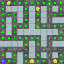
\includegraphics[scale=1.2]{abb/_envpics/example_green}
        \caption*{Default Spiel}
        \label{fig:pic_chaser_defautl}
    \end{minipage}
    %\hfill
    \begin{minipage}{0.3\linewidth}
        \centering
        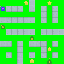
\includegraphics[scale=1.2]{abb/_envpics/example_greenBG}
        \caption*{Hintergrund grün}
        \label{fig:pic_chaser_greenBG}
    \end{minipage}
    \begin{minipage}{0.3\linewidth}
        \centering
        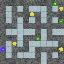
\includegraphics[scale=1.2]{abb/_envpics/example_noVisOrb}
        \caption*{Keine vis. Orbinformation}
        \label{fig:pic_chaser_noVisOrb}
    \end{minipage}
    %\caption{Chaser Environment - links unskaliert, rechts skaliert}
\end{figure}

\begin{figure}[htb!]

   \captionsetup{width=0.30\linewidth} 
    \begin{minipage}{0.3\linewidth}
        \centering
        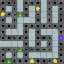
\includegraphics[scale=1.2]{abb/_envpics/example_black}
        \caption*{Schwarze Orbs}
        \label{fig:pic_chaser_blackOrb}
    \end{minipage}
    %\hfill
    \begin{minipage}{0.3\linewidth}
        \centering
        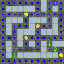
\includegraphics[scale=1.2]{abb/_envpics/example_blue}
        \caption*{Blaue Orbs}
        \label{fig:pic_chaser_blueOrb}
    \end{minipage}
    \begin{minipage}{0.3\linewidth}
        \centering
        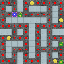
\includegraphics[scale=1.2]{abb/_envpics/example_red}
        \caption*{Rote Orbs}
        \label{fig:pic_chaser_redOrb}
    \end{minipage}
    %\caption{Chaser Environment - links unskaliert, rechts skaliert}
\end{figure}

\begin{figure}[htb!]
    \begin{minipage}{0.3\linewidth}
   \captionsetup{width=0.90\linewidth} 
        \centering
        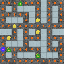
\includegraphics[scale=1.2]{abb/_envpics/example_orbSprite}
        \caption*{Default Spiel mit Orb-Sprite (Flammen)}
        \label{fig:pic_chaser_defaultOrbsprite}
    \end{minipage}
    \begin{minipage}{0.3\linewidth}
   \captionsetup{width=0.90\linewidth} 
        \centering
        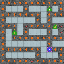
\includegraphics[scale=1.2]{abb/_envpics/example_changedSem_gelbOrb_Enemy}
        \caption*{Sprite-Tausch: großer Orb u. Geist}
        \label{fig:pic_chaser_semChange_yelOrb_enemy}
    \end{minipage}
    \begin{minipage}{0.3\linewidth}
   \captionsetup{width=0.90\linewidth} 
        \centering
        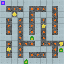
\includegraphics[scale=1.2]{abb/_envpics/example_changedSem_orb_wall}
        \caption*{Sprite-Tausch: kleiner Orb u. Wand}
        \label{fig:pic_chaser_semChange_Orb_wall}
    \end{minipage}
    %\caption{Chaser Environment - links unskaliert, rechts skaliert}
\end{figure}

\begin{figure}[htb!]
    \begin{minipage}{0.3\linewidth}
        \centering
        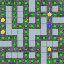
\includegraphics[scale=1.2]{abb/_envpics/example_green_250}
        \caption*{Orb-Farbe: grün:250}
        \label{fig:pic_chaser_green_250}
    \end{minipage}
    \begin{minipage}{0.3\linewidth}
        \centering
        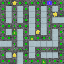
\includegraphics[scale=1.2]{abb/_envpics/example_green_200}
        \caption*{Orb-Farbe: grün:200}
        \label{fig:pic_chaser_green_200}
    \end{minipage}
    %\hfill
    \begin{minipage}{0.3\linewidth}
        \centering
        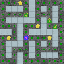
\includegraphics[scale=1.2]{abb/_envpics/example_green_150}
        \caption*{Orb-Farbe: grün:150}
        \label{fig:pic_chaser_green_150}
    \end{minipage}
    %\caption{Chaser Environment - links unskaliert, rechts skaliert}
\end{figure}

\newpage

\begin{figure}[htb!]
    \begin{minipage}{0.3\linewidth}
        \centering
        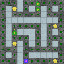
\includegraphics[scale=1.2]{abb/_envpics/example_green_100}
        \caption*{Orb-Farbe: grün:100}
        \label{fig:pic_chaser_green_100}
    \end{minipage}
    \begin{minipage}{0.3\linewidth}
        \centering
        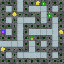
\includegraphics[scale=1.2]{abb/_envpics/example_green_50}
        \caption*{Orb-Farbe: grün:50}
        \label{fig:pic_chaser_green_50}
    \end{minipage}
    %\hfill
    \begin{minipage}{0.3\linewidth}
        \centering
        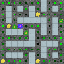
\includegraphics[scale=1.2]{abb/_envpics/example_green_rand}
        \caption*{Orb-Farbe: gruen, zufaellig 0-255}
        \label{fig:pic_chaser_green_random}
    \end{minipage}
    %\caption{Chaser Environment - links unskaliert, rechts skaliert}
\end{figure}

\begin{figure}[htb!]
   \captionsetup{width=0.3\linewidth} 
    \begin{minipage}{0.3\linewidth}
        \centering
        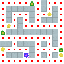
\includegraphics[scale=1.2]{abb/_envpics/example_whiteBG_red}
        \caption*{BG: weiß; \\ Orb: r:255, g:0, b:0}
        \label{fig:pic_chaser_whiteBG_red}
    \end{minipage}
    \begin{minipage}{0.3\linewidth}
        \centering
        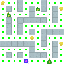
\includegraphics[scale=1.2]{abb/_envpics/example_whiteBG_green}
        \caption*{BG: weiß; \\ Orb: r:0, g:255, b:0}
        \label{fig:pic_chaser_whiteBG_green}
    \end{minipage}
    %\hfill
    \begin{minipage}{0.3\linewidth}
        \centering
        \includegraphics[scale=1.2]{abb/_envpics/example_whiteBG_blue}
        \caption*{BG: weiß; \\ Orb: r:0, g:0, b:255}
        \label{fig:pic_chaser_whiteBG_blue}
    \end{minipage}
    %\caption{Chaser Environment - links unskaliert, rechts skaliert}
\end{figure}


\paragraph{Beispiel Topologie eines dreischichtigen MLP}
\label{anh_mlp_L3}
Folgend ist ein Beispiel für den topologischen Aufbau eines Feed Forward MLP gegeben. 

\begin{figure}[htb!]
    \begin{minipage}{\linewidth}
        \centering
        \includegraphics[scale=0.4]{abb/maucher_bsp_MLP}
        \caption*{Darstellung eines MLP mit drei Schichten \cite{maucher_ki_09}}
        \label{fig:pic_L3_mlp}
    \end{minipage}
\end{figure}
\newpage


\paragraph{Hyperparameter} \label{hyperparameter}
Folgend sind die verwendeten Hyperparameter in tabellarischer Form aufgearbeitet. 

\begin{center}
 \begin{table}[htb!]
 \begin{center}
  \begin{tabular}{c | c}
     Hyperparameter 		& Setting   \\ \hline \hline
     Learning Rate 		& 0,00025 \\ \hline 
     Entropie Koeffizient 	& 0,01 \\ \hline 
     Value Funciton Koeff.	& 0,5 \\ \hline 
     gamma $(\gamma)$	& 0,999 \\ \hline 
     lambda $(\lambda)$	& 0,95 \\ \hline 
     Anzahl Zeitschritte $T$	& 256  \\ \hline 
     Anzahl Minibatches	& 8  \\ \hline 
     Anzahl Epochen		& 3  \\ \hline 
     Clipping Range		& 0,2  \\ \hline 
  \end{tabular}
  \caption{Übersicht über die verwendeten Hyperparameter für PPO.}
  \label{tab:tab_durch_EXP_trainSetting3}
  \end{center}
 \end{table}
\end{center} 

\paragraph{Hardware} \label{hardware}
Folgend ist die verwendete Hardware in tabellarischer Form aufgelistet. Die Experimente werden auf dem Servern der Hochschule der Medien ausgeführt. Genauer wurde der GLaDOS-Server des Institute for Applied Artificial Intelligence verwendet. 

\begin{center}
 \begin{table}[htb!]
 \begin{center}
  \begin{tabular}{c | c}
    \hline
     	 				& GLaDOS   \\ \hline 
     Host 				& glados.mi.hdm-stuttgart.de        \\ \hline 
     CPU 				& i7-6950X (10-core) @ 3.0GHz \\ \hline 
     GPU				& 4x NVIDIA TITAN Xp 12GB        \\ \hline 
     Memory			& 128GB (8x 16GB) DDR4 PC2400 \\ \hline 
     
    \hline
  \end{tabular}
  \caption{Übersicht über die verwendete Hardware.}
  \label{tab:tab_durch_EXP_trainSetting3}
  \end{center}
 \end{table}
\end{center} 
\null\newpage

\paragraph{IMPALA-Architektur}\label{anh_impala_arch} \hfill \break
Folgend ist die IMPALA-Architektur aus dem Paper \cite{espeholt2018impala} dargestellt. Der Output dieser Architektur liefert den Input für sowohl die Policy-Approximation, als auch die Value-Function-Approximation.
\begin{figure}[htb!]
    \begin{minipage}{\linewidth}
        \centering
        \includegraphics[angle=90,origin=c,scale=0.3]{abb/_networkArch/impala_net_arch}
        \caption*{Vereinfacht dargestellte IMPALA-Architektur}
        \label{fig:pic_impala_net_arch}
    \end{minipage}
\end{figure}
\vfill


\begin{figure}[htb!]
    \hspace*{-1.5cm}
    \begin{minipage}{\linewidth}
        \centering
        \includegraphics[scale=0.25]{abb/_networkArch/conv_seq_1}
        \caption*{Erste Convolutional Sequenz}
        \label{fig:pic_impala_net_arch}
    \end{minipage}
\end{figure}
\begin{figure}[htb!]
    \hspace*{-1.5cm}
    \begin{minipage}{\linewidth}
        \centering
        \includegraphics[scale=0.25]{abb/_networkArch/conv_seq_2}
        \caption*{Zweite Convolutional Sequenz}
        \label{fig:pic_impala_net_arch}
    \end{minipage}
\end{figure}
\begin{figure}[htb!]
    \hspace*{-1.5cm}
    \begin{minipage}{\linewidth}
        \centering
        \includegraphics[scale=0.25]{abb/_networkArch/conv_seq_3}
        \caption*{Dritte Convolutional Sequenz}
        \label{fig:pic_impala_net_arch}
    \end{minipage}
\end{figure}

\paragraph{Experiment - 5 Mio. Zeitschritte, Grüner und Normaler Hintergrund}\label{anh_exp_5mio} \hfill \break
Folgend sind zwei Experimente mit zwei unterschiedlichen Agenten beschrieben. Hier werden beide Agenten für 5 Mio. Zeitschritte in einem einzigen Level trainiert. Das Training der beiden Agenten unterscheidet sich lediglich im verwendeten Hintergrund. Die genauen Trainingsbedingungen können Tabelle \ref{tab:tab_durch_EXP_trainSetting_anh_1} entnommen werden.

Abbildung \ref{fig:grph_green_80Mio_200lvl_15act_Training_evalAsTraining_5Mio1} zeigt das Training mit normalem Hintergrund. Abbildung \ref{fig:grph_green_80Mio_inflvl_15act_Training_evalAsTraining_5Mio2} zeigt das Training mit dem grünen Hintergrund.

\begin{figure}[htp!]
   \centering
   \captionsetup{width=0.45\linewidth} 
    \begin{minipage}{0.48\linewidth}
        \centering\
        \textbf{Normaler Hintergrund\\0 bis 15 Level}\par\medskip
        \includegraphics[scale=0.5]{abb/_graphen/tTimesteps_eprewmean_smooth_normal}
        \caption{Training mit normalem Hintergrund für 5 Mio. Zeitschritte.}
        \label{fig:grph_green_80Mio_200lvl_15act_Training_evalAsTraining_5Mio1} 
    \end{minipage}
    \centering
    \begin{minipage}{0.48\linewidth}
        \centering
        \textbf{Grüner Hintergrund\\0 bis 15 Level}\par\medskip
        \includegraphics[scale=0.5]{abb/_graphen/tTimesteps_eprewmean_smooth_green} 
        \caption{Training mit grünem Hintergrund für 5 Mio. Zeitschritte.}
        \label{fig:grph_green_80Mio_inflvl_15act_Training_evalAsTraining_5Mio2}
    \end{minipage}
\end{figure}

\begin{center}
%\vskip-0.5cm
 \begin{table}[htb!]
 \begin{center}
  \begin{tabular}{ l c c c c }
    \hline
			       				& Zeitschritte 	& Anzahl Level 	& Hintergrund	 	& Farbe Orb \\ \hline \hline
     Training normaler Hintergrund  	& 5 Mio       	& 1		&  normal			& r:0, g:255, b:0 \\ \hline
     Training grüner Hintergrund   	& 5 Mio       	& 1 		&  r:0, g:255, g:0	& r:0, g:255, b:0 \\ \hline
    \hline
  \end{tabular}
  \caption{Übersicht über geltende Rahmenbedingungen in Training und Evaluation - 15.}
  \label{tab:tab_durch_EXP_trainSetting_anh_1}
  \end{center}
 \end{table}
\end{center} 
\vfill

\paragraph{Erfolgsrate Experiment zum Speichervermögen}\label{anh_exp_erfolgsrate}
Die folgende Tabelle zeigt die Erfolgsrate des jeweils letzten Checkpoints aller Agenten des Experiments \ref{par:durch_EXP_farbÄnd_Speichervermögen}.

\begin{center}
%\vskip-0.5cm
 \begin{table}[htb!]
 \begin{center}
  \begin{tabular}{ l c c  }
    \hline
	       				& Erfolgsrate \%, norm. BG 	& Erfolgsrate \%, grüner BG \\ \hline \hline
     Checkpoint 1  		&  98      			& 78		 \\ \hline
     Checkpoint 2  		& 90       			& 20		 \\ \hline
     Checkpoint 3  		& 76       			& 8		 \\ \hline
     Checkpoint 4  		& 56       			& 4		 \\ \hline
     Checkpoint 5  		& 54       			& 0		 \\ \hline
     Checkpoint 6 	 	& 64       			& 0		 \\ \hline
     Checkpoint 7  		& 52       			& 2		 \\ \hline
     Checkpoint 8	  	& 24       			& 0		 \\ \hline
     Checkpoint 9  		& 4       			& 4		 \\ \hline
     Checkpoint 10  		& 4       			& 4		 \\ \hline
     Checkpoint 11		& 34       			& 0		 \\ \hline
     Checkpoint 12		& 8       			& 0		 \\ \hline
     Checkpoint 13		& 4       			& 0		 \\ \hline
     Checkpoint 14  		& 10       			& 2		 \\ \hline
     Checkpoint 15  		& 8       			& 0		 \\ \hline
    \hline
  \end{tabular}
  \caption{Übersicht über die Erfolgsrate der Agenten mit normalem und grünem Hintergrund.}
  \label{tab:tab_durch_EXP_trainSetting5}
  \end{center}
 \end{table}
\end{center} 

\paragraph{Konzept des Convolutional Filtering}\label{anh_convConcept}
Die folgende Abbildung zeigt einen Schritt des Convolutional Filtering anhand eines zweidimensionalen Inputs. 
Diese Abbildung dient einer bildlichen Veranschaulichung des in Abschnitt \ref{absch_RL_convNets} vorgestellten Konzepts von Convolutional-Layers.

\begin{figure}[htb!]
 \centering
 \includegraphics[scale=0.36]{abb/maucher_ConvolutionConcept}
 \caption[Beschreibung]{Darstellung des Konzepts des Convolutional Filtering \cite{maucher_nb_cnn}. }
\label{fig:maucher_cnn}
\end{figure}

\paragraph{Convolutional-Layer für 2D-Input}\label{anh_conv2d}
Die folgende Abbildung zeigt eine Berechnung eines Features aus einem zweidimensionalen Convolutional-Layer. Weiter zeigt das Bild die jeweiligen geteilten Gewichte (hier in rot und blau). Die Kernel Size ist hier $[3 \times 3]$. Somit teilen sich die Neuronen $x_{11}, x_{12}, ..., x_{33}$ eine Gewichtsmatrix. Dasselbe gilt für jeden Block des Inputs der Größe $[3 \times 3]$, wie in Abbildung \ref{fig:maucher_cnn2d} ersichtlich. 

\begin{figure}[htb!]
 \centering
 \includegraphics[scale=0.4]{abb/maucher_2dConvLayer}
 \caption[Beschreibung]{Darstellung einer Single Feature Map, extrahiert aus einem einkanäligen, zweidimensionalen Convolutional-Layer \cite{maucher_nb_cnn}. }
\label{fig:maucher_cnn2d}
\end{figure}



\pagebreak
% Eidesstattliche Erklärung
\pagestyle{empty}
\newpage
\addcontentsline{toc}{section}{Eidesstattliche Erklärung}
\null\newpage
\section*{Eidesstattliche Erklärung}
\thispagestyle{empty}
\begin{verbatim}

\end{verbatim}

\begin{center}
\begin{LARGE}Eidesstattliche Erklärung zur Arbeit\end{LARGE} 
\newline
\newline
\begin{LARGE}Deep Reinforcement Learning\end{LARGE}
\newline
\begin{verbatim}

\end{verbatim} 

Wie wirkt sich die visuelle Augmentation des Environments auf die Generalisierung eines RL-Agenten in Procgen aus?
\end{center}
\begin{verbatim}


\end{verbatim}
Ich versichere, die von mir vorgelegte Arbeit selbstständig verfasst zu haben. Alle Stellen, die wörtlich oder sinngemäß aus veröffentlichten oder nicht veröffentlichten Arbeiten anderer entnommen sind, habe ich als entnommen kenntlich gemacht. Sämtliche Quellen und Hilfsmittel, die ich für die Arbeit benutzt habe, sind angegeben. Die Arbeit hat mit gleichem Inhalt bzw. in wesentlichen Teilen noch keine anderen Prüfungsbehörde vorgelegt bekommen.



\begin{displaymath}
% use packages: array
\begin{array}{ll}
Unterschrift:~~~~~~~~~~~~~~~~~~~~~~~~~~~~~~~~~~~~~~~~~~
& Ort, Datum:~~~~~~~~~~~~~~~~~~~~~~~~~~~~~~~~~~~~~~~~~~
\end{array}
\end{displaymath}


% leere Abschlussseite
\newpage
\thispagestyle{empty} % erzeugt Seite ohne Kopf- / Fusszeile
\mbox{}

\end{document}
